\documentclass[11pt, a4paper]{article}

\usepackage{amsfonts}
\usepackage{amssymb}
\usepackage{amsmath}
\usepackage{epsfig}
\usepackage{graphicx}
\usepackage{tabularx}
\usepackage{parskip}
\usepackage[margin=2.54cm]{geometry}
\usepackage[colorlinks=true]{hyperref}
\usepackage[sort]{natbib}

%%%%%%%%%%%%%%%%%%%%%%%%%%%%%%%%%%%%%%%%%%%%%%%%%%%%%%%%%%%%%%%%%%%%%%%%%%%%%%%%%
%%%%%%%%%%%%%%%%%%%%%%%%%%%%%%%%%%%%%%%%%%%%%%%%%%%%%%%%%%%%%%%%%%%%%%%%%%%%%%%%%
\title{Tag growth}

\author{D'Arcy N. Webber, Jim Thorson}

\date{\today}

\begin{document}
\maketitle

%%%%%%%%%%%%%%%%%%%%%%%%%%%%%%%%%%%%%%%%%%%%%%%%%%%%%%%%%%%%%%%%%%%%%%%%%%%%%%%%%
%%%%%%%%%%%%%%%%%%%%%%%%%%%%%%%%%%%%%%%%%%%%%%%%%%%%%%%%%%%%%%%%%%%%%%%%%%%%%%%%%
%%%%%%%%%%%%%%%%%%%%%%%%%%%%%%%%%%%%%%%%%%%%%%%%%%%%%%%%%%%%%%%%%%%%%%%%%%%%%%%%%
\section{Introduction}
%%%%%%%%%%%%%%%%%%%%%%%%%%%%%%%%%%%%%%%%%%%%%%%%%%%%%%%%%%%%%%%%%%%%%%%%%%%%%%%%%
%%%%%%%%%%%%%%%%%%%%%%%%%%%%%%%%%%%%%%%%%%%%%%%%%%%%%%%%%%%%%%%%%%%%%%%%%%%%%%%%%
%%%%%%%%%%%%%%%%%%%%%%%%%%%%%%%%%%%%%%%%%%%%%%%%%%%%%%%%%%%%%%%%%%%%%%%%%%%%%%%%%
\textit{Dissostichus mawsoni}

Key words: Antarctic toothfish, Ross Sea


Variation among individuals can be included by treating each individual's
demographic parameters as a random effect that arises from a population-level
distribution. We start with the specialised von Bertalanffy growth function
\begin{equation}
  \frac{dL}{dt} = a - k L,
\end{equation}
where $\frac{dL}{dt}$ is change in length as a function of time $t$, $a$ scales
with energy acquisition, and $k$ represents metabolic upkeep costs. However,
individuals that are more highly active may obtain more food (increased $a$)
and simultaneously have greater upkeep costs (increased
$k$). Following~\citealp{Shelton2013}, we include the correlation via the
following equation
\begin{equation}
  a = \gamma k^\psi,
\end{equation}
where $\gamma$ and $\psi$ approximate the allometric scaling of energy costs
and aquisition. Integration then yeilds
\begin{equation}
  L(t + \Delta_t) = L(t) e^{-k_i \Delta_t} + k_i^{\psi - 1} \left( 1 - e^{-k_i}
  \right) \gamma \sum_{j=0}^{\Delta_t - 1} e^{-k_i j}.
\end{equation}
When $\psi = 0$ this model become the classic von Bertallanffy.

\begin{align}
  \frac{dL}{dt} &= \gamma k^\psi - k L,\\
  &= \gamma - k L \quad \text{if} \quad \psi = 0,
\end{align}

\begin{align}
  L_\infty &= \frac{\gamma k^\psi}{k},\\
  &= \frac{\gamma}{k} \quad \text{if} \quad \psi = 0, 
\end{align}

\begin{align}
  \gamma &= \frac{k L_\infty}{k^\psi},\\
  &= k L_\infty \quad \text{if} \quad \psi = 0, 
\end{align}


\begin{equation}
  L_0 = L_\infty \left( 1 - e^{k t_0} \right),
\end{equation}
$L_0$ is the length at time 0.

\begin{align}
  c_v &= \frac{\sigma}{\mu},\\
  \sigma &= c_v \mu,\\
  \varepsilon &\sim \mathcal{N} \left( 0, \sigma^2_o L_t \right),
\end{align}


\begin{table}[!htbp]
  \begin{quote}
    \caption{\label{tab:Dunn} The values of the standard von Bertalanffy growth
      function etsimated bu Dunn et al....} \small{
      \begin{center}
        \begin{tabular}{|ll|rr|}
          \hline
          Parameter & Units          & Female & Male\\
          \hline \hline
          $t_0$     & y              & 0.021 & -0.256\\
          $k$       & $\text{y}^{-1}$ & 0.090 & 0.093\\
          $L_\infty$ & cm              & 180.20 & 169.07\\
          $c_v$     & -               & 0.102 & 0.012\\
          \hline
        \end{tabular}
      \end{center}
    }
  \end{quote}
\end{table}

\begin{equation}
  L_t = L_\infty \left( 1 - e^{-k (t - t_0)} \right),
\end{equation}


%%%%%%%%%%%%%%%%%%%%%%%%%%%%%%%%%%%%%%%%%%%%%%%%%%%%%%%%%%%%%%%%%%%%%%%%%%%%%%%%%
%%%%%%%%%%%%%%%%%%%%%%%%%%%%%%%%%%%%%%%%%%%%%%%%%%%%%%%%%%%%%%%%%%%%%%%%%%%%%%%%%
%%%%%%%%%%%%%%%%%%%%%%%%%%%%%%%%%%%%%%%%%%%%%%%%%%%%%%%%%%%%%%%%%%%%%%%%%%%%%%%%%
\newpage\clearpage
\section{Simulation}
%%%%%%%%%%%%%%%%%%%%%%%%%%%%%%%%%%%%%%%%%%%%%%%%%%%%%%%%%%%%%%%%%%%%%%%%%%%%%%%%%
%%%%%%%%%%%%%%%%%%%%%%%%%%%%%%%%%%%%%%%%%%%%%%%%%%%%%%%%%%%%%%%%%%%%%%%%%%%%%%%%%
%%%%%%%%%%%%%%%%%%%%%%%%%%%%%%%%%%%%%%%%%%%%%%%%%%%%%%%%%%%%%%%%%%%%%%%%%%%%%%%%%
A total of 400 different data sets were simulated, 100 relicates for each of
four different parameter sets. In all data sets 315 individuals were simulated,
the same number as in the actual toothfish data set. The sex, Age1, Age2 and
time at liberty were simulated by
\begin{itemize}
\item Sampling sex from the observed sexes of individuals (with replacement).
\item Sampling Age1, Age2 and time at liberty independently (with replacement)
  from those observed. Randomly selected one of these variables and calculated
  this values given the other two.
\item Rounding Age1, Age2 and time at liberty off to the nearest integer.
\end{itemize}
Initial simulations experiments suggested that the parameter $\psi$ could not
be estimated reliably so this parameter was fixed at zero. The four different
parameter sets used are given in Table~\ref{tab:sims}. The simulated values
used are based on plausible parameter values or values calculated from
Table~\ref{tab:Dunn} above. Notice I had to tone down the $\sigma_o$ to keep
the individual growth trajectories looking resonable. More plots to come.
\begin{table}[!htbp]
  \begin{quote}
    \caption{\label{tab:sims} .} \small{
      \begin{center}
        \begin{tabular}{|l||rr|rr|rr|rr|}
          \hline
          Simulation     & \multicolumn{2}{c|}{v0} & \multicolumn{2}{c|}{v1} &
          \multicolumn{2}{c|}{v2} & \multicolumn{2}{c|}{v3}\\
          \hline
          Parameter      & Female  & Male    & Female & Male & Female & Male & Female & Male\\
          \hline \hline
          $L_0$          & -0.341  & 3.978   & -0.341  & 3.978   & -0.341  & 3.978 & -0.341 & 3.978\\
          $\overline{k}$ & 0.00173 & 0.00179 & 0.00173 & 0.00179 & 0.00173 & 0.00179 & 0.00173 & 0.00179\\
          $\gamma$       & 0.312   & 0.302   & 0.312   & 0.302   & 0.312   & 0.302 & 0.312 & 0.302\\
          \hline
          $\sigma_o$     & 0.102   & 0.102   & 0.050    & 0.050  & 0.050   & 0.050 & 0.050 & 0.050\\
          $\sigma_k$     & -       & -       & 0.1000   & 0.200  & -       & - & 0.100 & 0.200\\
          $\sigma_z$     & -       & -       & -        & -      & 0.200   & 0.400 & 0.20 & 0.40\\
          \hline
        \end{tabular}
      \end{center}
    }
  \end{quote}
\end{table}



%%%%%%%%%%%%%%%%%%%%%%%%%%%%%%%%%%%%%%%%%%%%%%%%%%%%%%%%%%%%%%%%%%%%%%%%%%%%%%%%%
%%%%%%%%%%%%%%%%%%%%%%%%%%%%%%%%%%%%%%%%%%%%%%%%%%%%%%%%%%%%%%%%%%%%%%%%%%%%%%%%%
\newpage\clearpage
\subsection{Fits to simulated data}
%%%%%%%%%%%%%%%%%%%%%%%%%%%%%%%%%%%%%%%%%%%%%%%%%%%%%%%%%%%%%%%%%%%%%%%%%%%%%%%%%
%%%%%%%%%%%%%%%%%%%%%%%%%%%%%%%%%%%%%%%%%%%%%%%%%%%%%%%%%%%%%%%%%%%%%%%%%%%%%%%%%

%%%%%%%%%%%%%%%%%%%%%%%%%%%%%%%%%%%%%%%%%%%%%%%%%%%%%%%%%%%%%%%%%%%%%%%%%%%%%%%%%
\subsubsection{v0}
%%%%%%%%%%%%%%%%%%%%%%%%%%%%%%%%%%%%%%%%%%%%%%%%%%%%%%%%%%%%%%%%%%%%%%%%%%%%%%%%%
No random effects. 97/100 pdH.

\begin{figure}[!htbp]
  \centering
  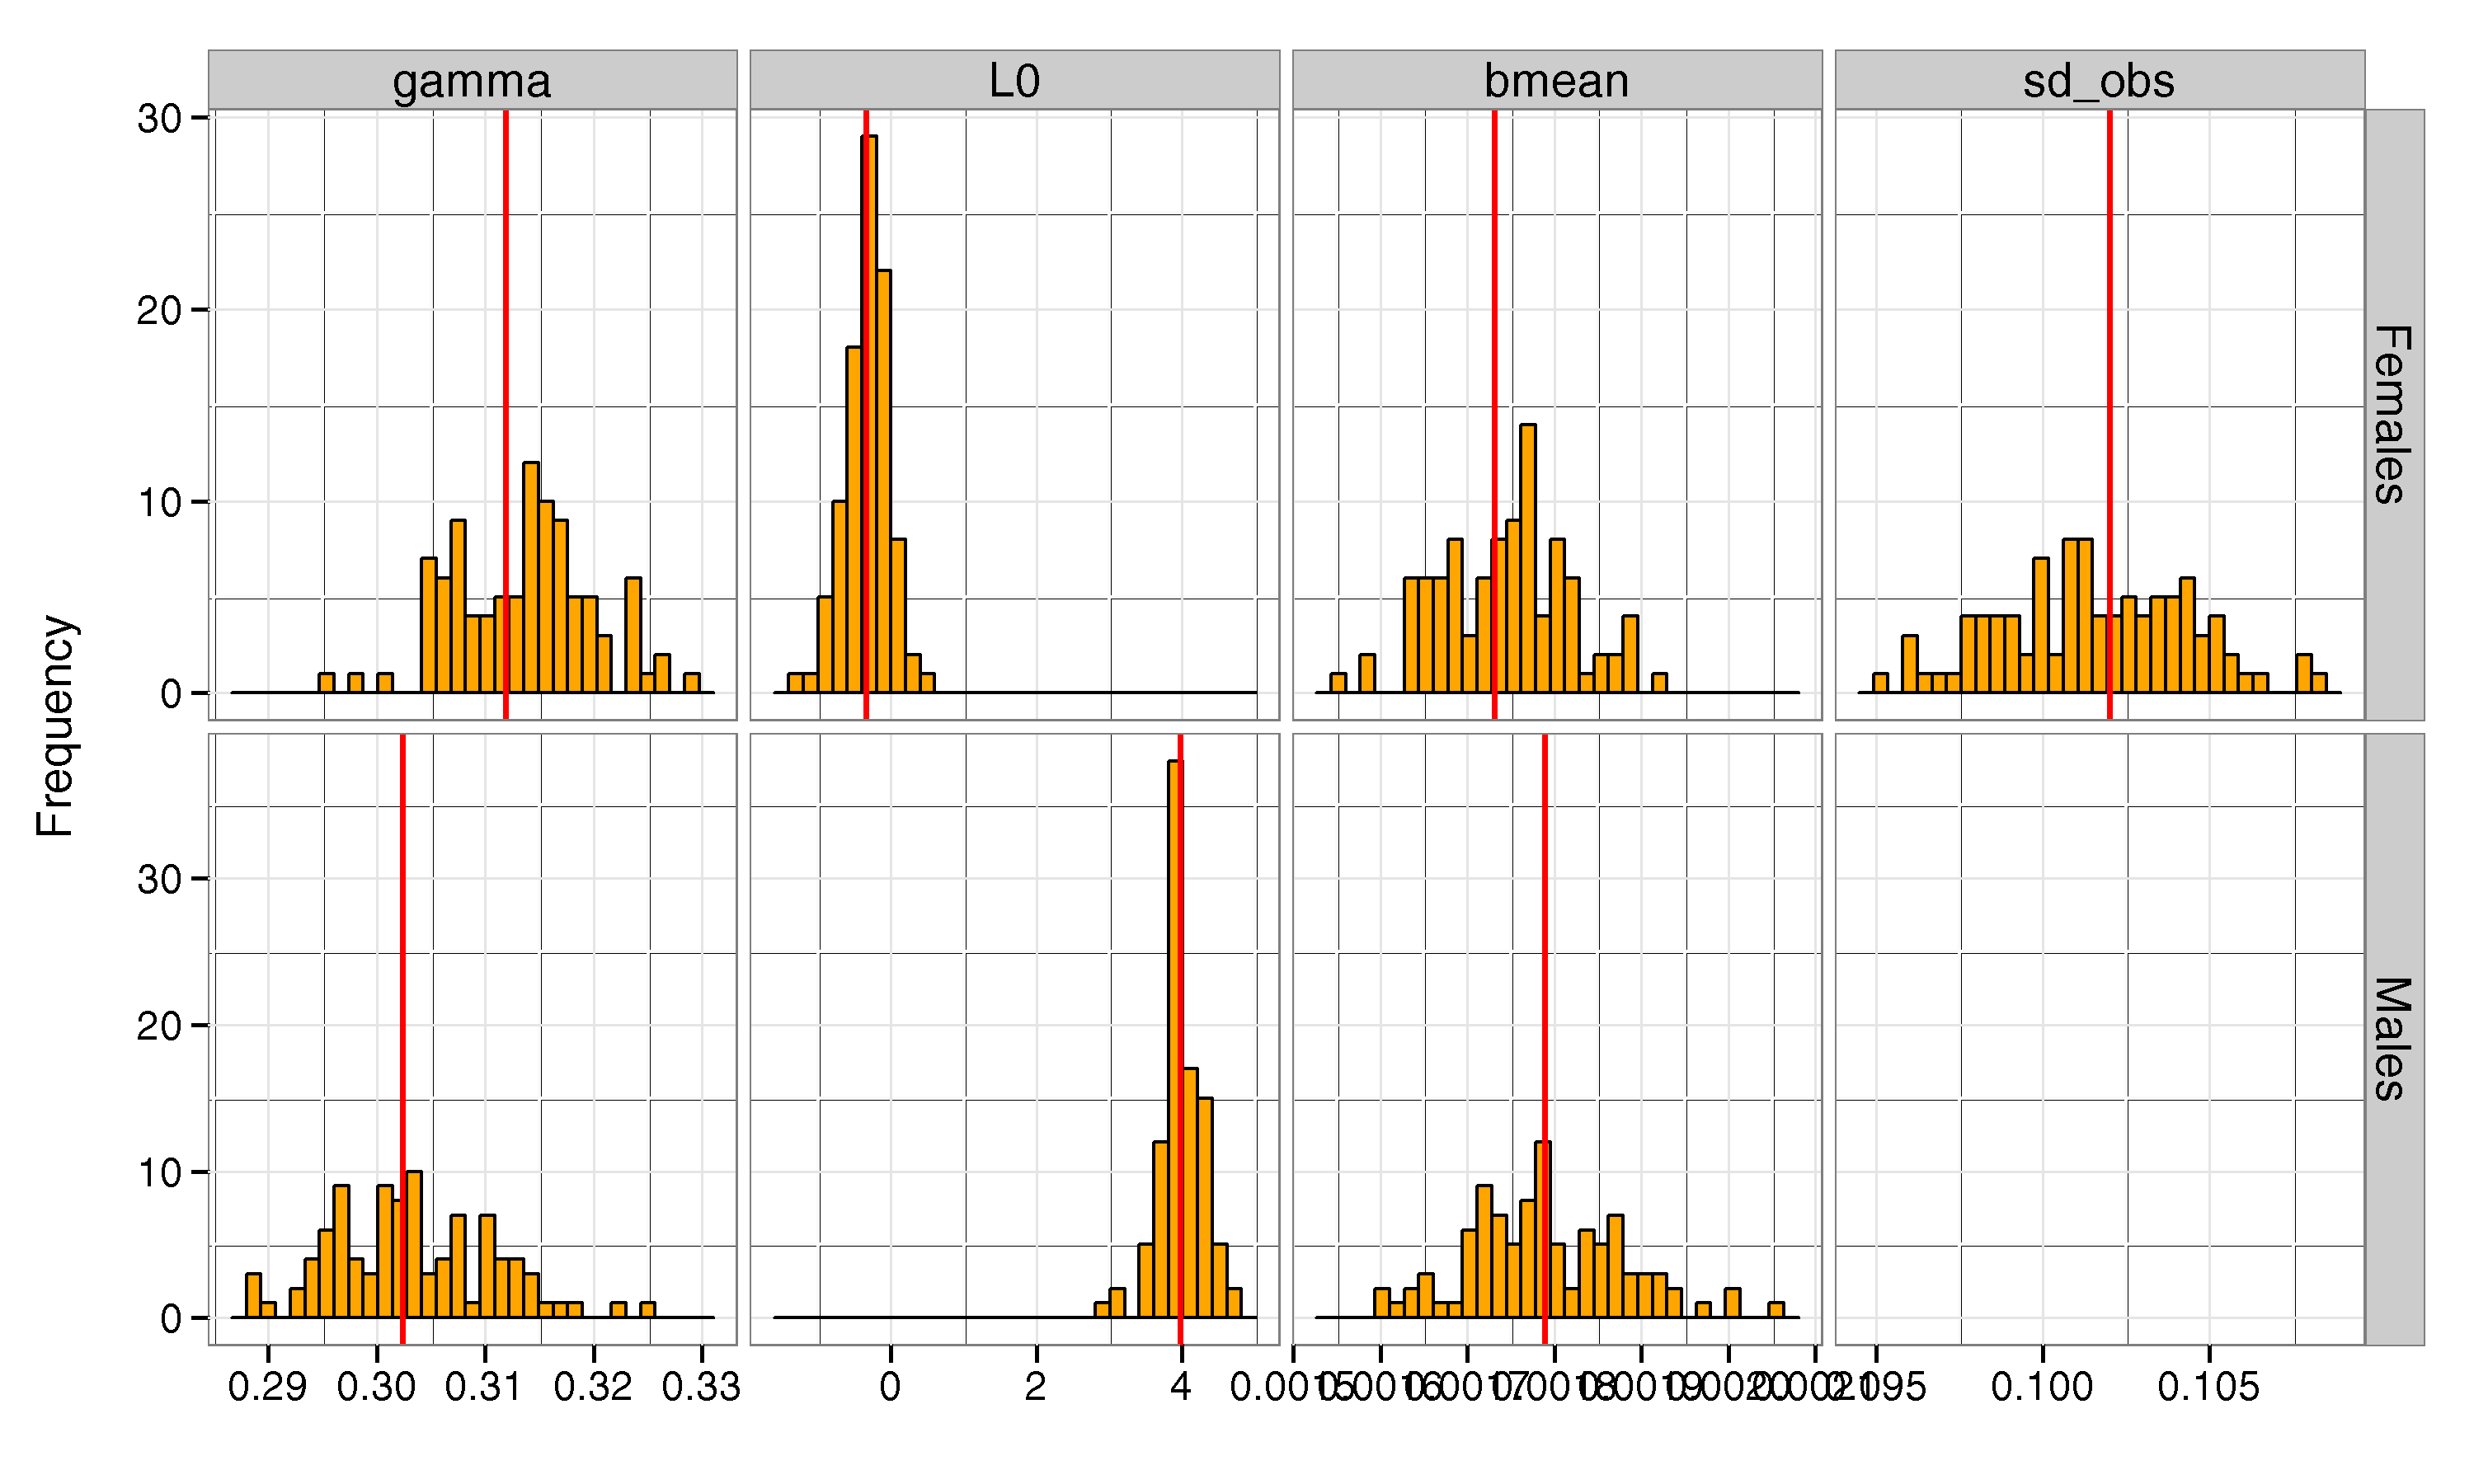
\includegraphics[width=\linewidth]{../simulation/v0/results/SimPars.png}
  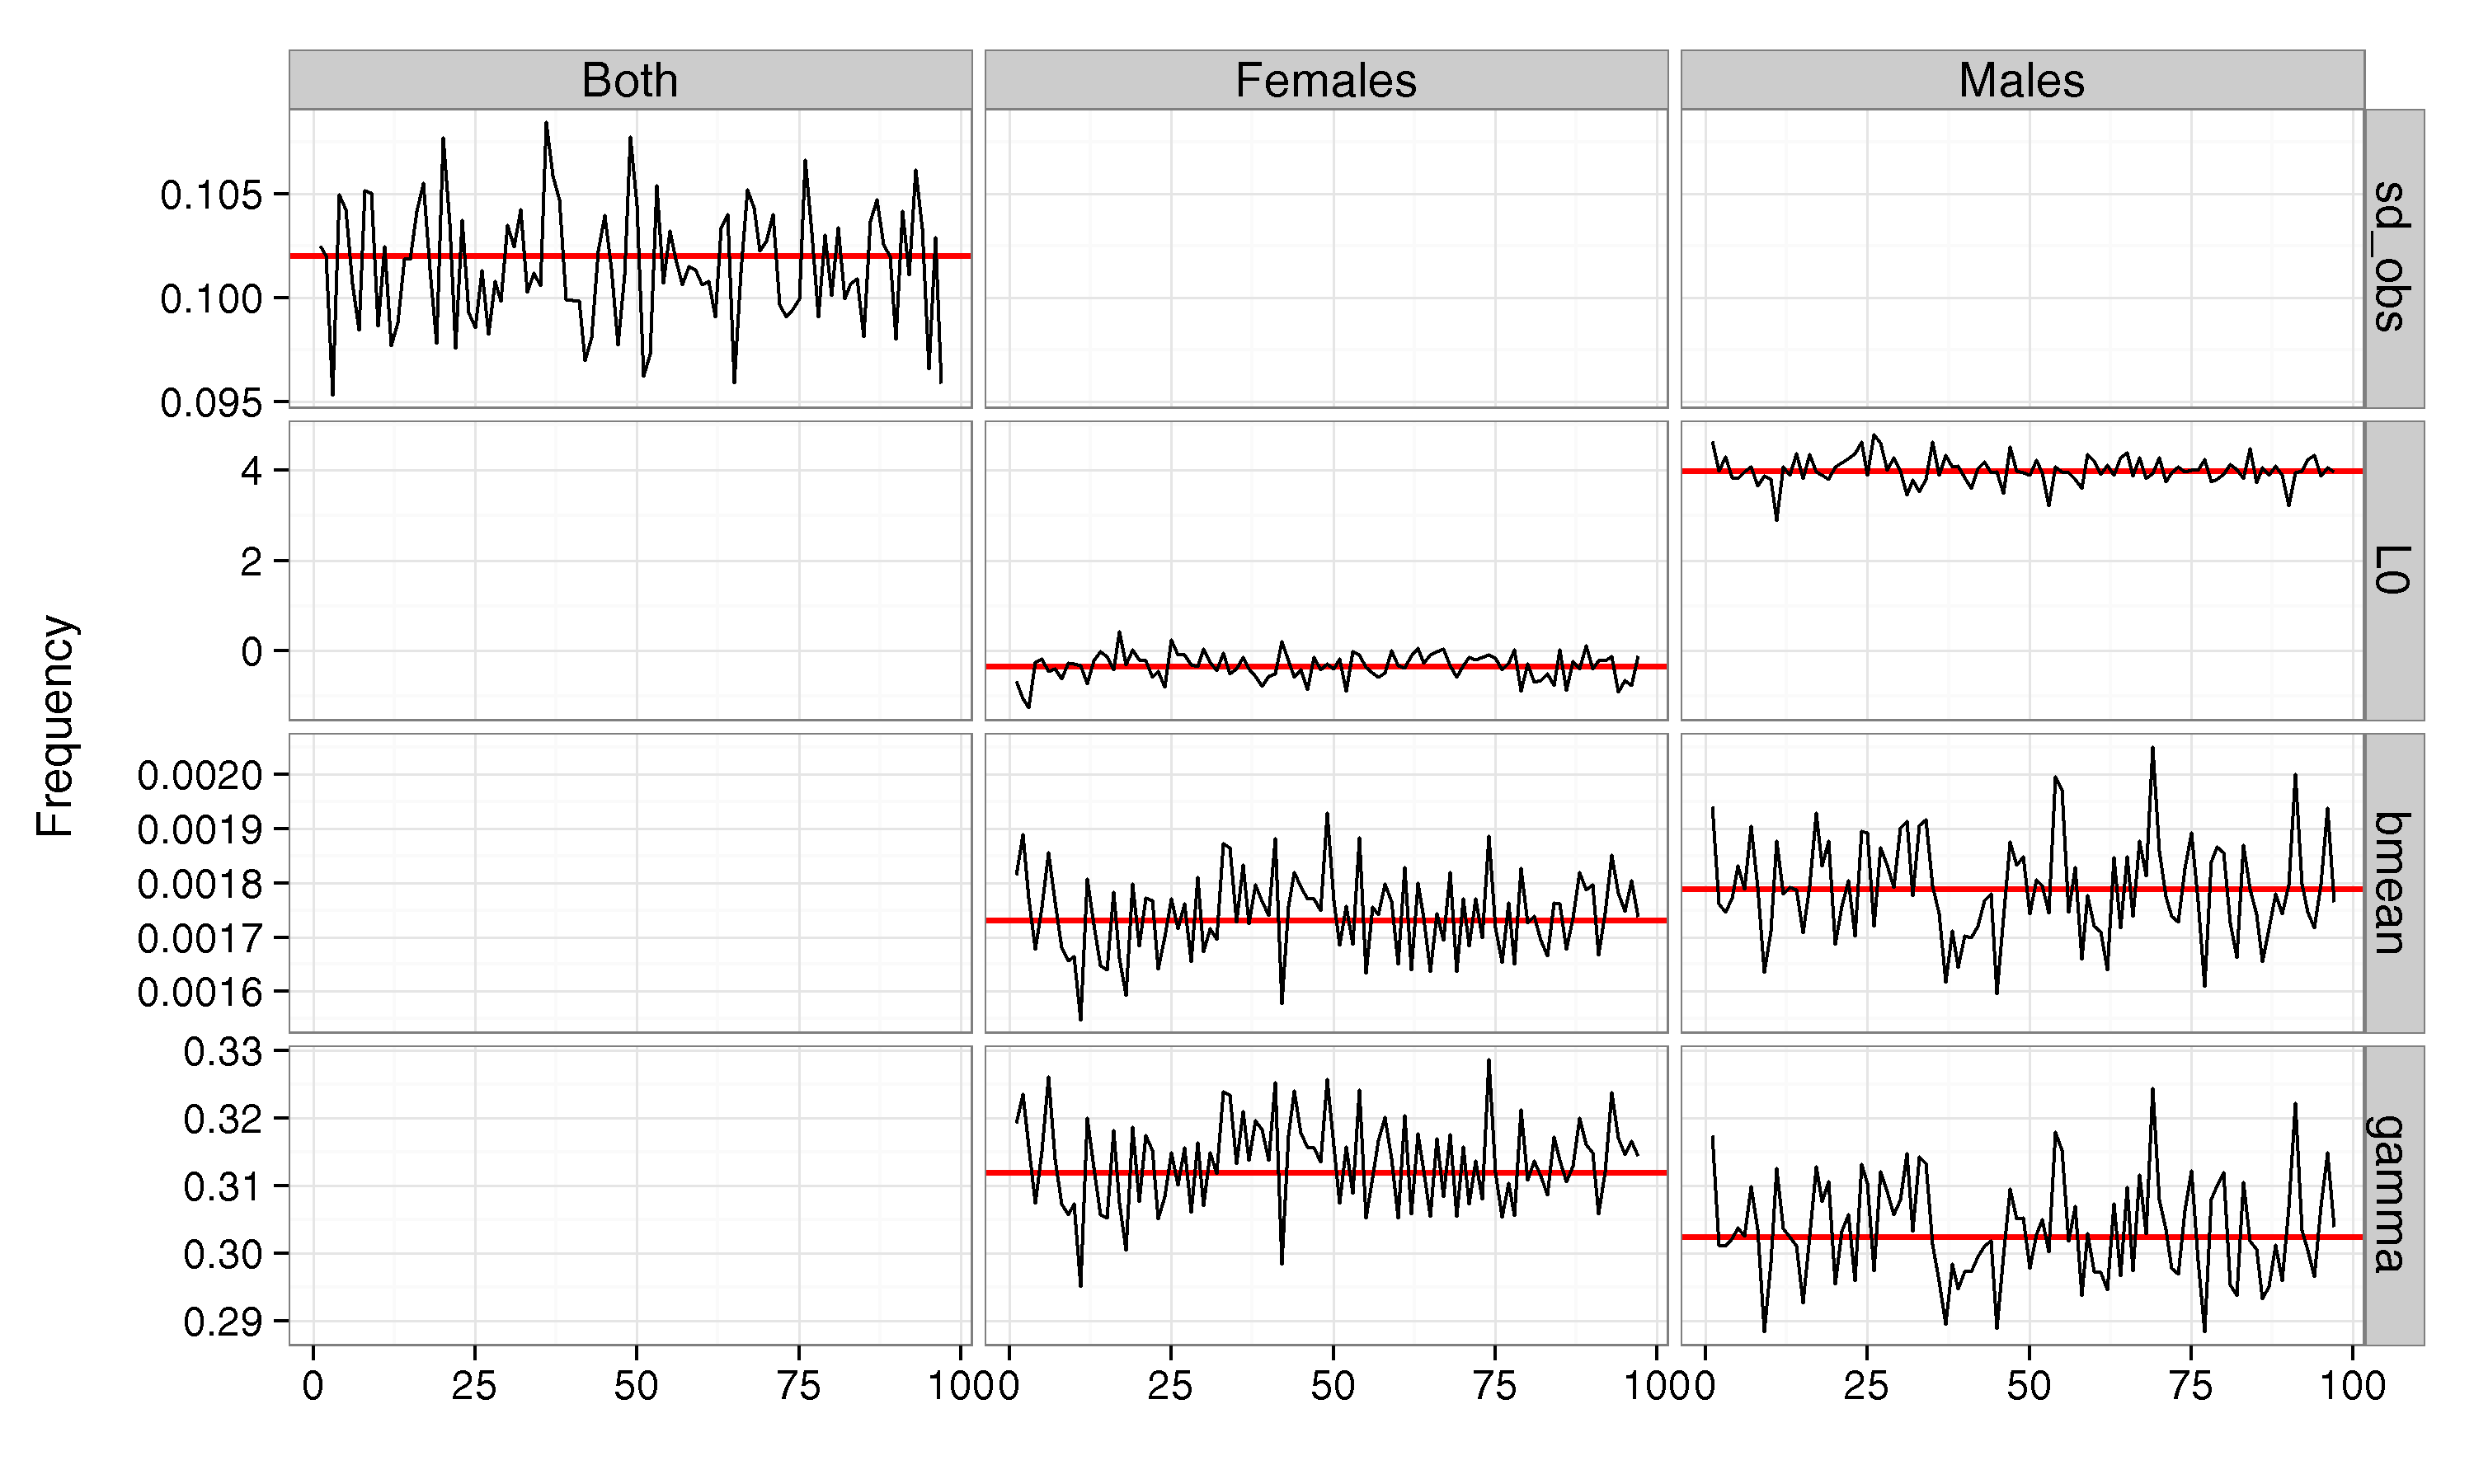
\includegraphics[width=\linewidth]{../simulation/v0/results/TracePars.png}
  \begin{quote}
    \caption{pdH fits plotted only.}
    \label{fig:sims1}
  \end{quote}
\end{figure}

%%%%%%%%%%%%%%%%%%%%%%%%%%%%%%%%%%%%%%%%%%%%%%%%%%%%%%%%%%%%%%%%%%%%%%%%%%%%%%%%%
\newpage\clearpage
\subsubsection{v1}
%%%%%%%%%%%%%%%%%%%%%%%%%%%%%%%%%%%%%%%%%%%%%%%%%%%%%%%%%%%%%%%%%%%%%%%%%%%%%%%%%
Random effects $k$, 78/100 pdH.

\begin{figure}[!htbp]
  \centering
  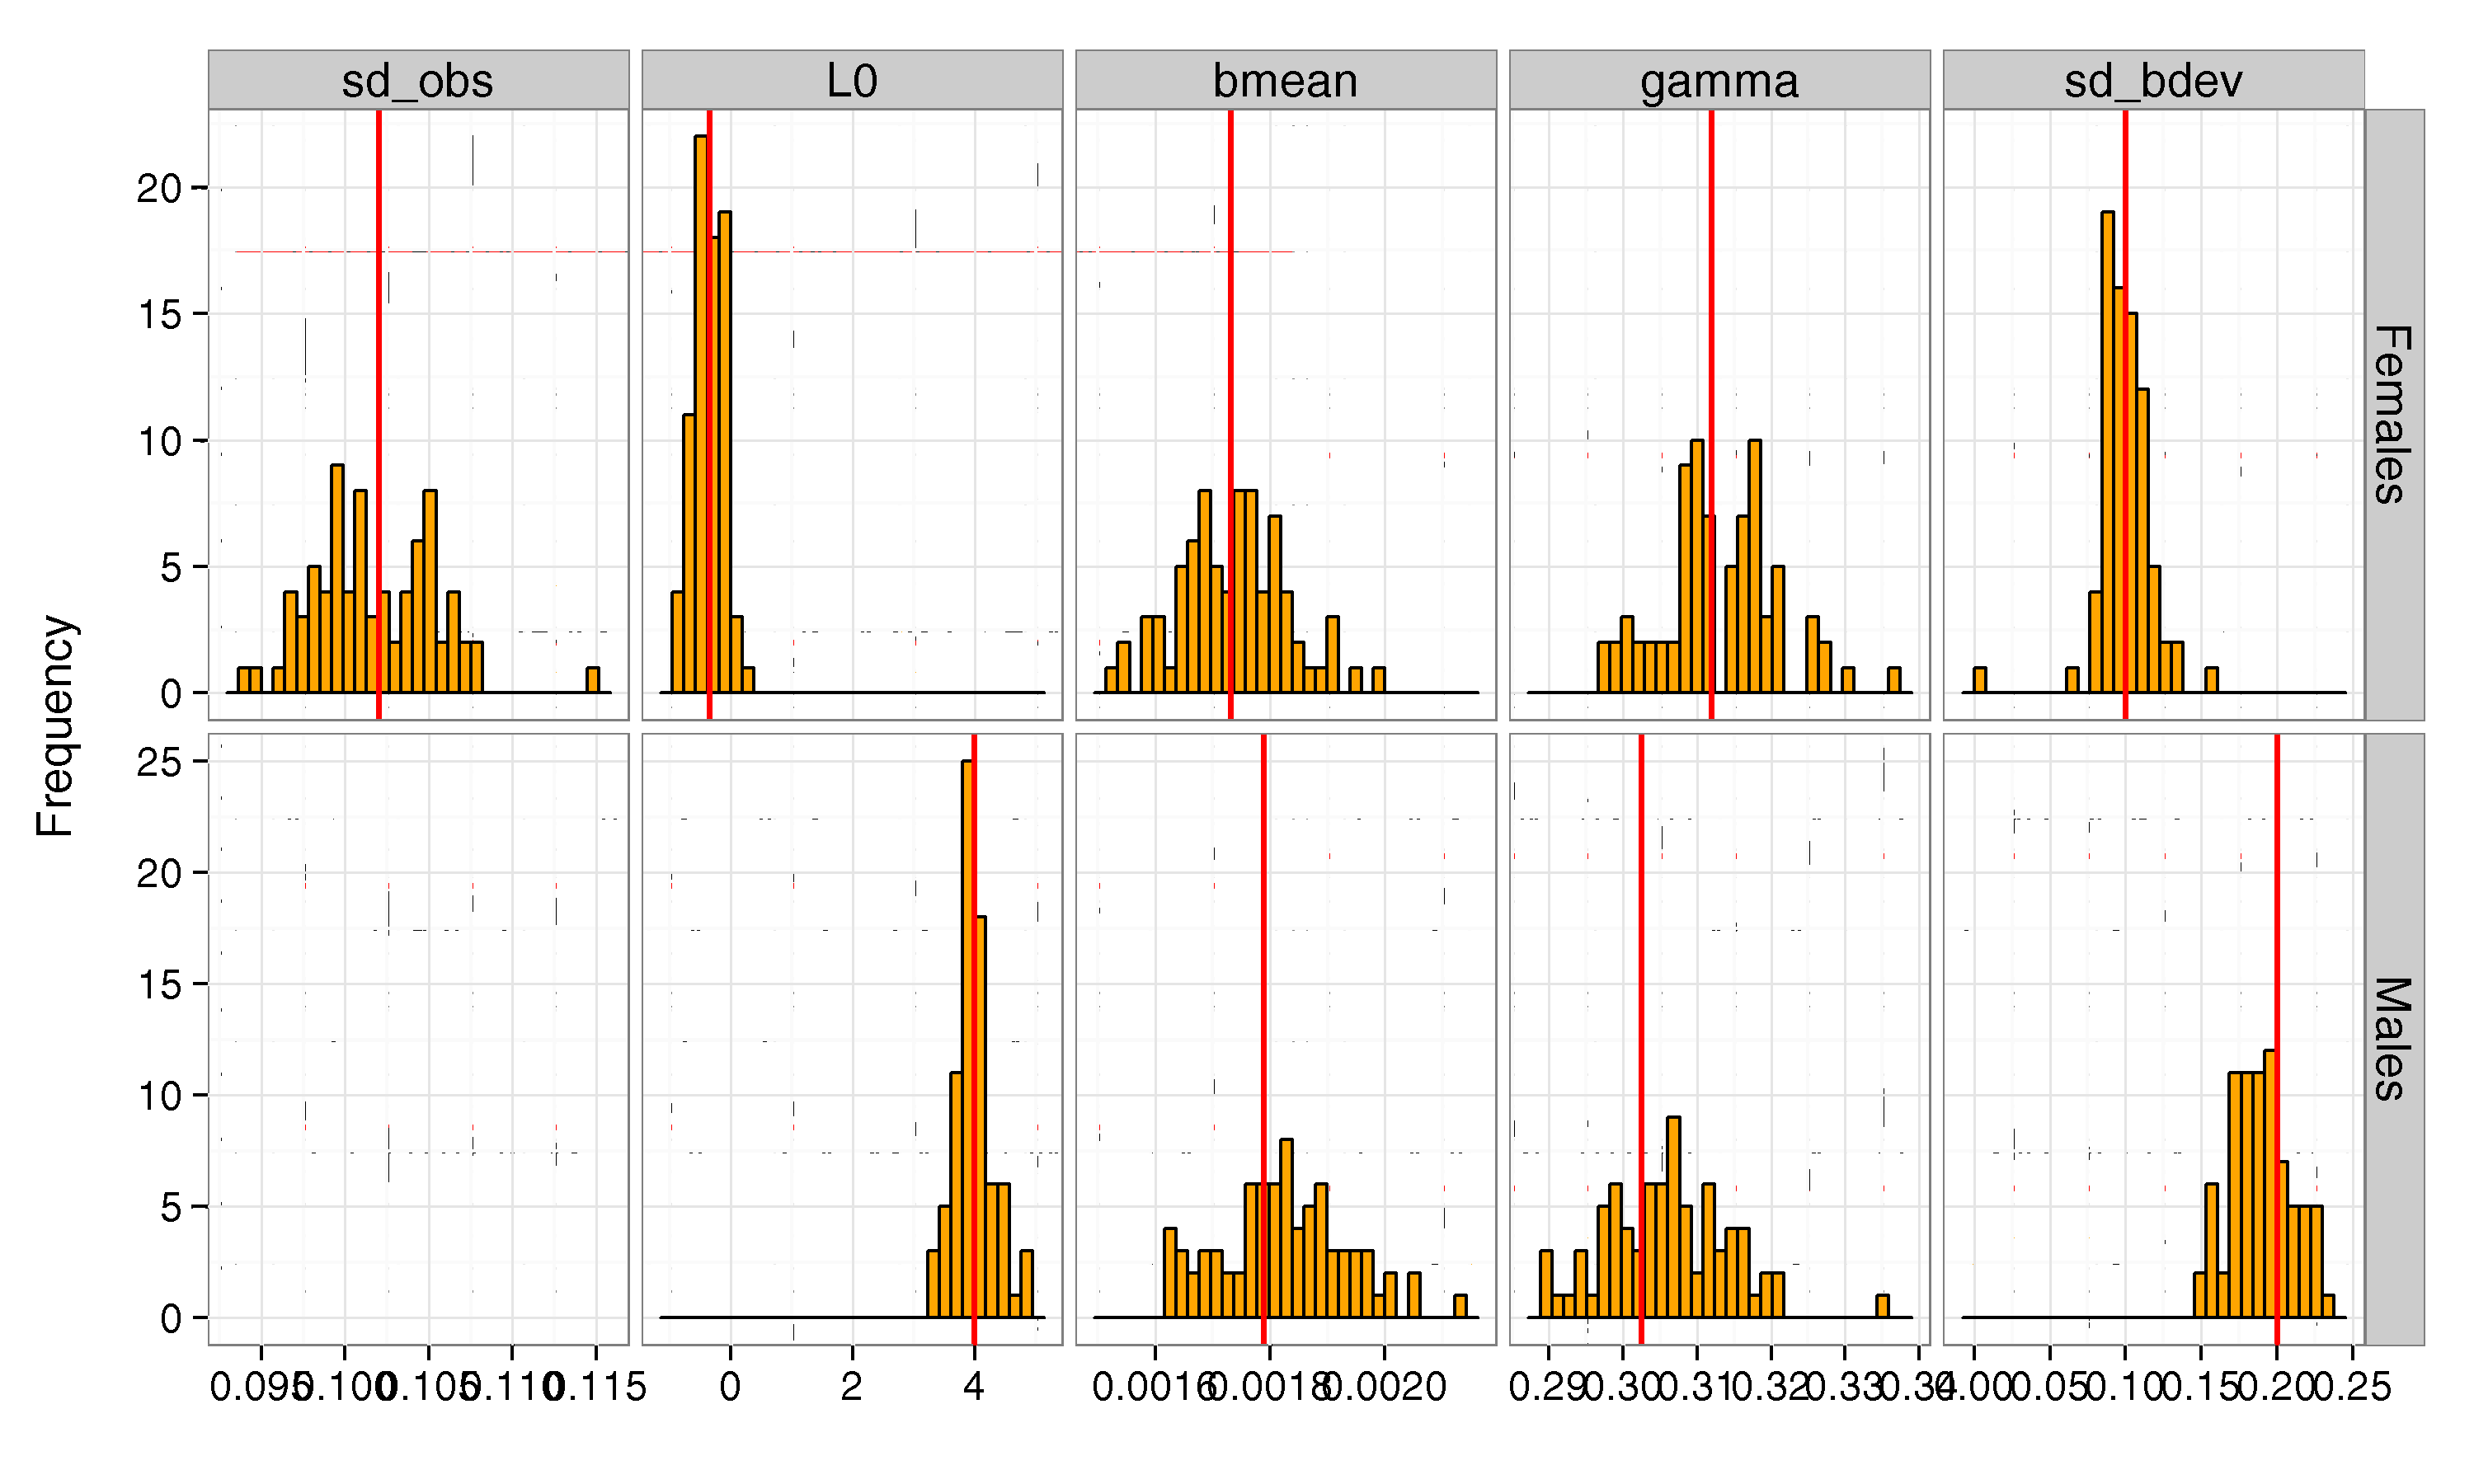
\includegraphics[width=\linewidth]{../simulation/v1/results/SimPars.png}
  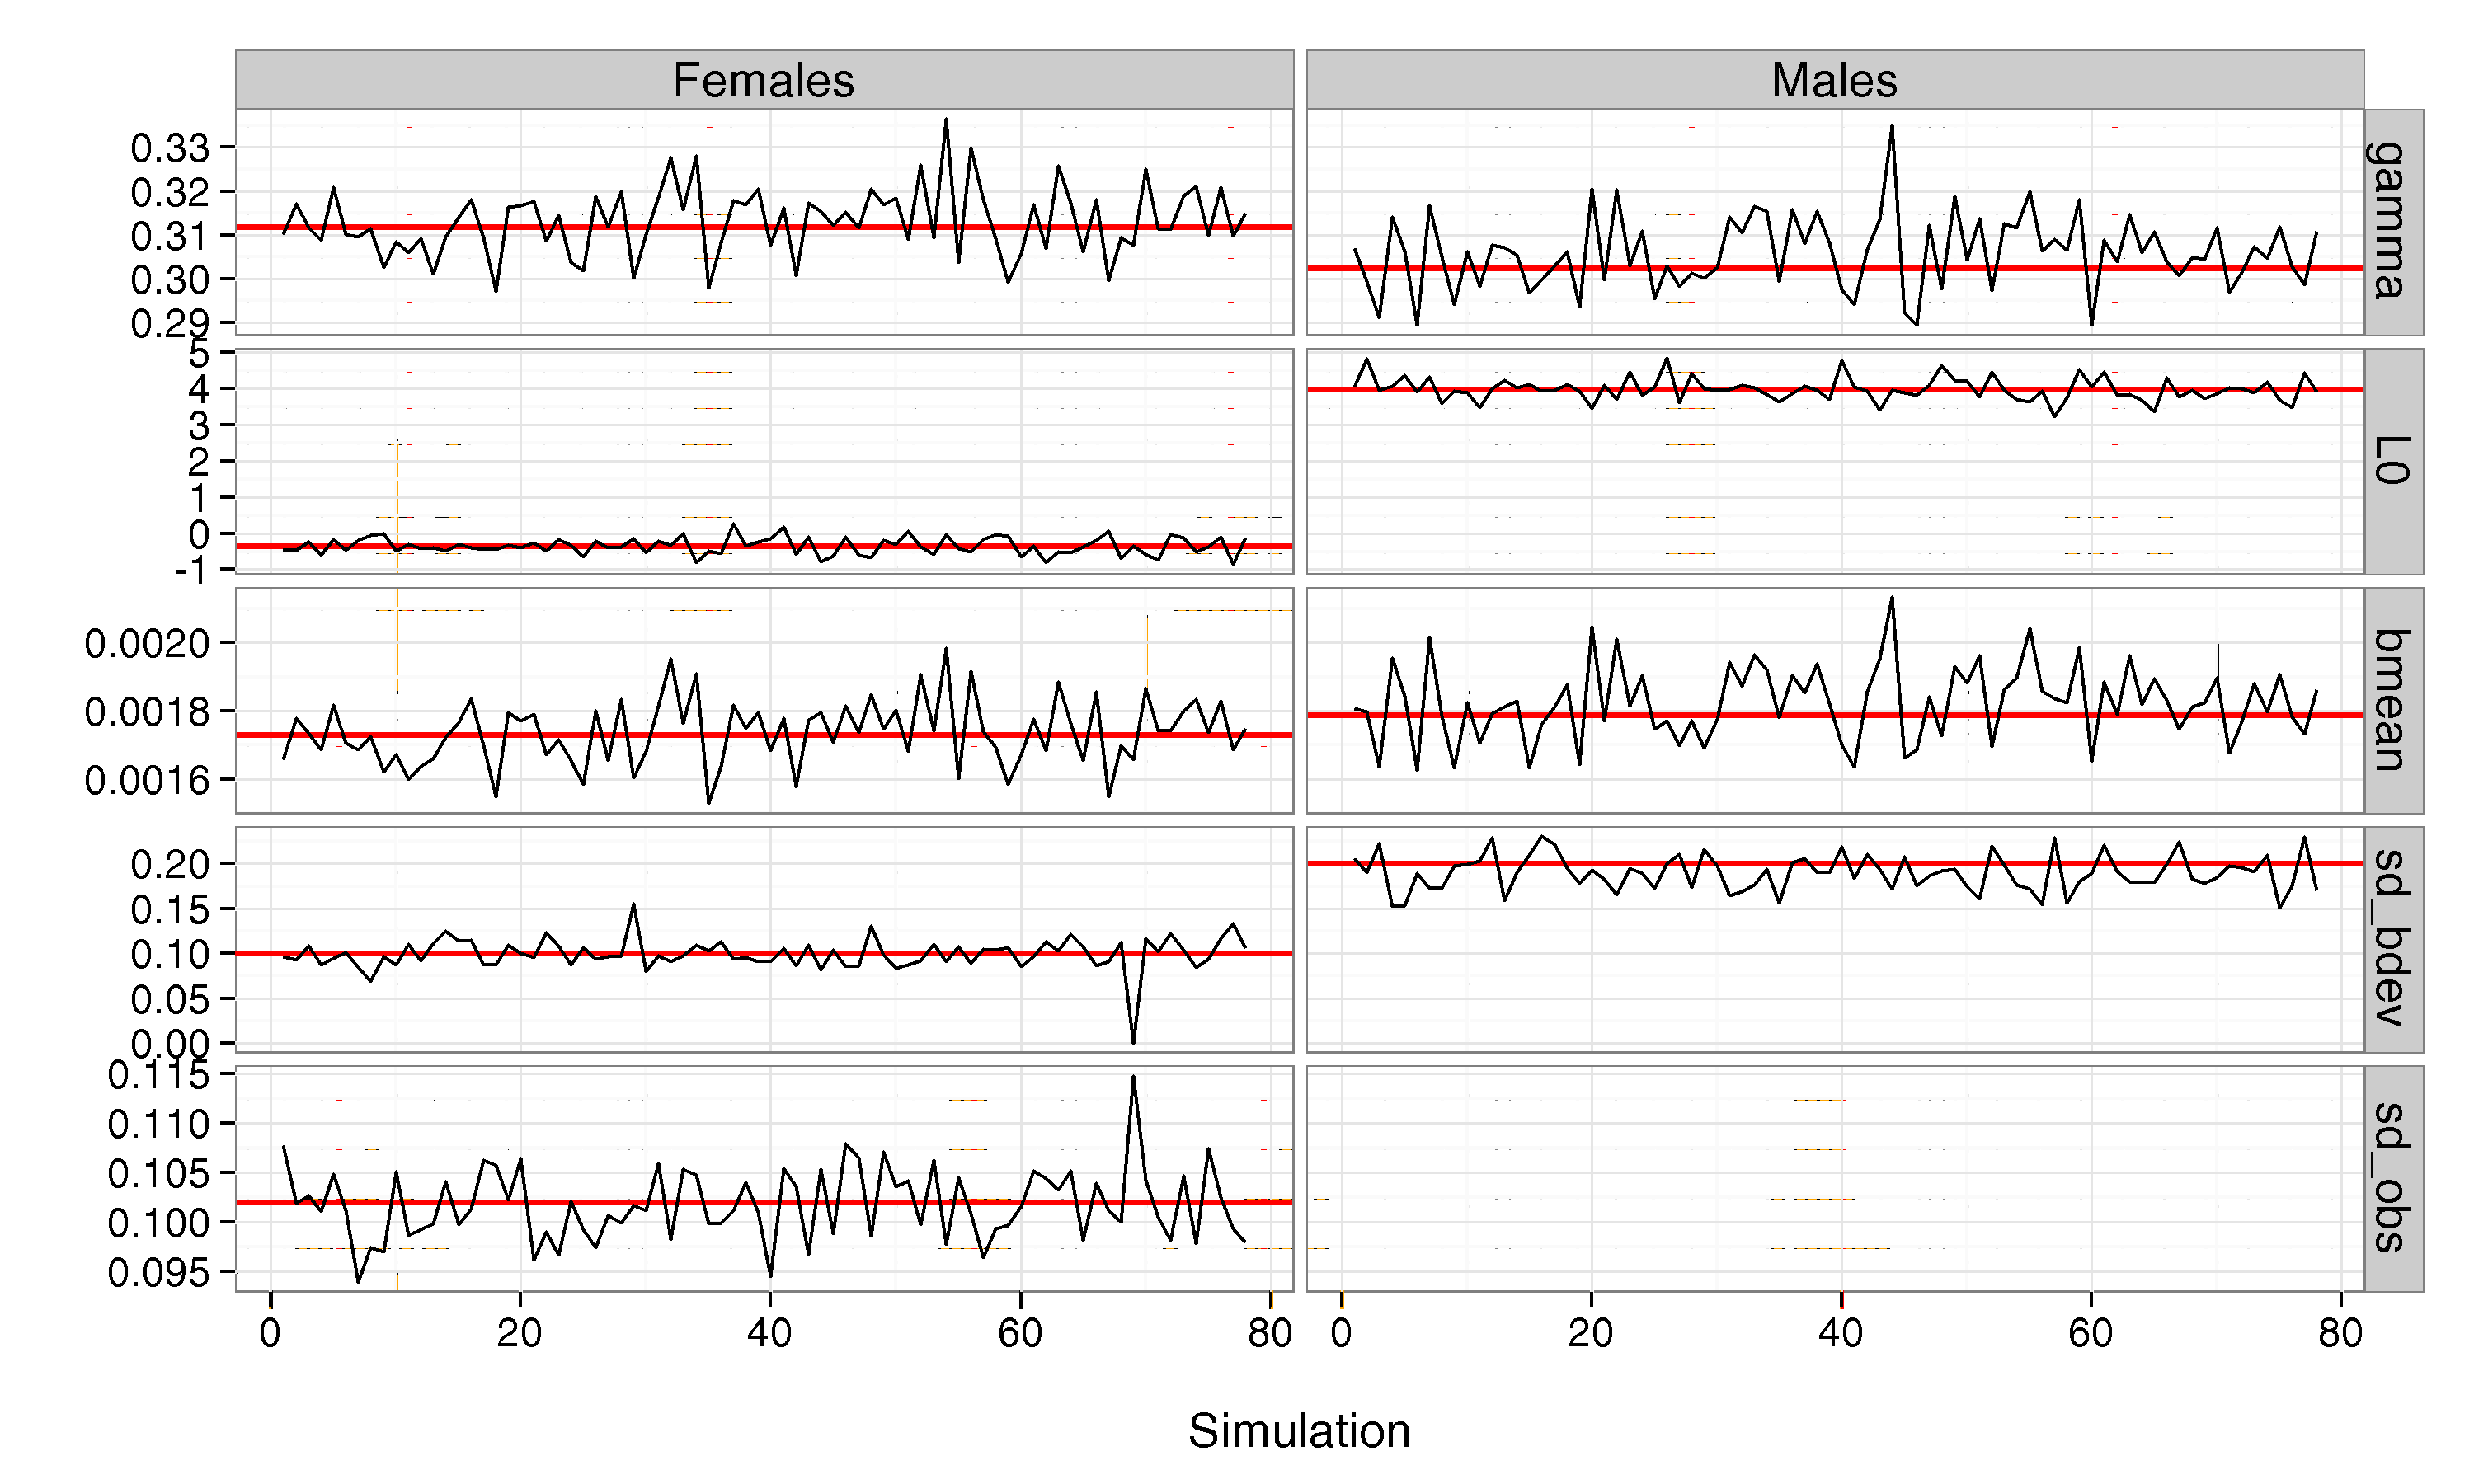
\includegraphics[width=\linewidth]{../simulation/v1/results/TracePars.png}
  \begin{quote}
    \caption{pdH fits plotted only.}
    \label{fig:sims1}
  \end{quote}
\end{figure}

%%%%%%%%%%%%%%%%%%%%%%%%%%%%%%%%%%%%%%%%%%%%%%%%%%%%%%%%%%%%%%%%%%%%%%%%%%%%%%%%%
\newpage\clearpage
\subsubsection{v2}
%%%%%%%%%%%%%%%%%%%%%%%%%%%%%%%%%%%%%%%%%%%%%%%%%%%%%%%%%%%%%%%%%%%%%%%%%%%%%%%%%
Random effects $z$, 92/100 pdH. Unfortunately I f'ed the estimation of this
model up and estimated a single sdz param but simulated two. I'll need to redo
the estimation here.

\begin{figure}[!htbp]
  \centering
  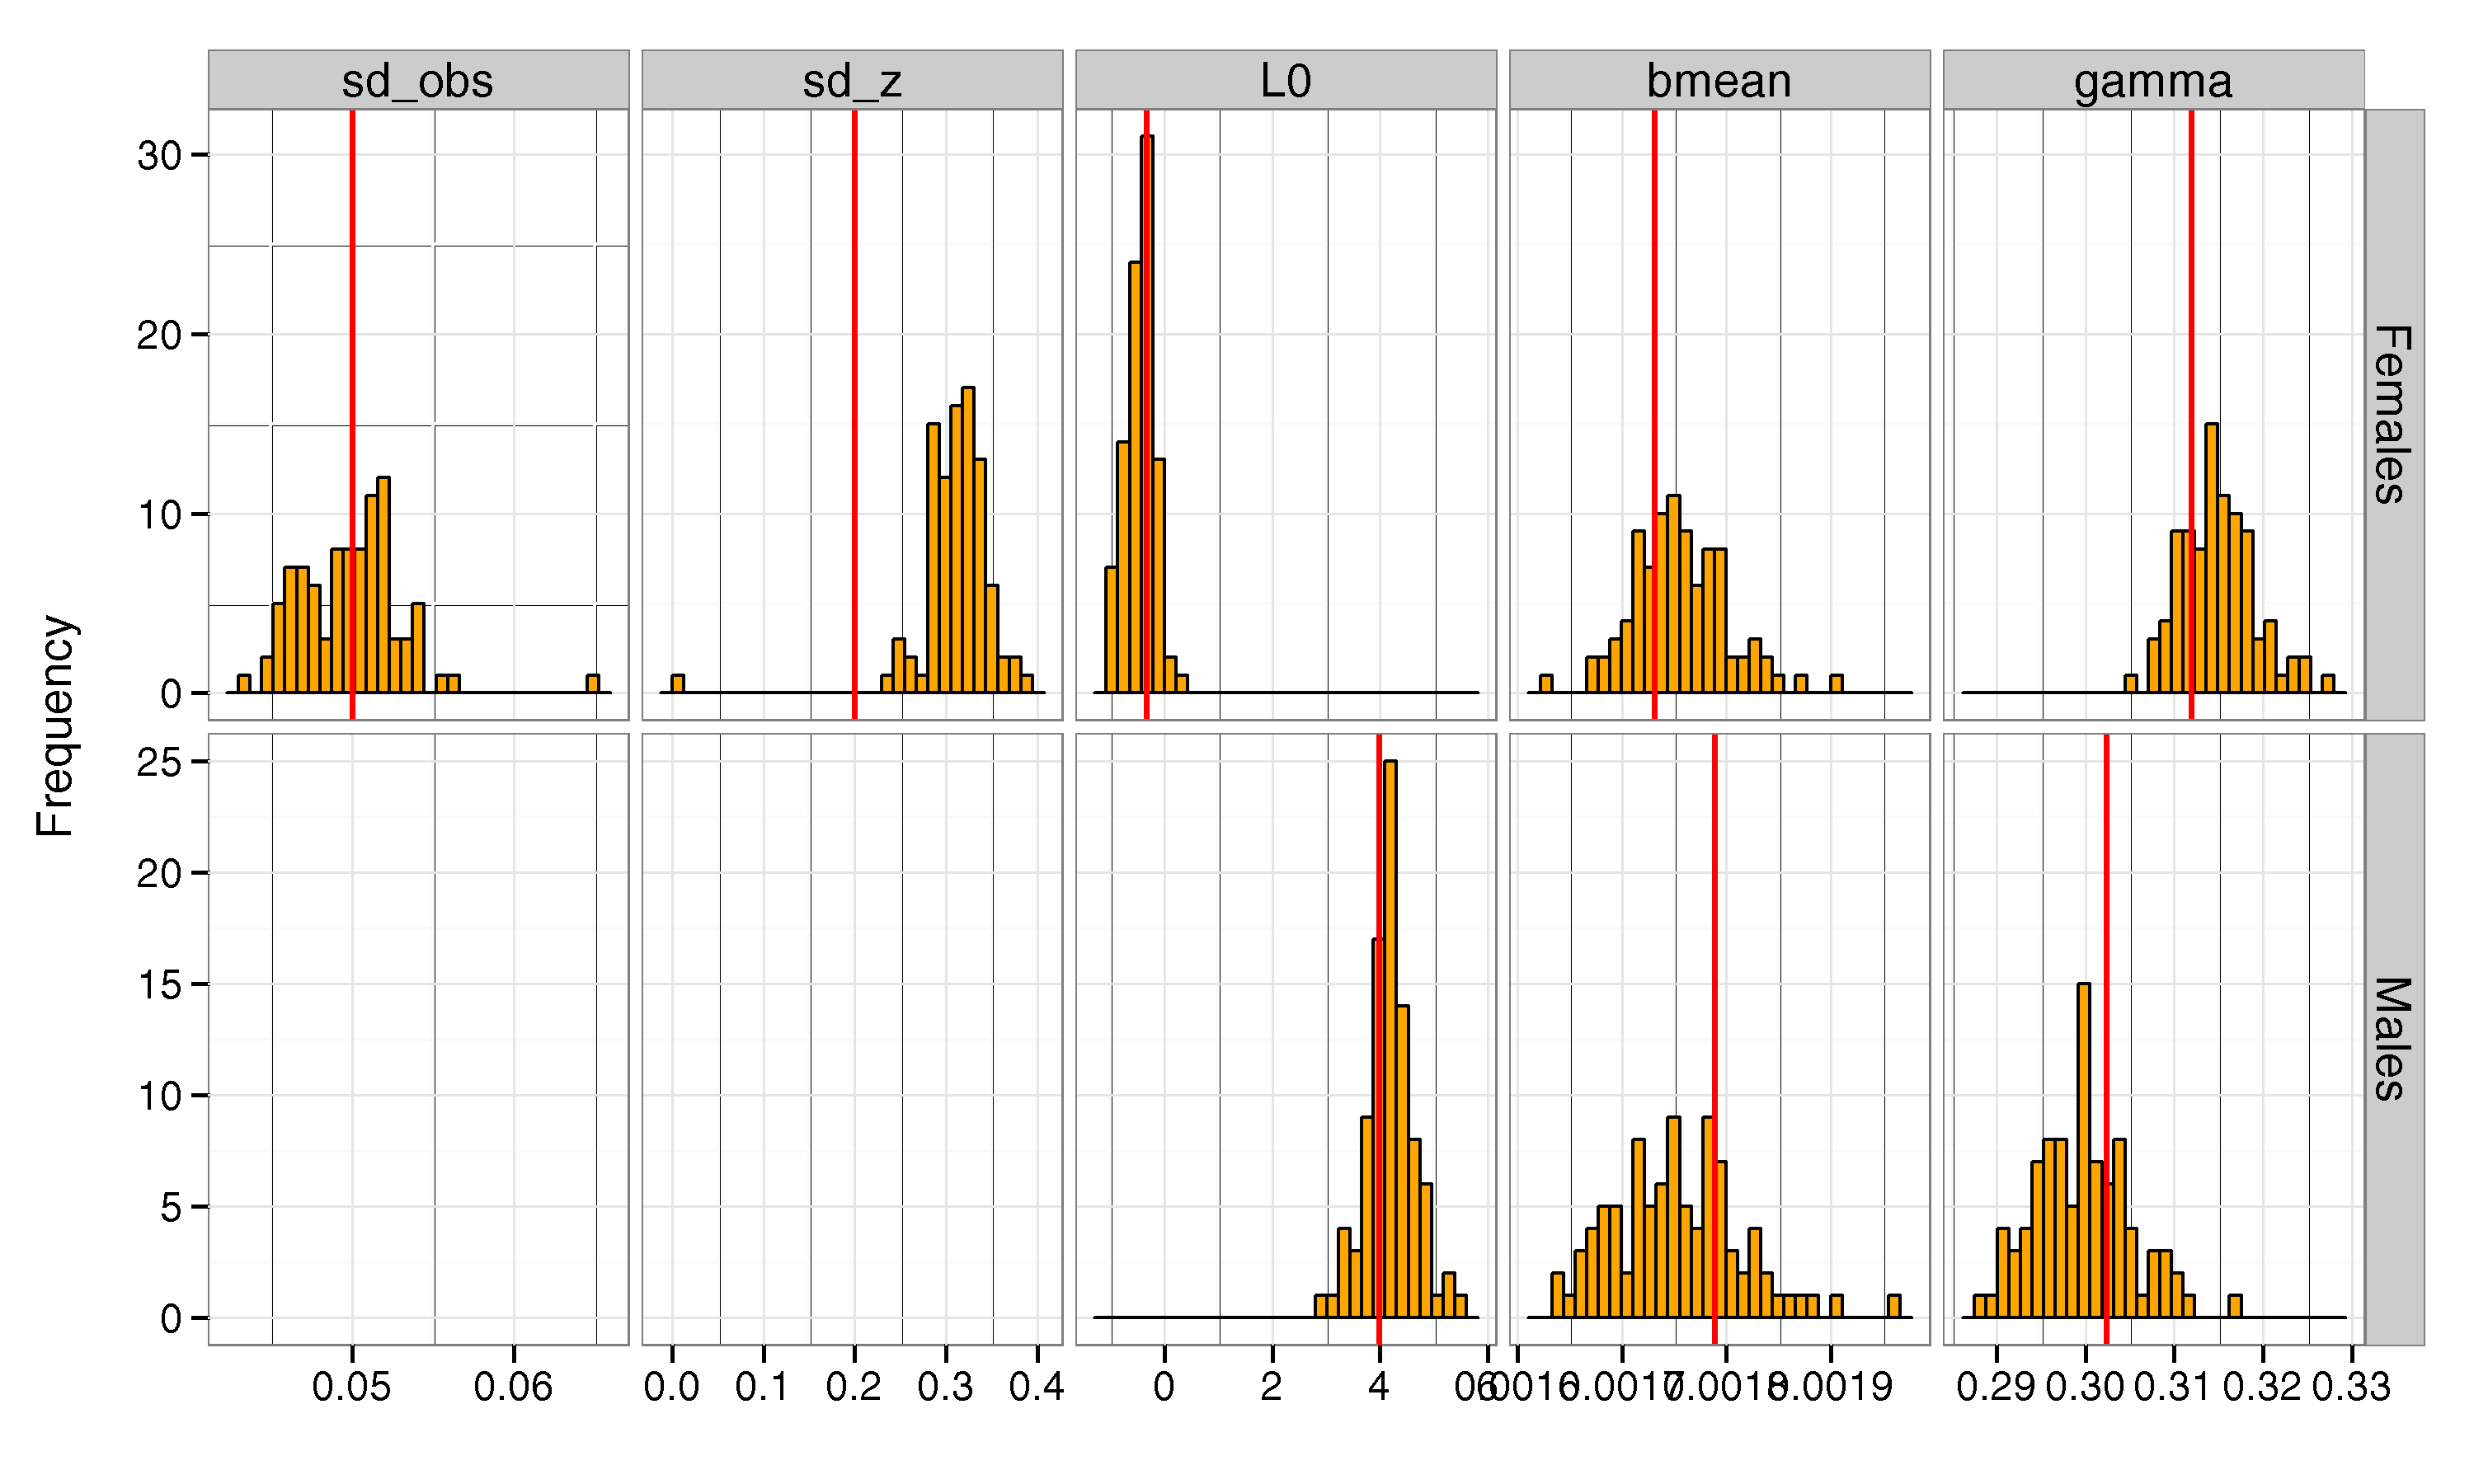
\includegraphics[width=\linewidth]{../simulation/v2/results/SimPars.png}
  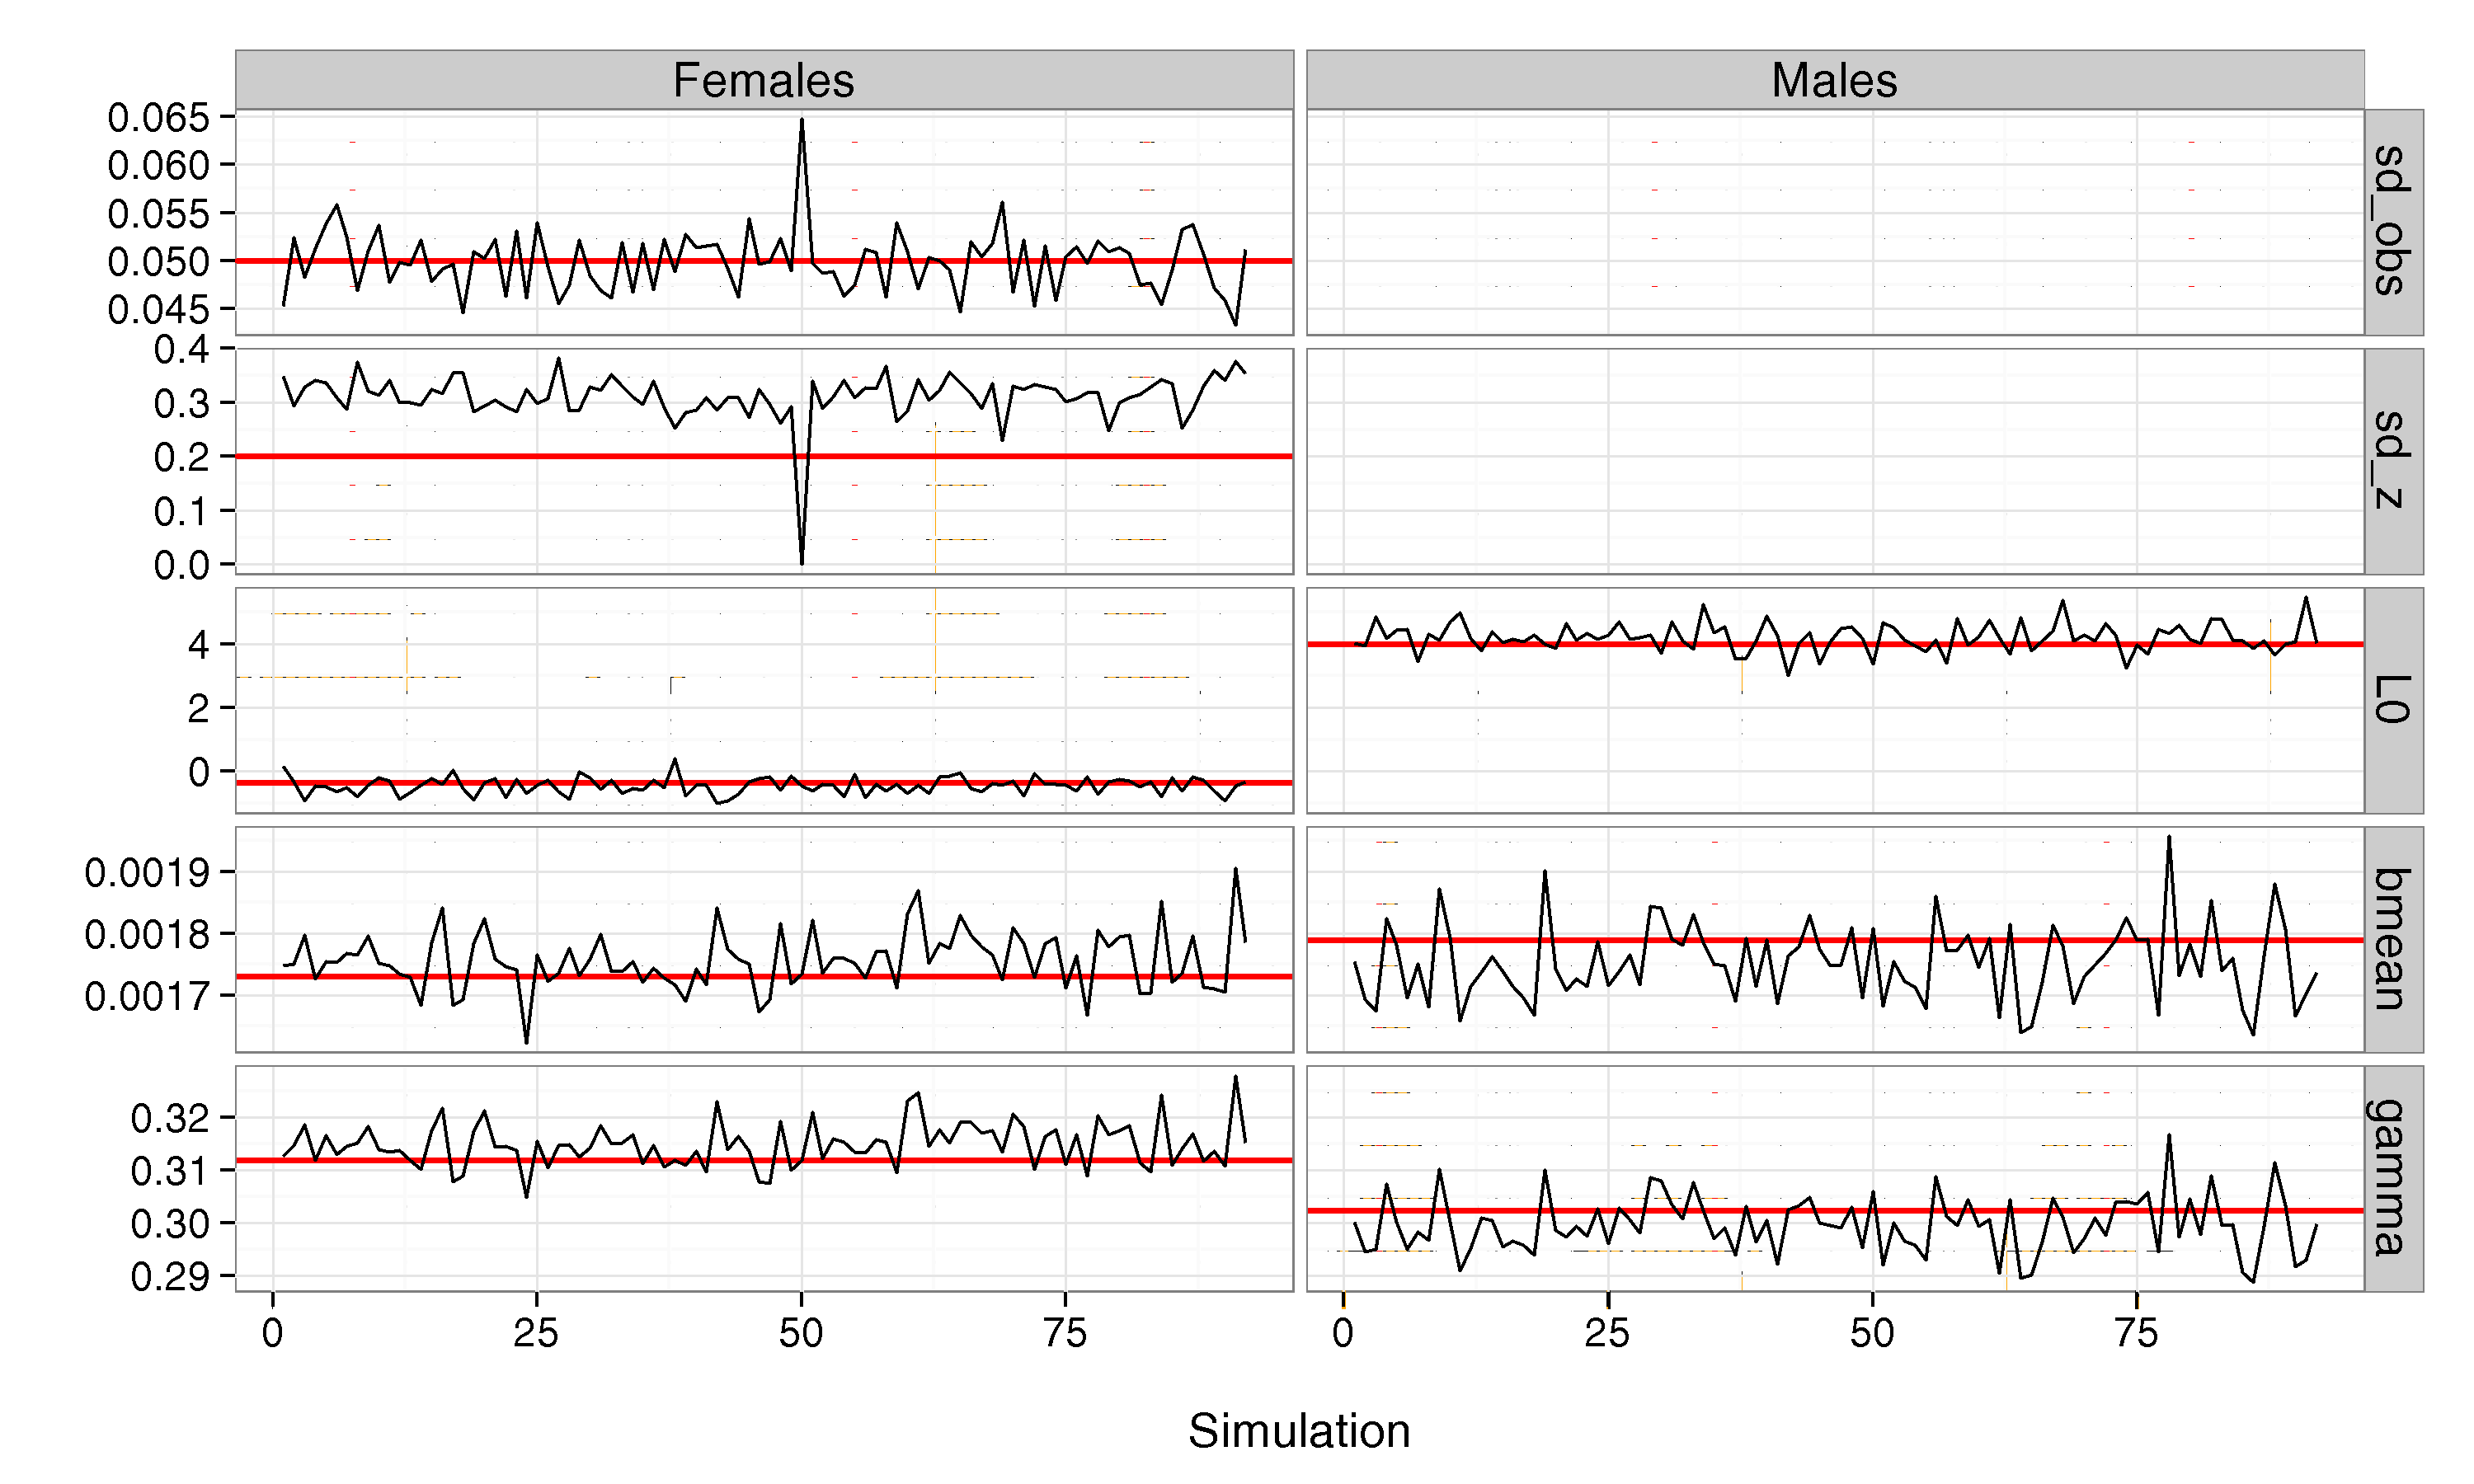
\includegraphics[width=\linewidth]{../simulation/v2/results/TracePars.png}
  \begin{quote}
    \caption{pdH fits plotted only.}
    \label{fig:sims1}
  \end{quote}
\end{figure}

%%%%%%%%%%%%%%%%%%%%%%%%%%%%%%%%%%%%%%%%%%%%%%%%%%%%%%%%%%%%%%%%%%%%%%%%%%%%%%%%%
\newpage\clearpage
\subsubsection{v3}
%%%%%%%%%%%%%%%%%%%%%%%%%%%%%%%%%%%%%%%%%%%%%%%%%%%%%%%%%%%%%%%%%%%%%%%%%%%%%%%%%
Random effects $k$ and $z$, 81/100 pdH. Unfortunately I f'ed the estimation of this
model up and estimated a single sdz param but simulated two. I'll need to redo
the estimation here.

\begin{figure}[!htbp]
  \centering
  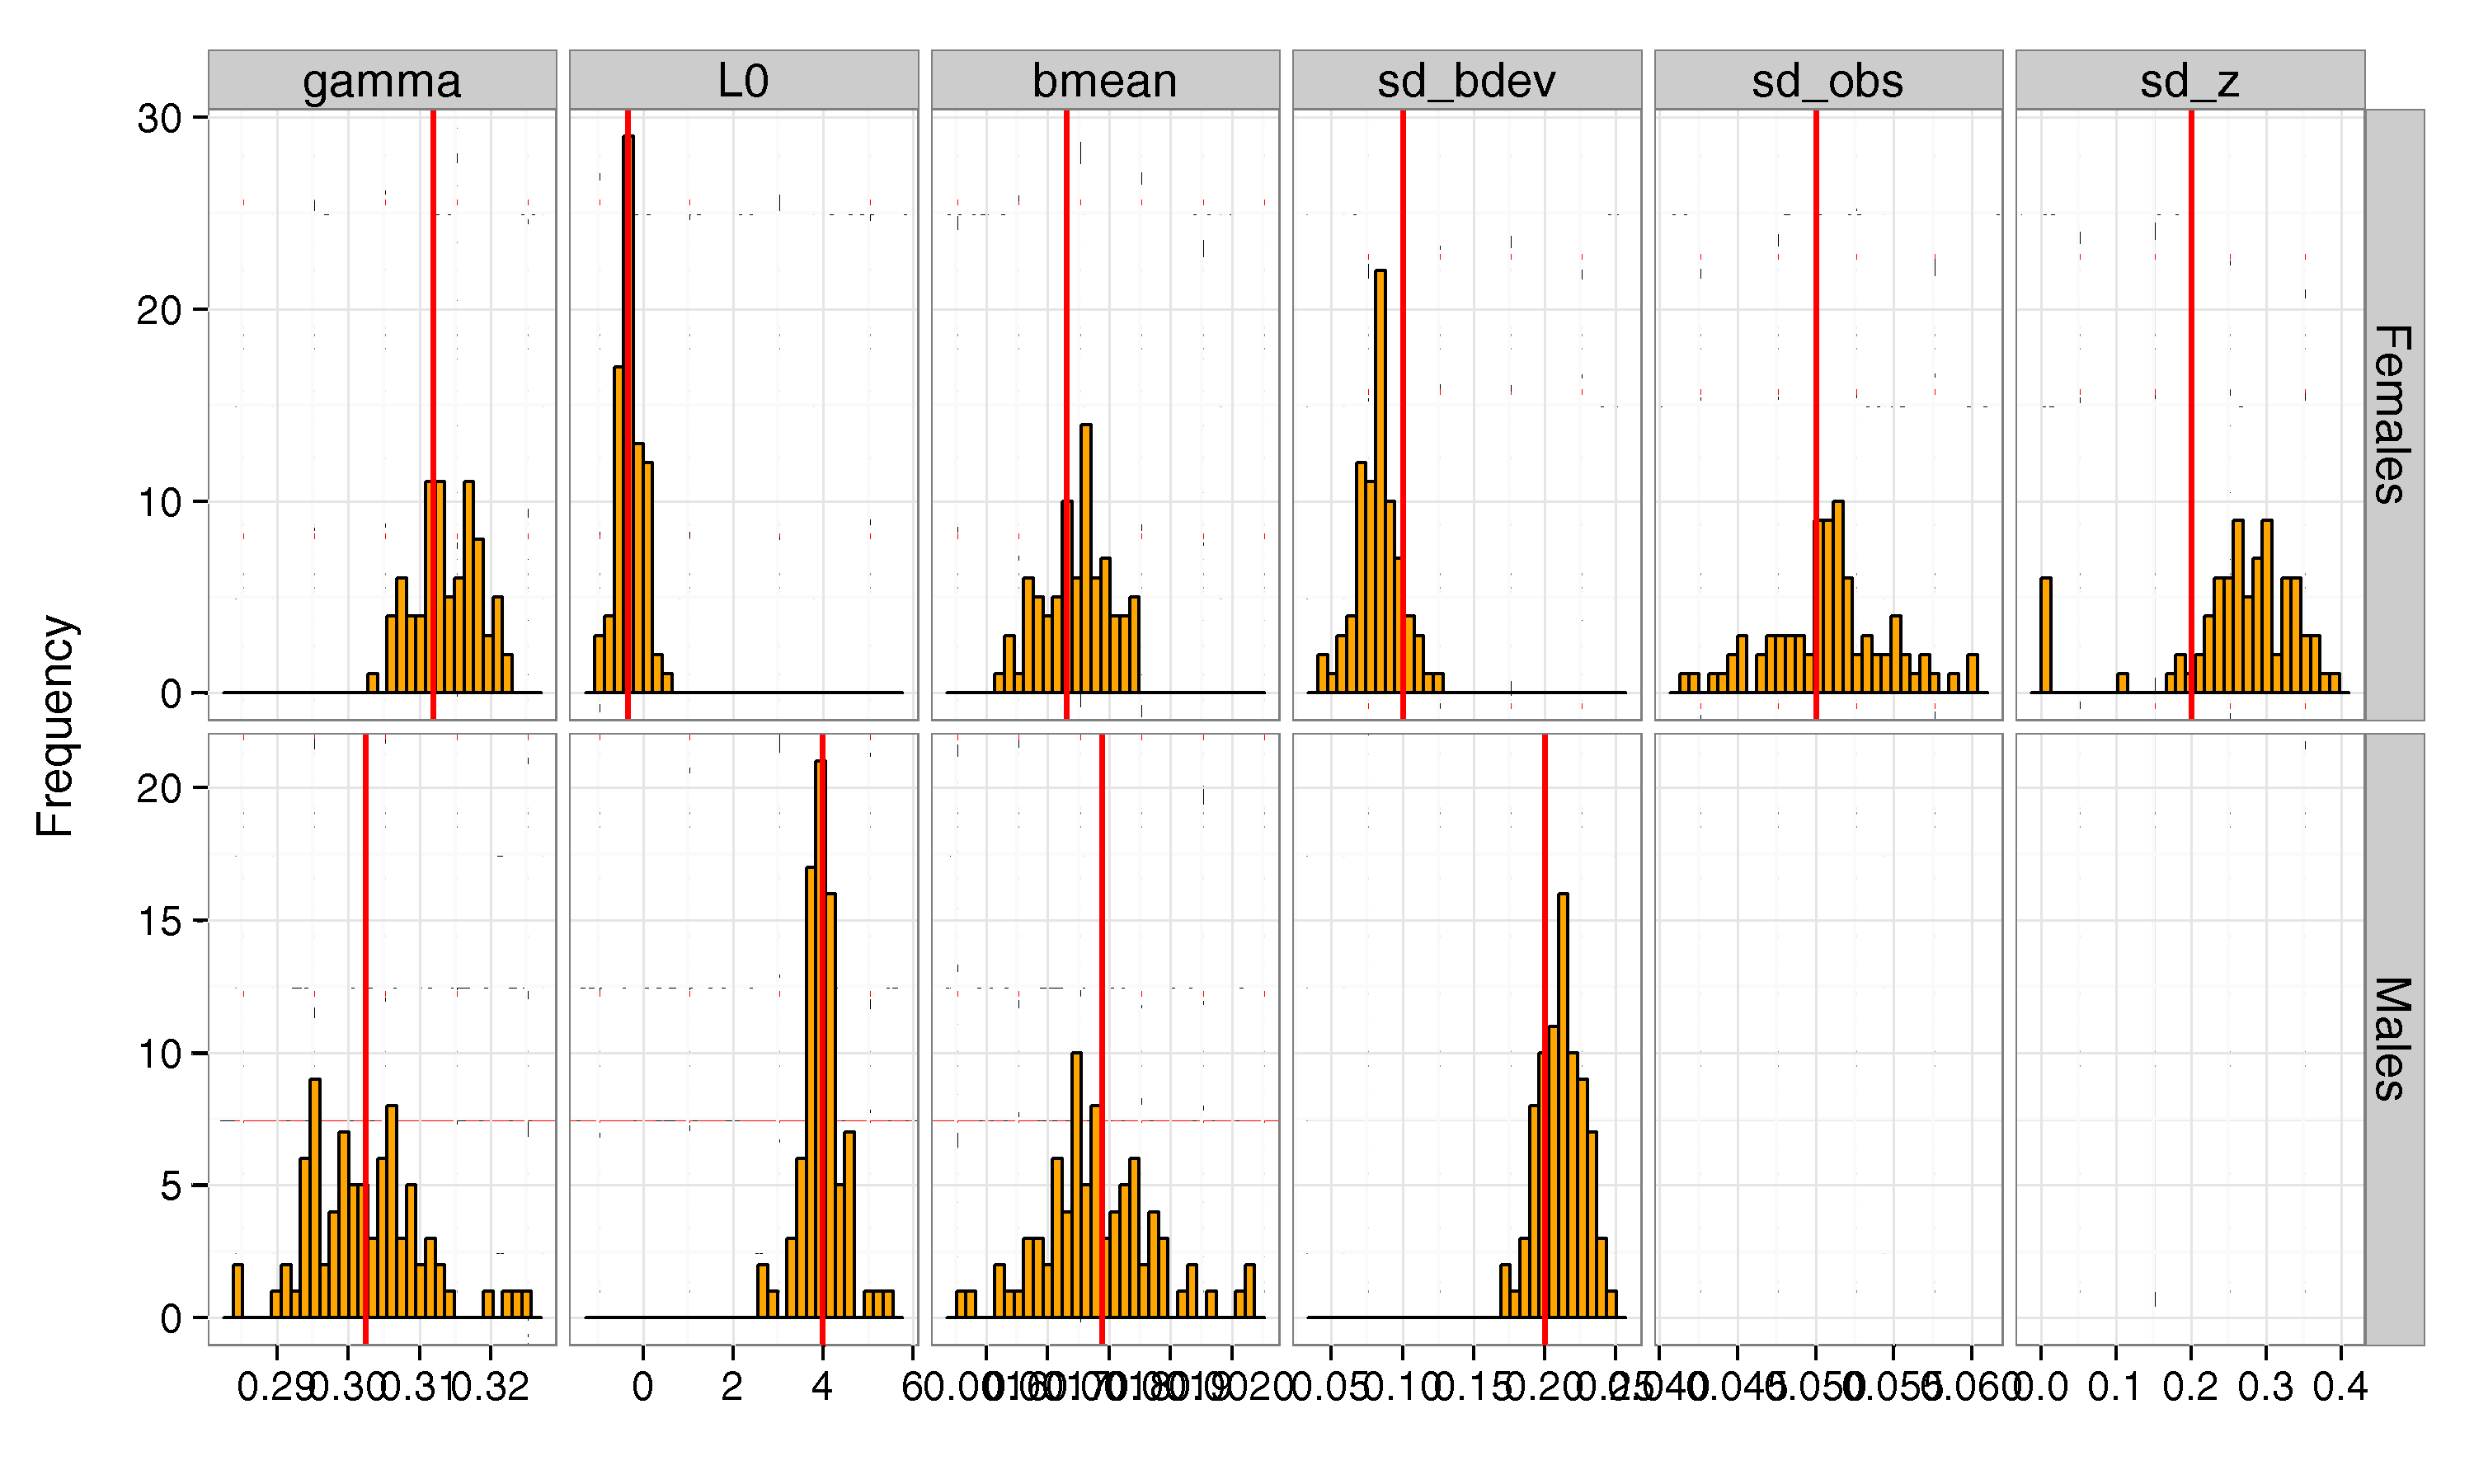
\includegraphics[width=\linewidth]{../simulation/v3/results/SimPars.png}
  \includegraphics[width=\linewidth]{../simulation/v3/results/TracePars.png}
  \begin{quote}
    \caption{pdH fits plotted only.}
    \label{fig:sims1}
  \end{quote}
\end{figure}







%%%%%%%%%%%%%%%%%%%%%%%%%%%%%%%%%%%%%%%%%%%%%%%%%%%%%%%%%%%%%%%%%%%%%%%%%%%%%%%%%

%\bibliographystyle{agsm}
%\bibliography{refs/myrefs}

%%%%%%%%%%%%%%%%%%%%%%%%%%%%%%%%%%%%%%%%%%%%%%%%%%%%%%%%%%%%%%%%%%%%%%%%%%%%%%%%%

\end{document}




I also tried this:
\begin{itemize}
\item Sampled sex using a binomial distribution.
\item Fit lognormal distributions to Age1 and time at liberty and simulate
  independently from the distributions.
\item Calculate Age2 given Age1 and time at liberty.
\item Rounded Age1, Age2 and time at liberty off to the nearest integer.
\end{itemize}
But this resulted in unrealistic Age2's (i.e. when a long time at liberty is
added to an already old fish), the plots just looked a bit silly.

Below are some exmaple plots using the first sampling approach above then
running these through our simulation model. 
\begin{figure}[!htbp]
  \centering
  %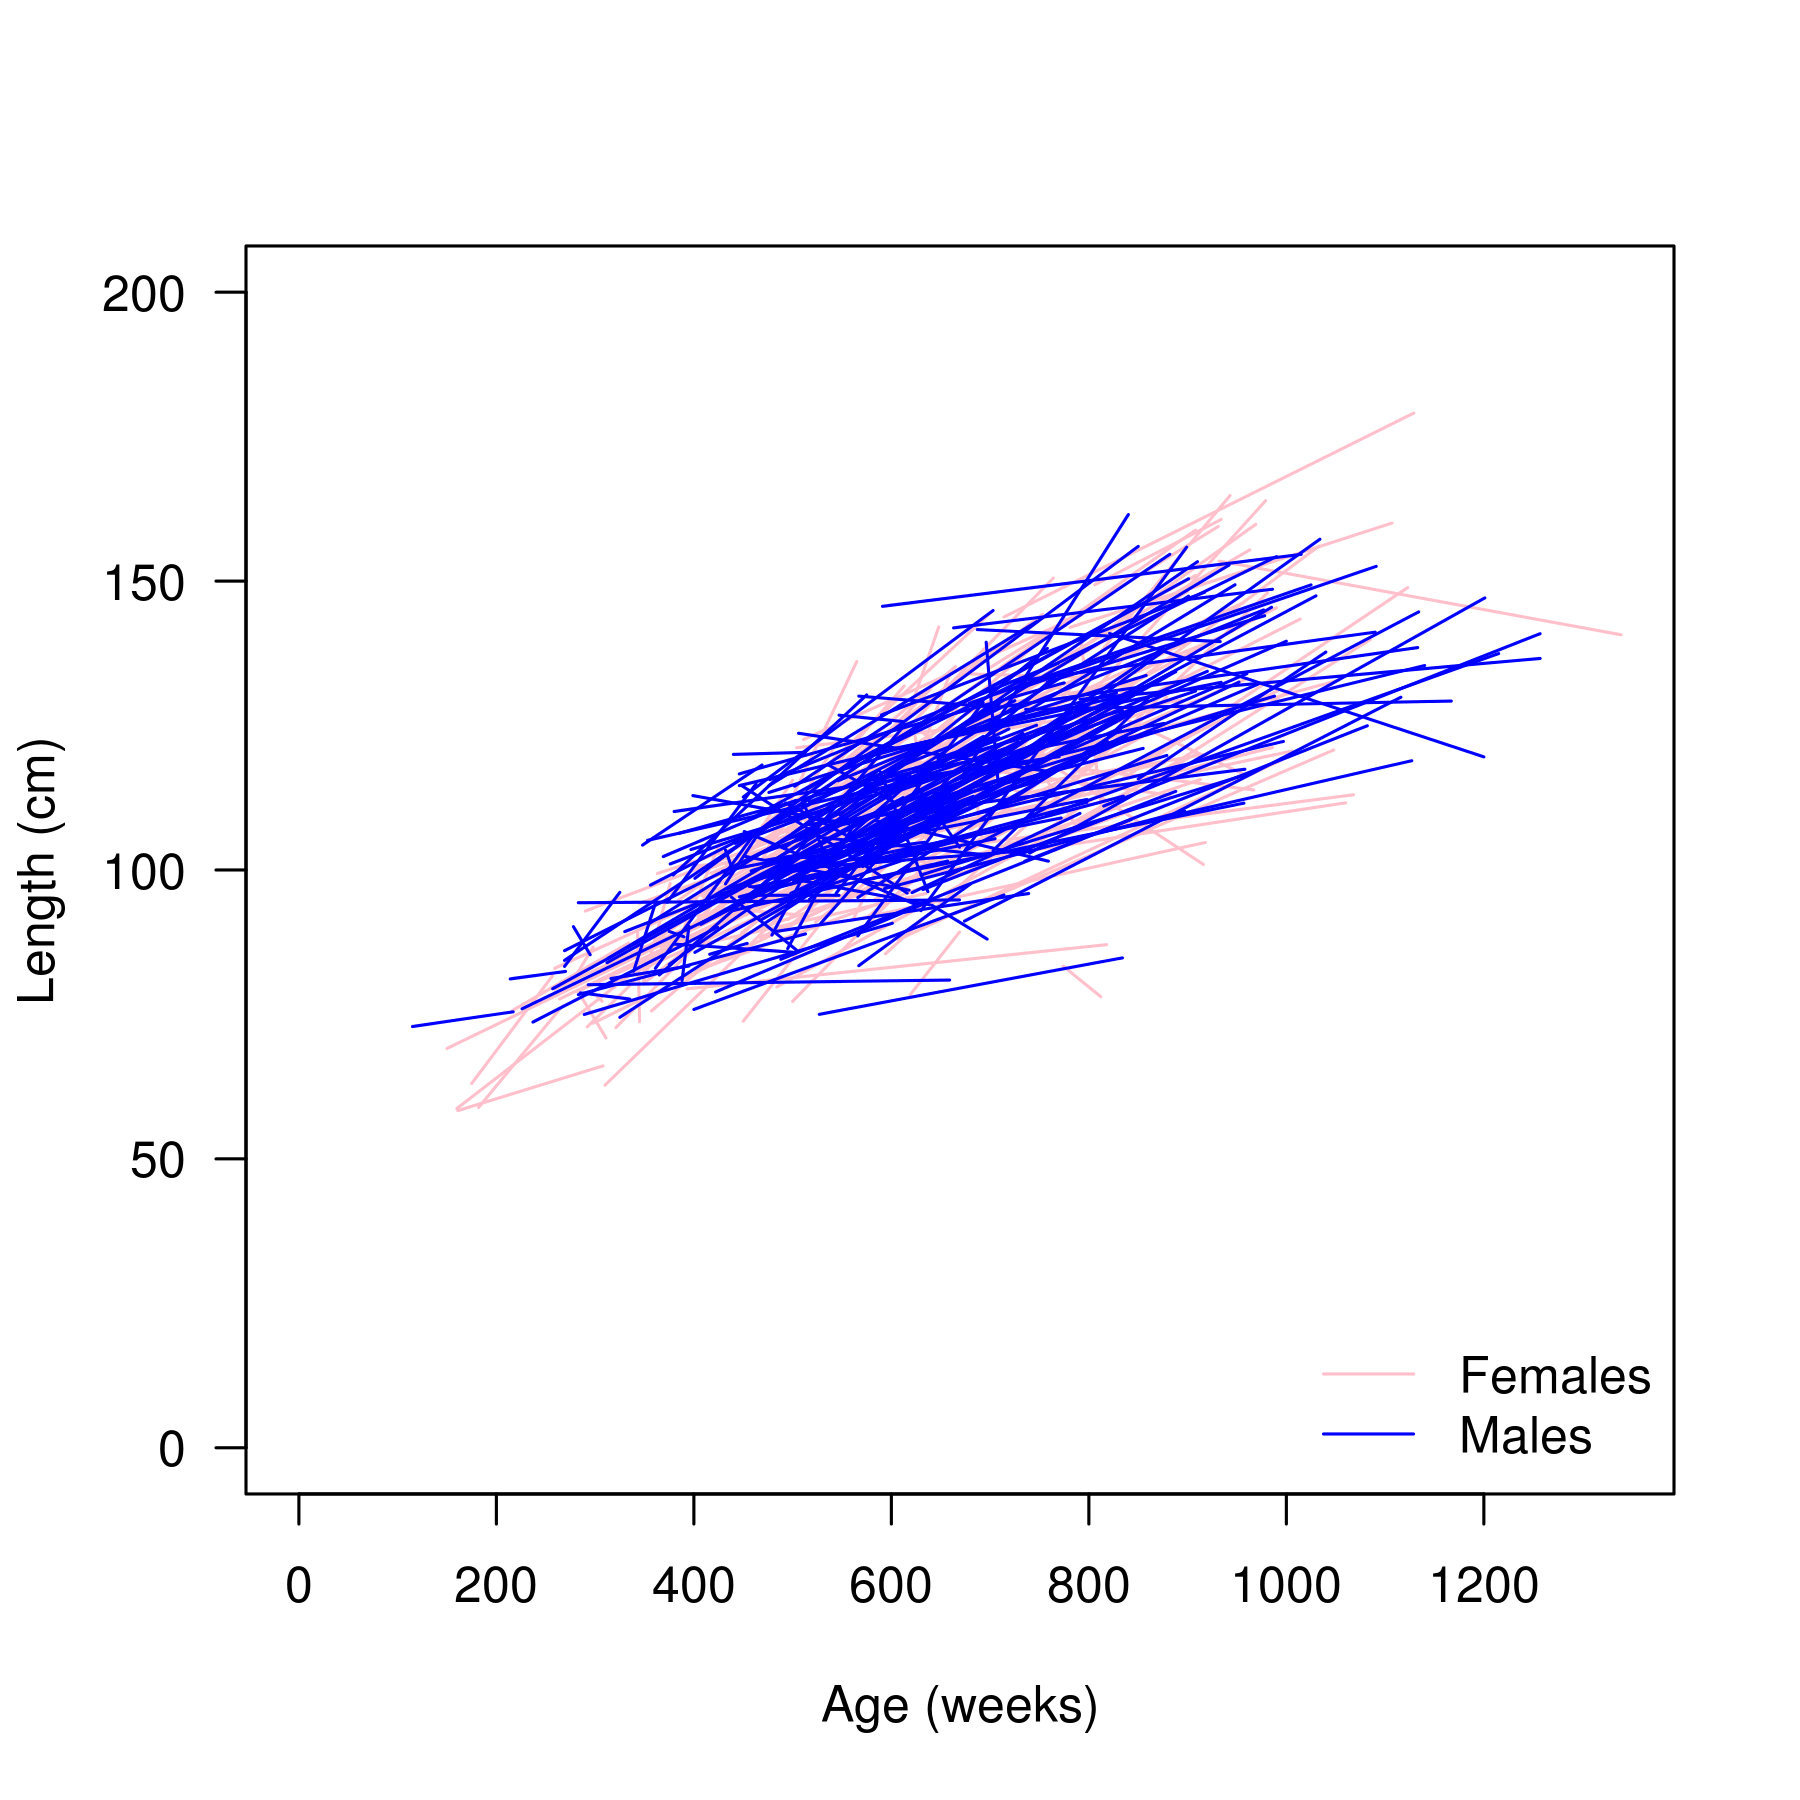
\includegraphics[width=0.49\linewidth]{../simulation/sims/growth-1.png}
  %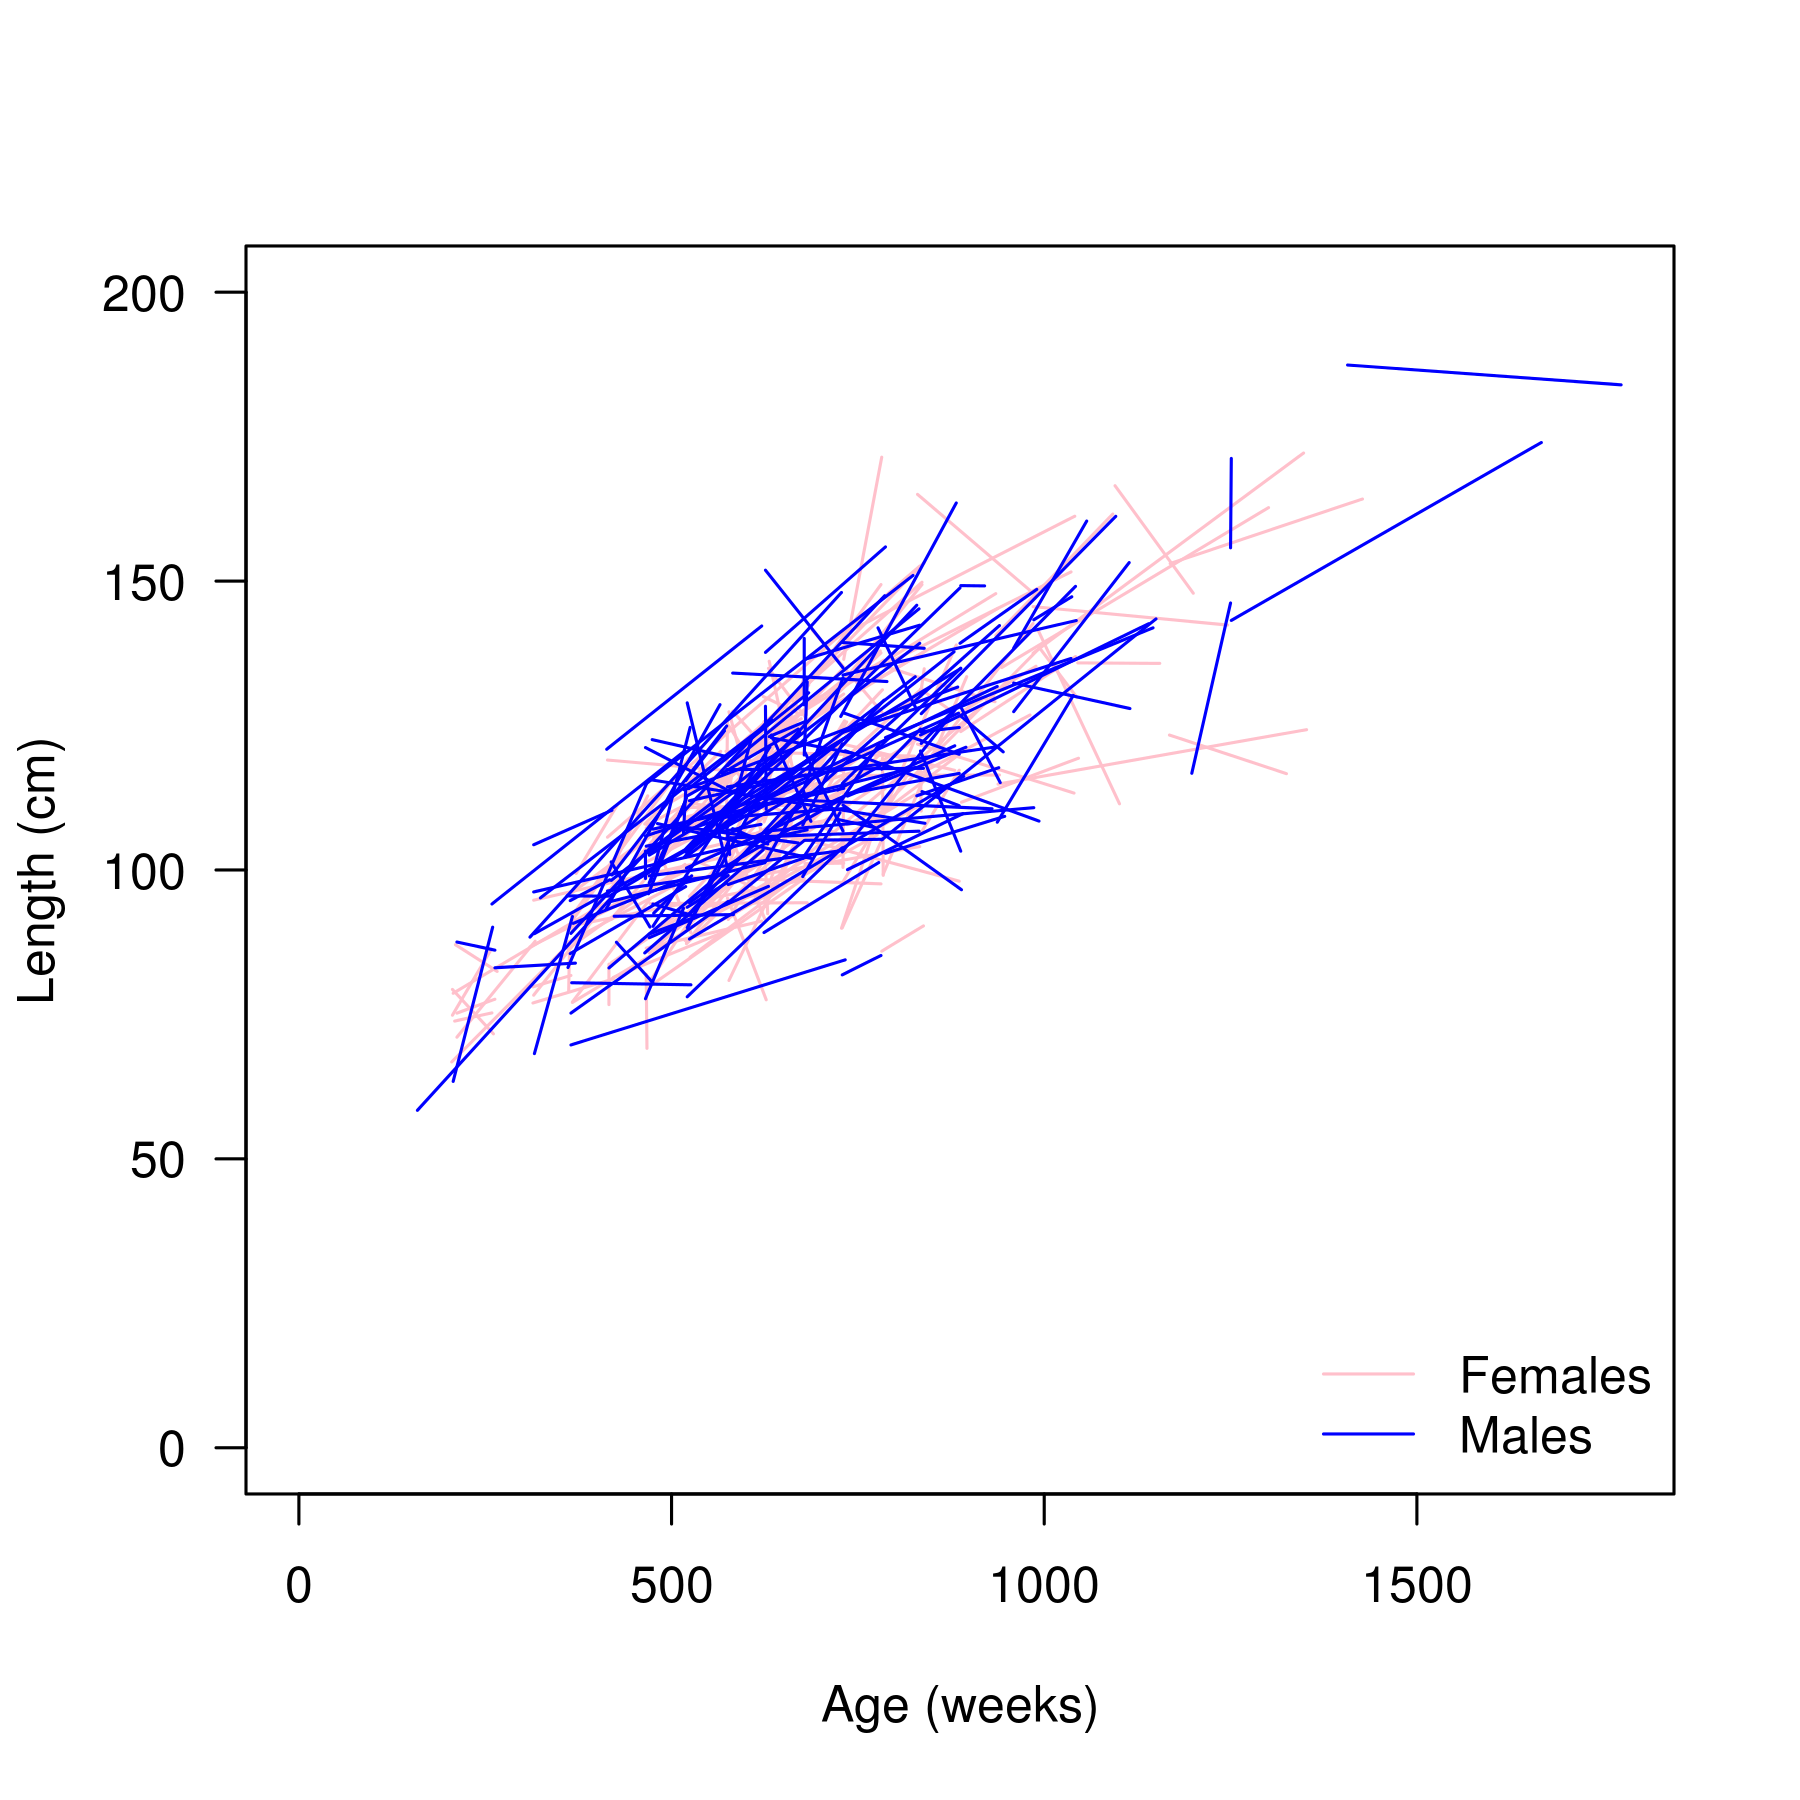
\includegraphics[width=0.49\linewidth]{../simulation/sims/growth-2.png}
  %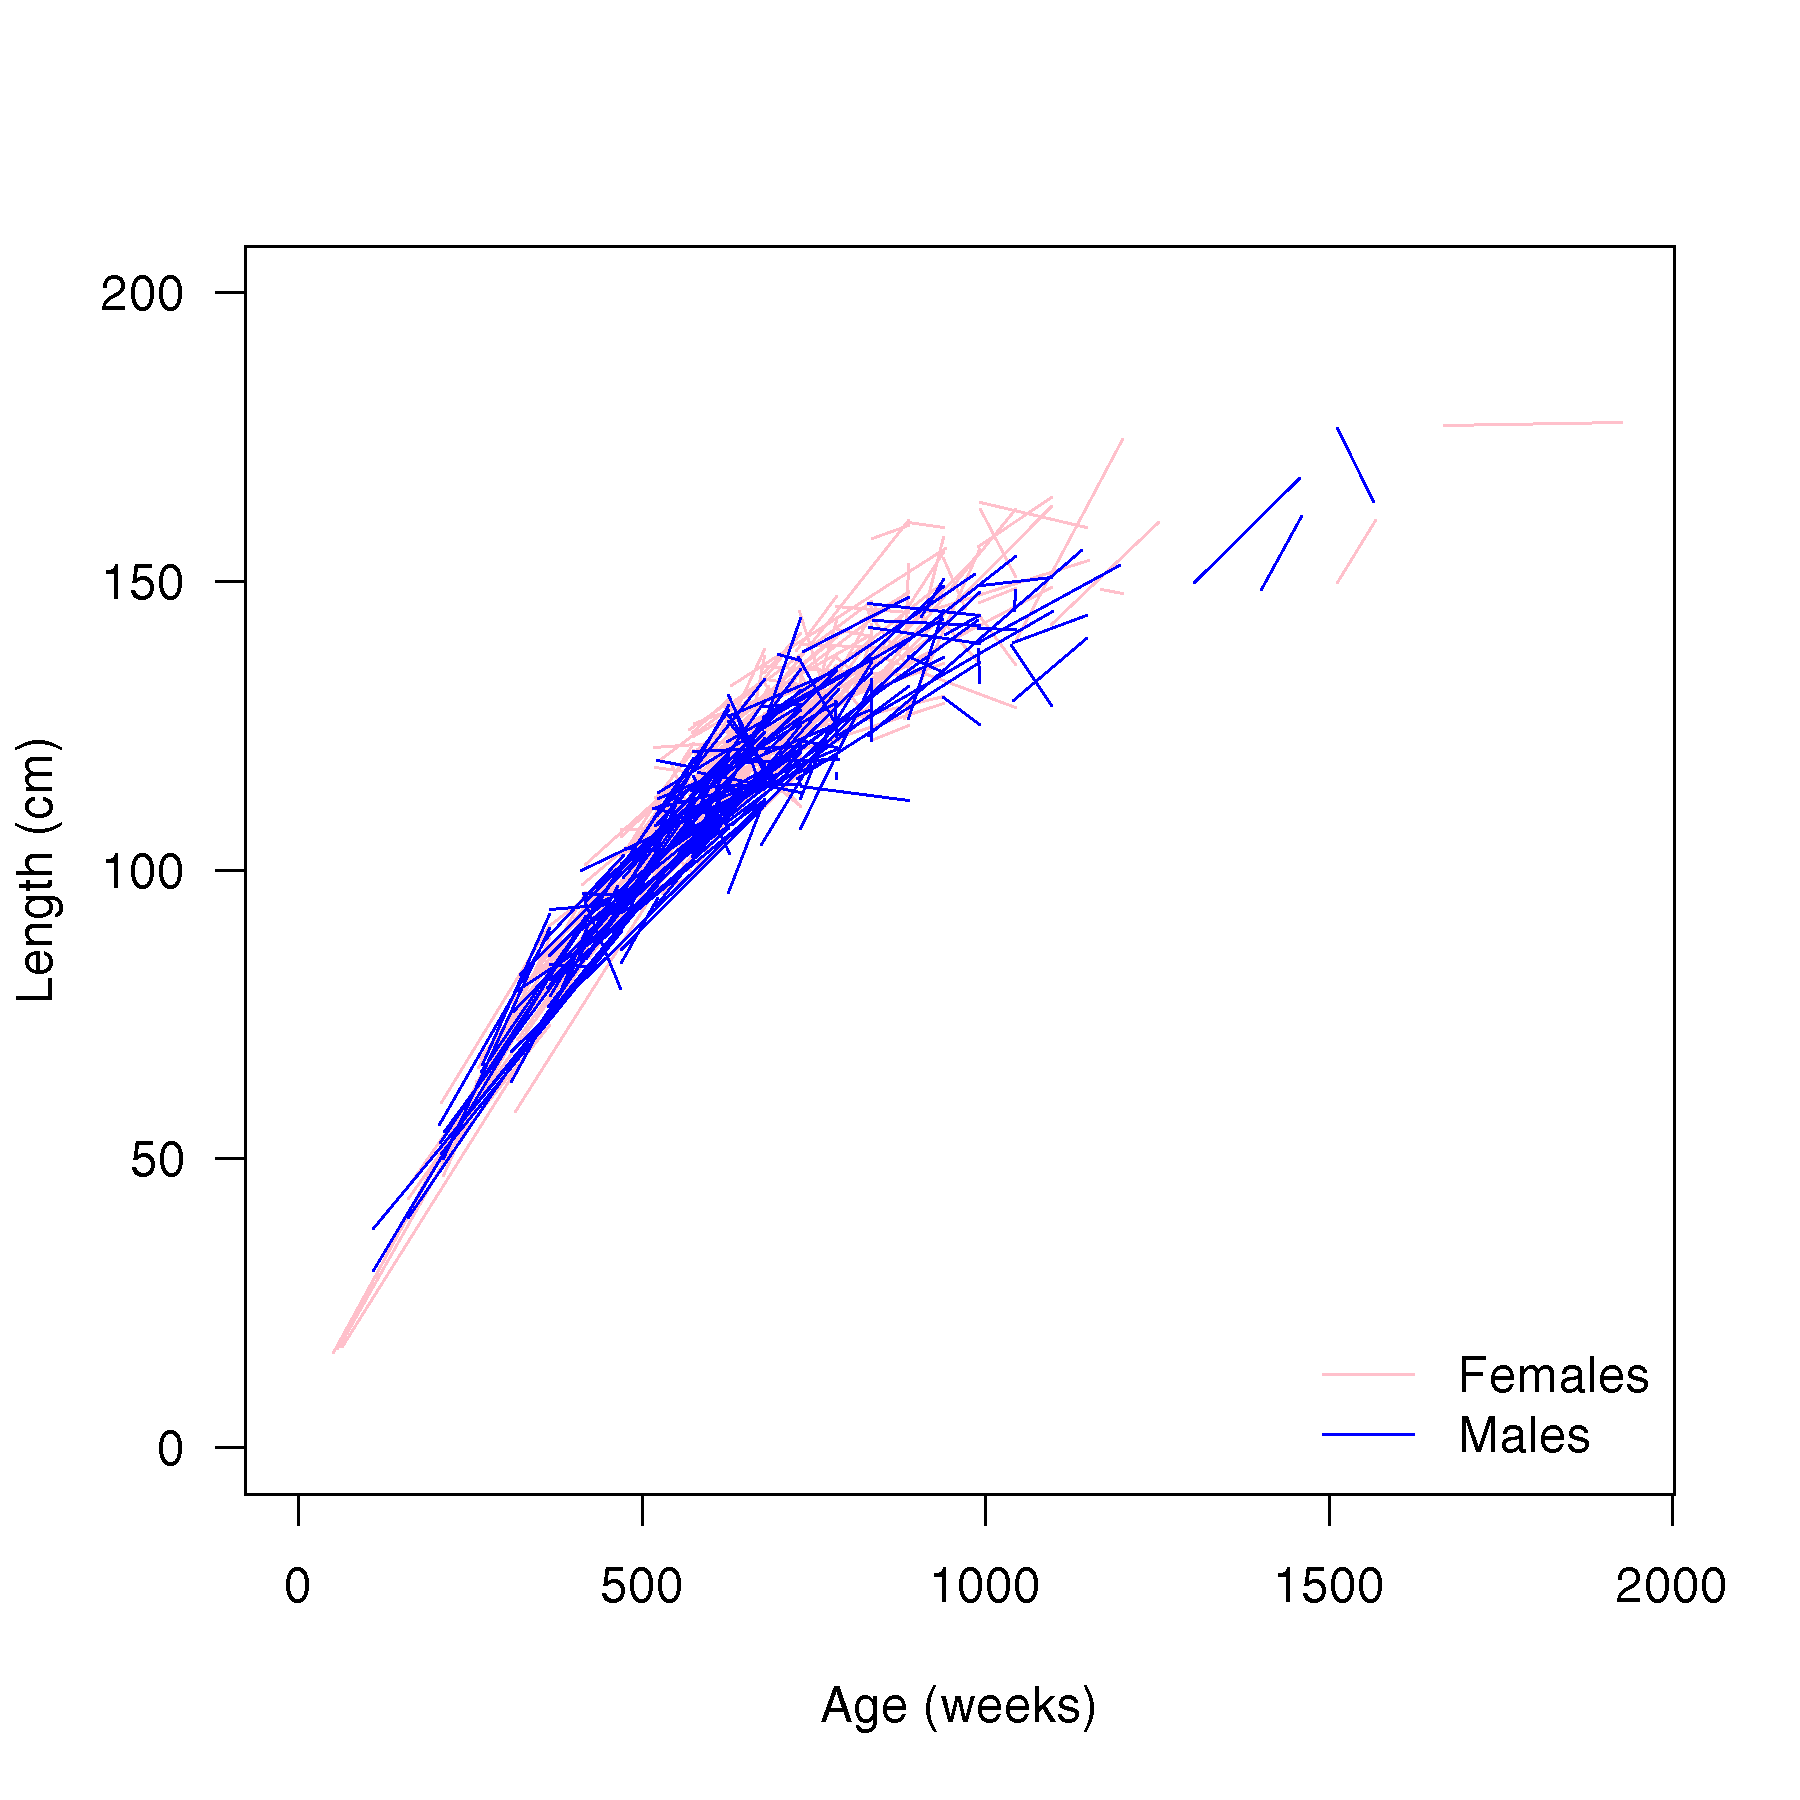
\includegraphics[width=0.49\linewidth]{../simulation/sims/growth-6.png}
  %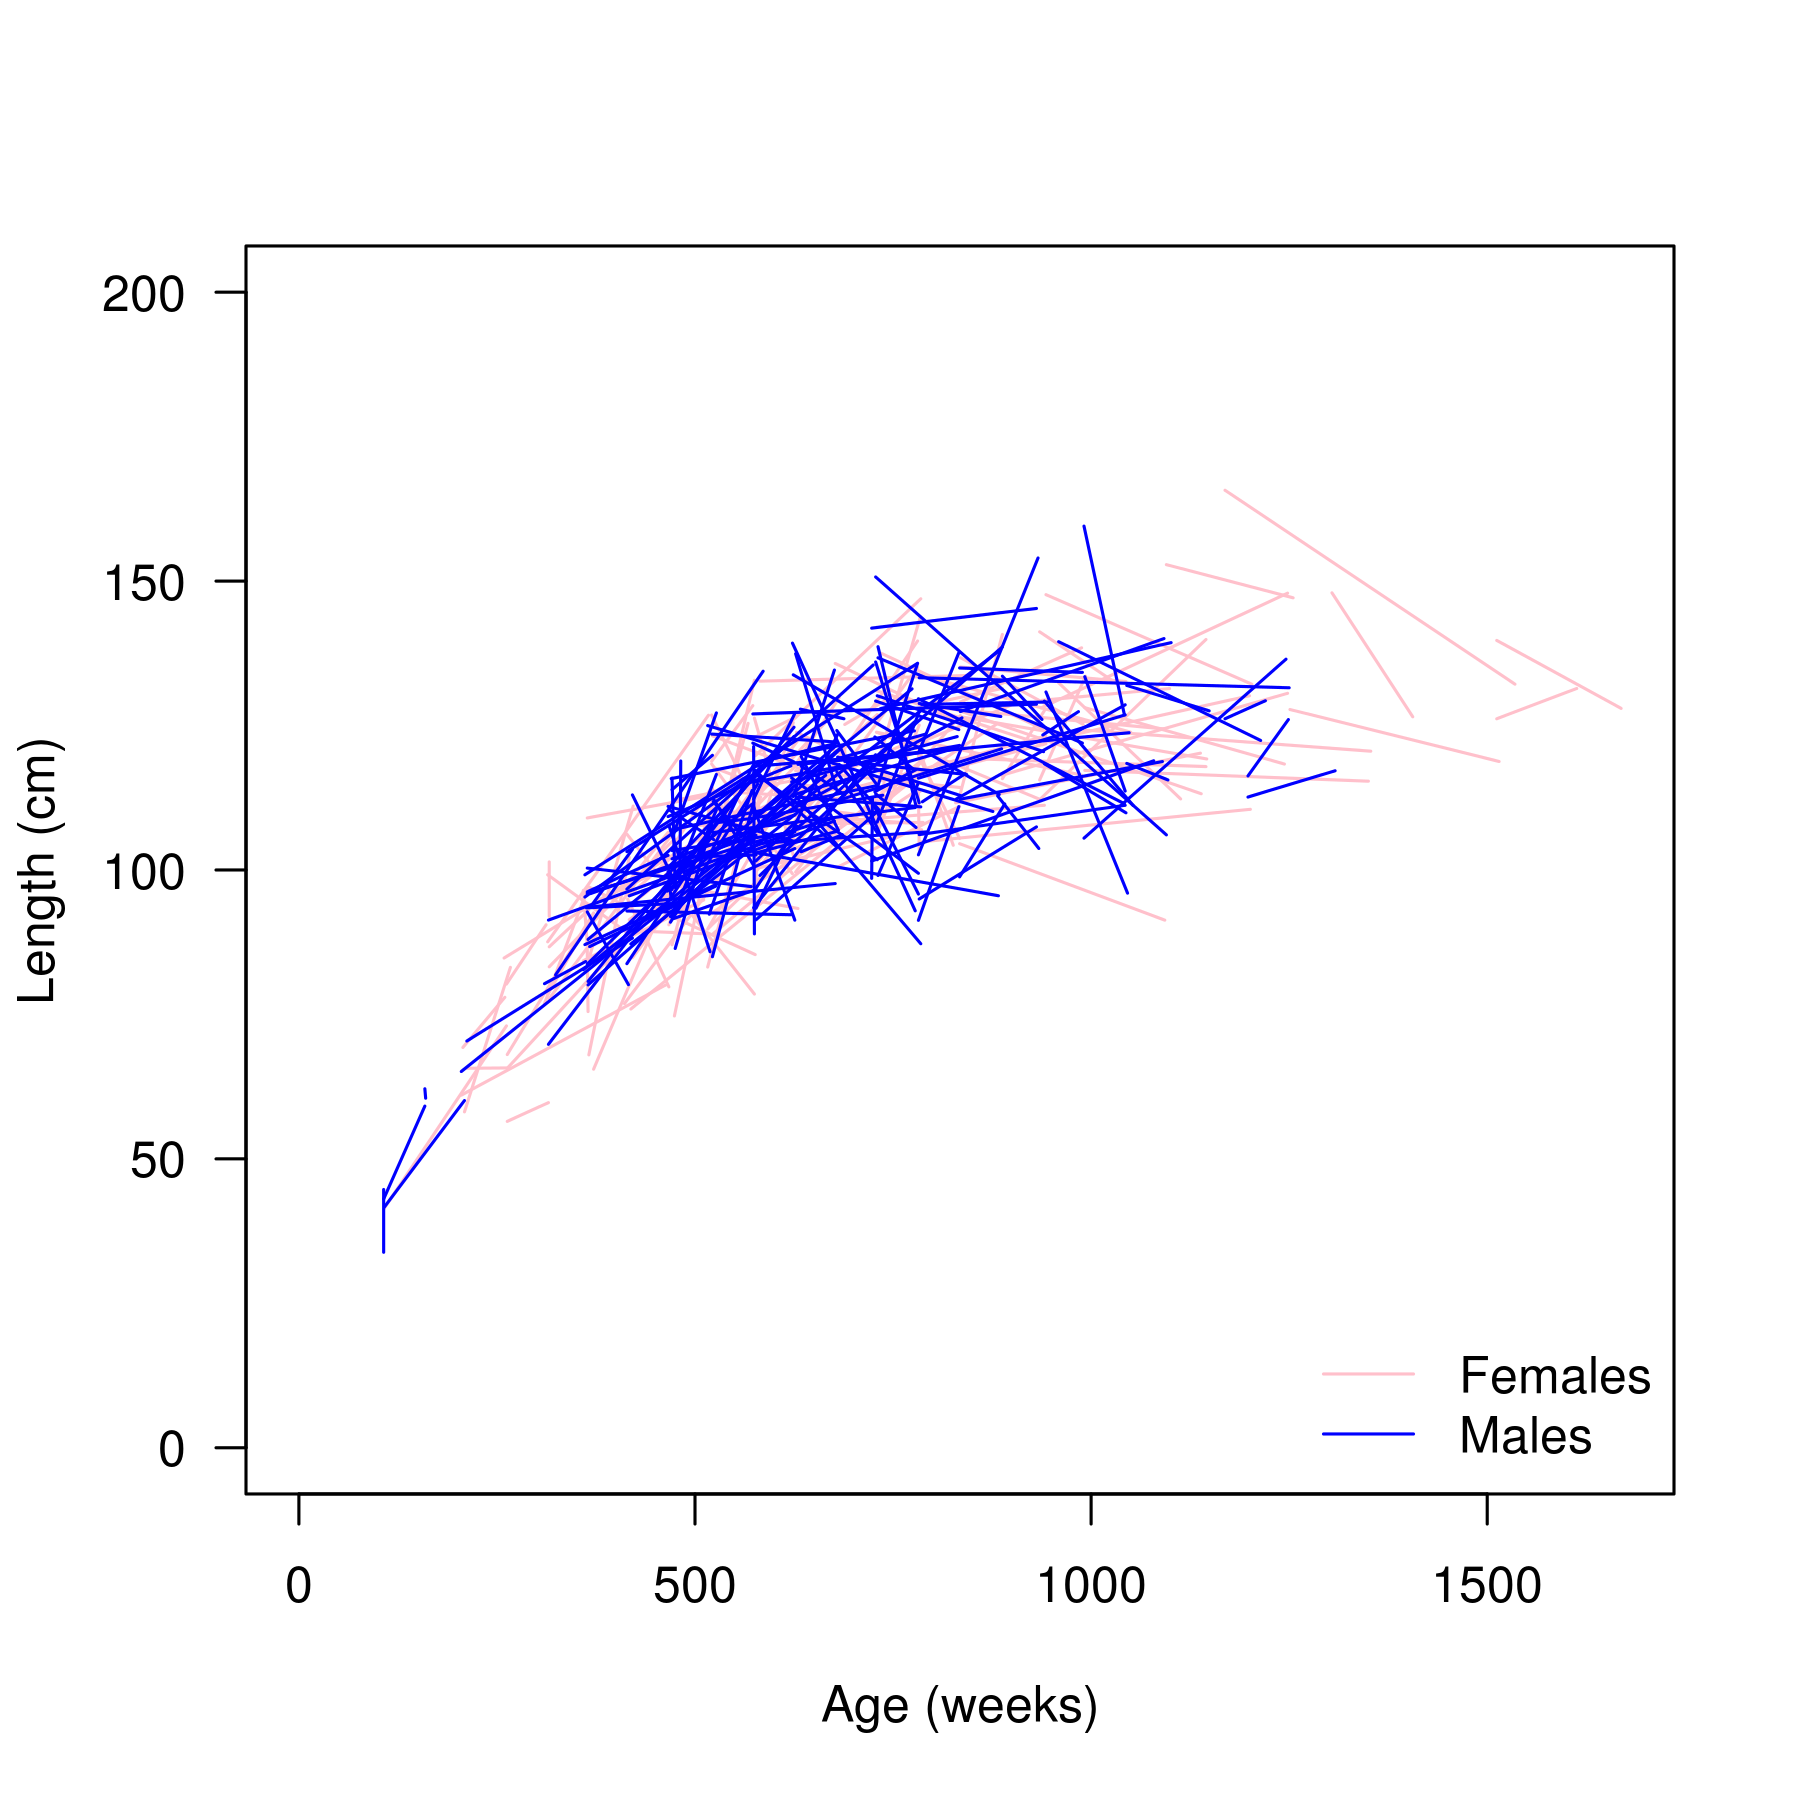
\includegraphics[width=0.49\linewidth]{../simulation/sims/growth-45.png}
  %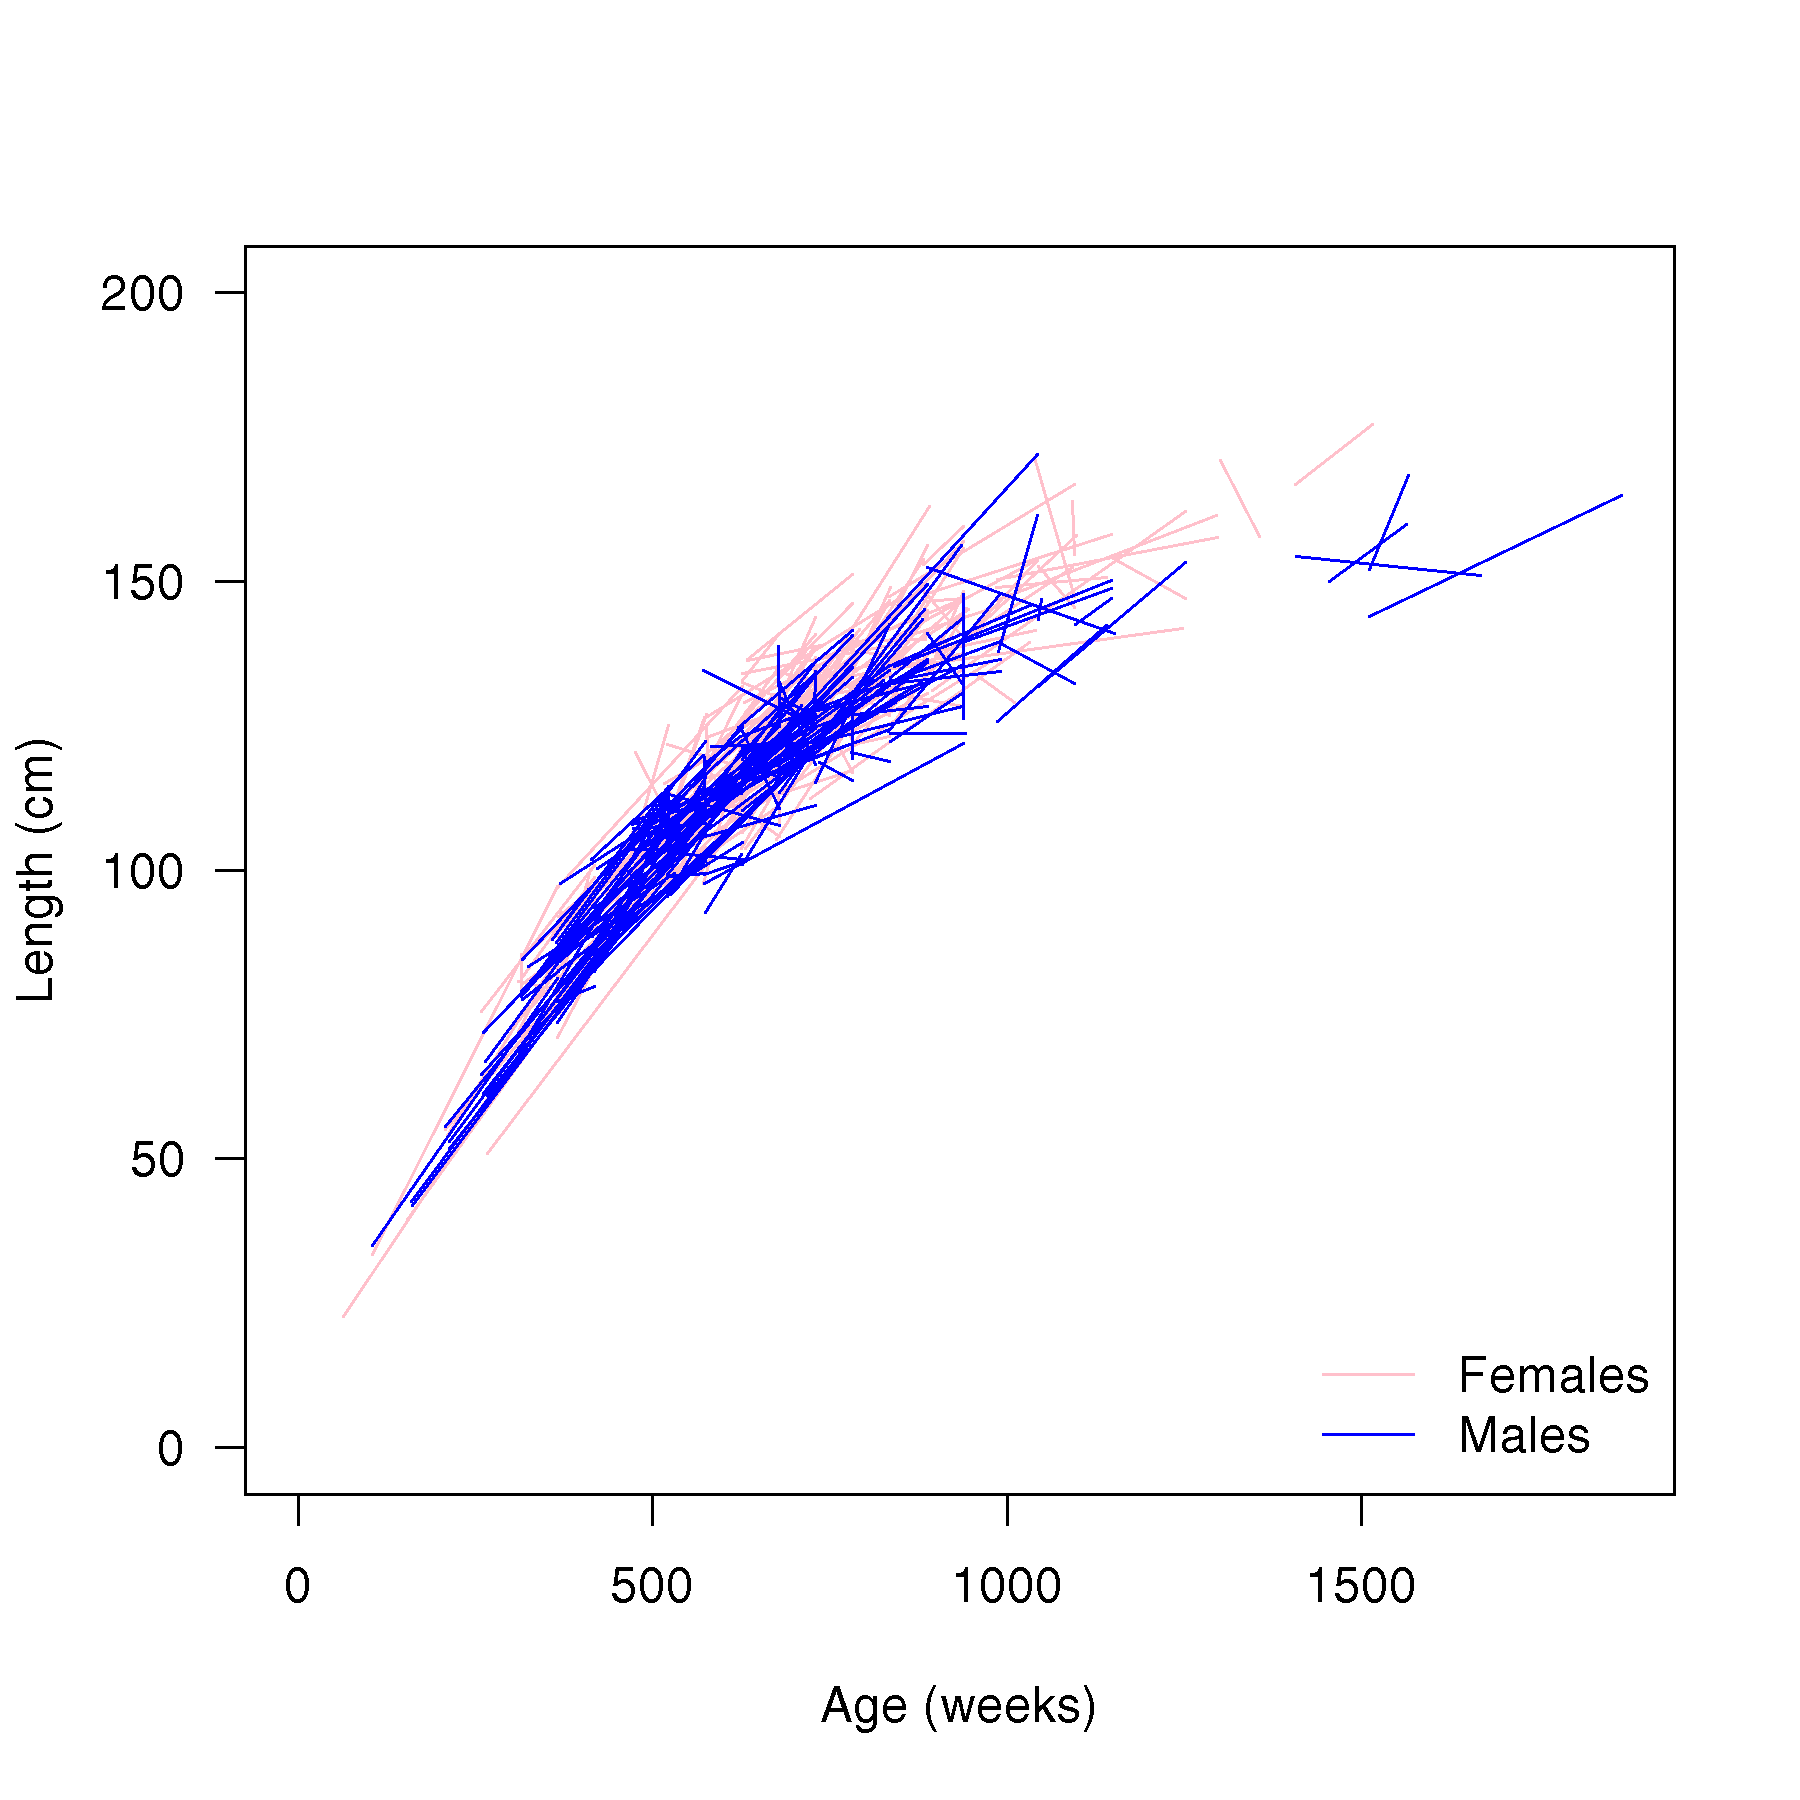
\includegraphics[width=0.49\linewidth]{../simulation/sims/growth-20.png}
  %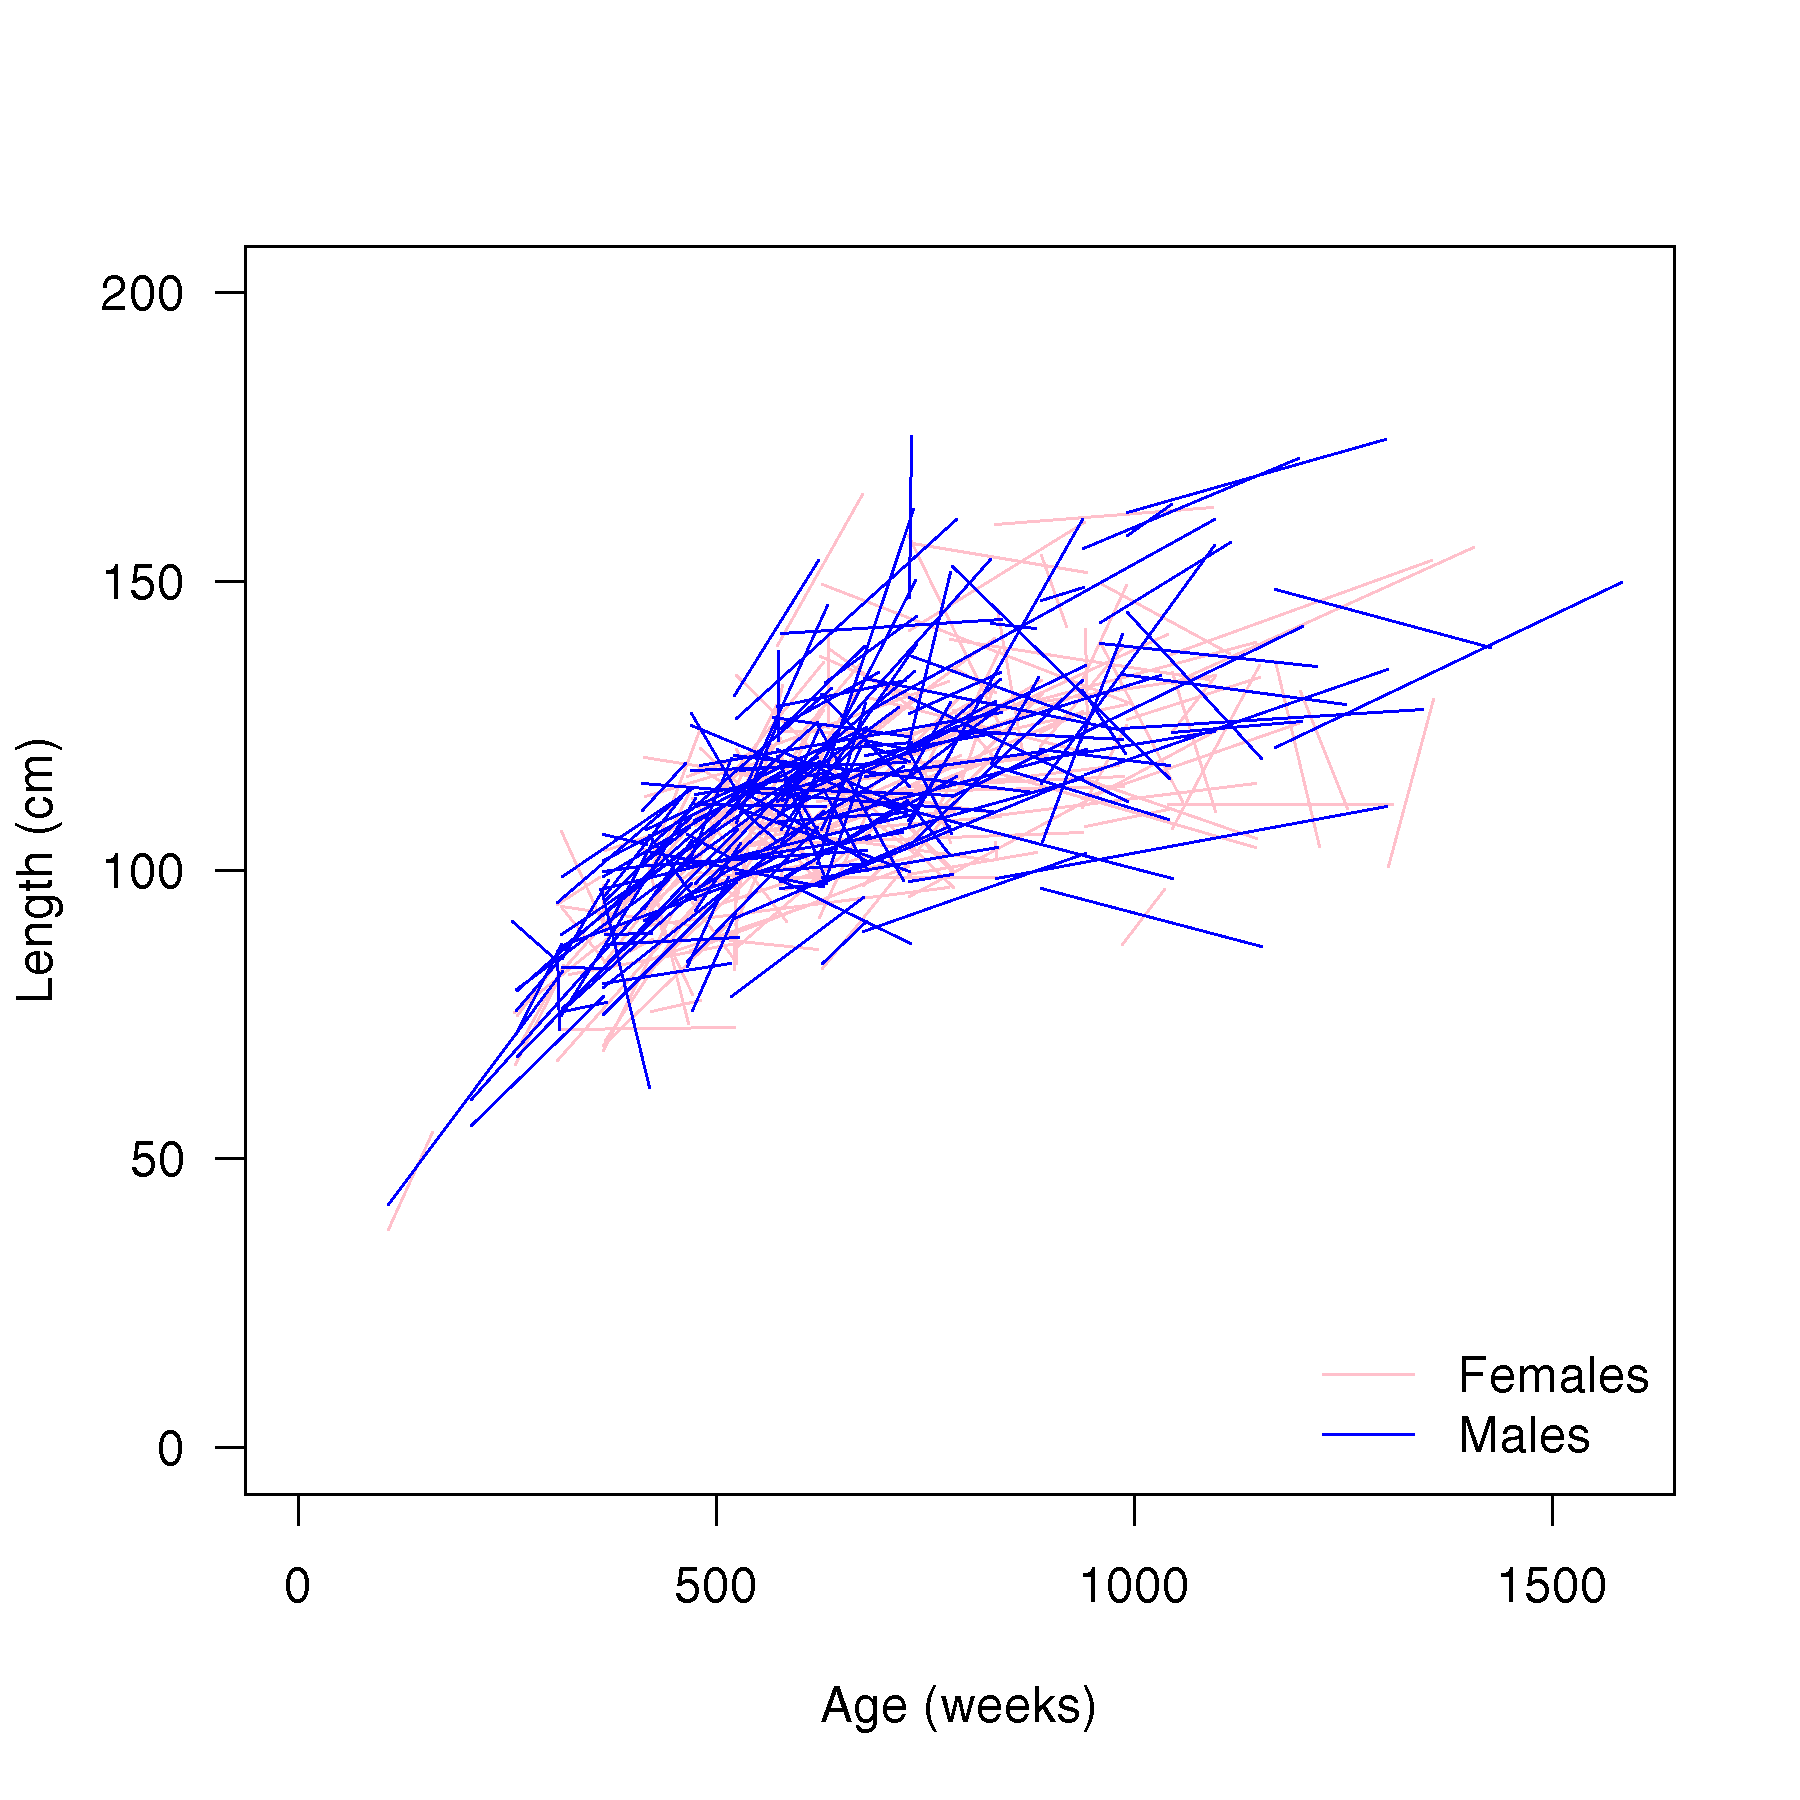
\includegraphics[width=0.49\linewidth]{../simulation/sims/growth-29.png}
  \begin{quote}
    \caption{Data sets for two models that were not pdH [top, simulations 1 and
      2], failed to converge [middle, simulations 6 and 45] and the only two
      datasets that were pdH [bottom, simulations 20 and 29].}
  \label{fig:1}
  \end{quote}
\end{figure}




\newpage\clearpage
%%%%%%%%%%%%%%%%%%%%%%%%%%%%%%%%%%%%%%%%%%%%%%%%%%%%%%%%%%%%%%%%%%%%%%%%%%%%%%%%%
\subsubsection{No random effects}
%%%%%%%%%%%%%%%%%%%%%%%%%%%%%%%%%%%%%%%%%%%%%%%%%%%%%%%%%%%%%%%%%%%%%%%%%%%%%%%%%
Here I tried turning of all random effects.
\begin{table}[!htbp]
  \begin{quote}
  \caption{\label{tab:} .} \small{
  \begin{center}
  \begin{tabular}{lrr}
  \hline
  Parameter      & Female & Male\\
  \hline
  $L_0$          & 0.0   & 6.9\\
  $\overline{b}$ & 0.003 & 0.003\\
  $\sigma_b$     & 0.0   & 0.0\\
  $\gamma$       & 0.4   & 0.4\\
  $\psi$         & 0.001 & 0.001\\
  $\sigma_o$     & 0.099 & 0.099\\
  $\sigma_z$     & 0.0   & 0.0\\
  $\sigma_y$     & 0.0   & 0.0\\
  \hline
  \end{tabular}
  \end{center}
  }
  \end{quote}
\end{table}

\begin{figure}[!htbp]
  \centering
  %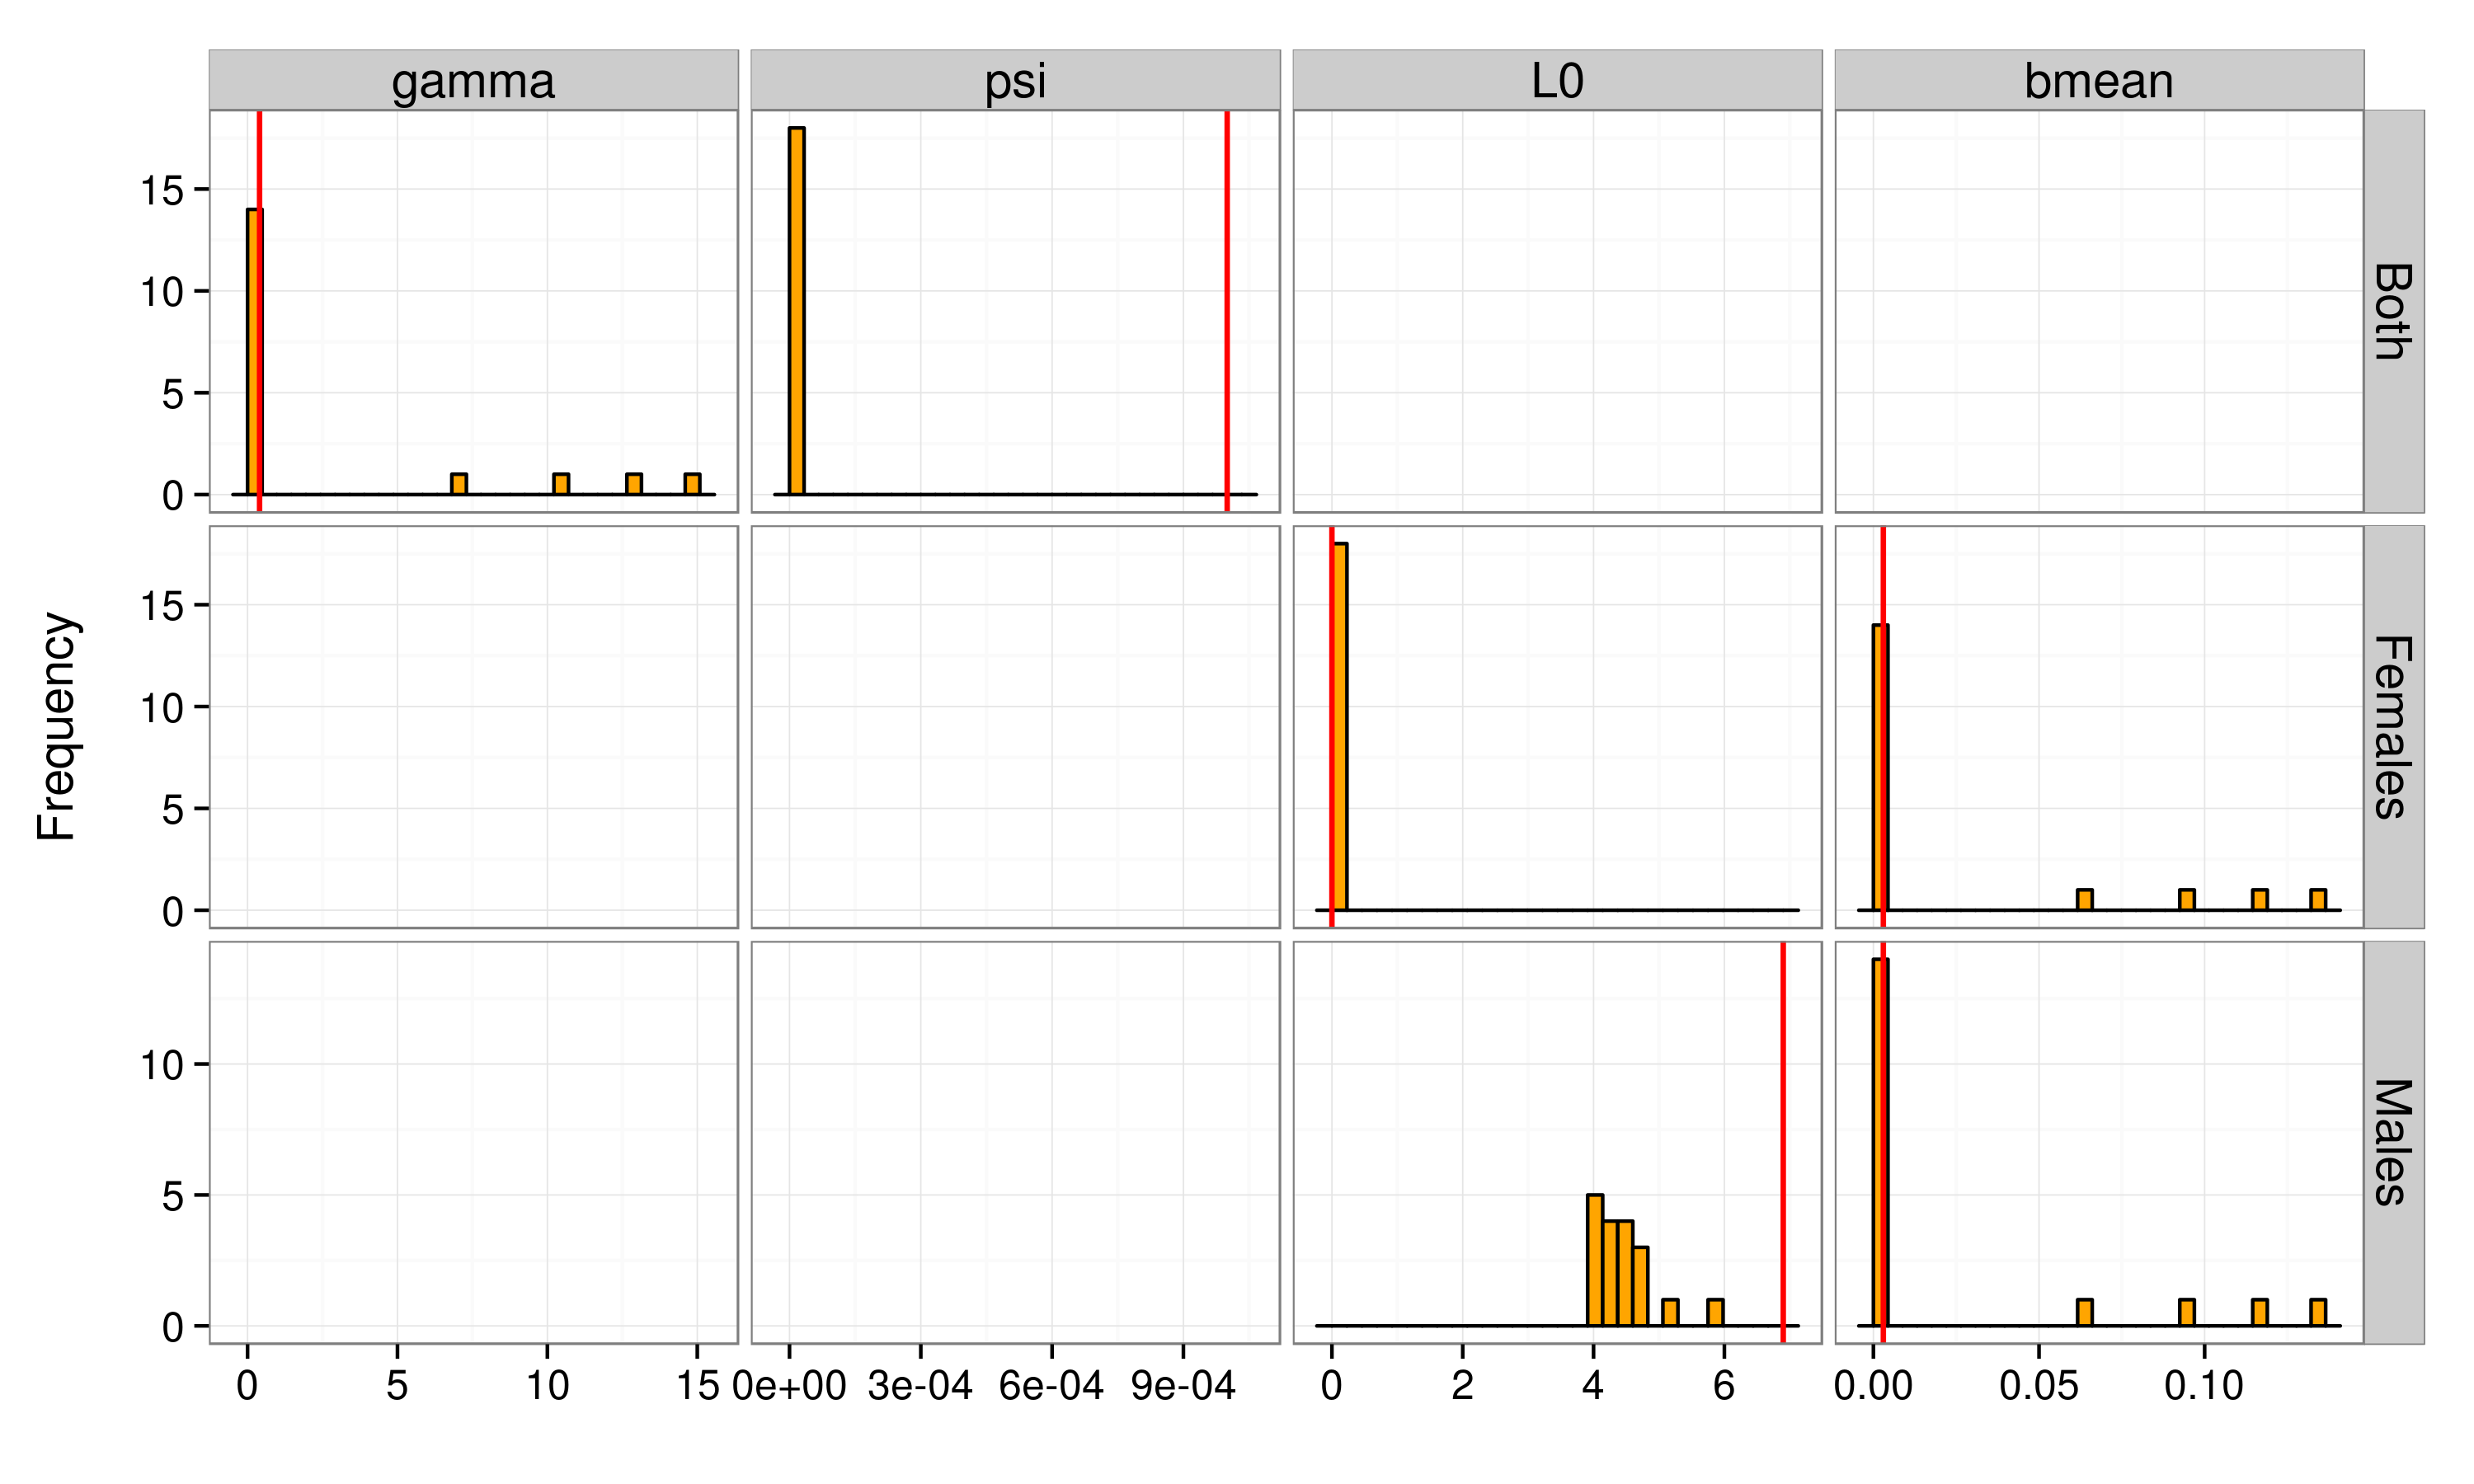
\includegraphics[width=\linewidth]{../simulation/sims/results/SimPars.png}
  %\includegraphics[width=\linewidth]{../simulation/sims/results/TracePars.png}
  \begin{quote}
    \caption{.}
  \label{fig:}
  \end{quote}
\end{figure}


%%%%%%%%%%%%%%%%%%%%%%%%%%%%%%%%%%%%%%%%%%%%%%%%%%%%%%%%%%%%%%%%%%%%%%%%%%%%%%%%%
\subsubsection{sims1}
%%%%%%%%%%%%%%%%%%%%%%%%%%%%%%%%%%%%%%%%%%%%%%%%%%%%%%%%%%%%%%%%%%%%%%%%%%%%%%%%%
This was our first attempt at estimating simulated data.  $L_0$ was simulated
as 43 and 50 for females and males respectively (Table~\ref{tab:sims1}).

$L_0$ was estimated without a prior penalty.  $b$ was treated as a random
effect.

80 of 100 fits were pdHess.  Looking at the histograms below there seems to be
two states that the model estimates are jumping between.  Looking at the trace
plots, when $\sigma_o$ is estimated high then the remaining parameters are
poorly estimated (Figure~\ref{fig:sims1}).

\begin{figure}[!htbp]
  \centering
  %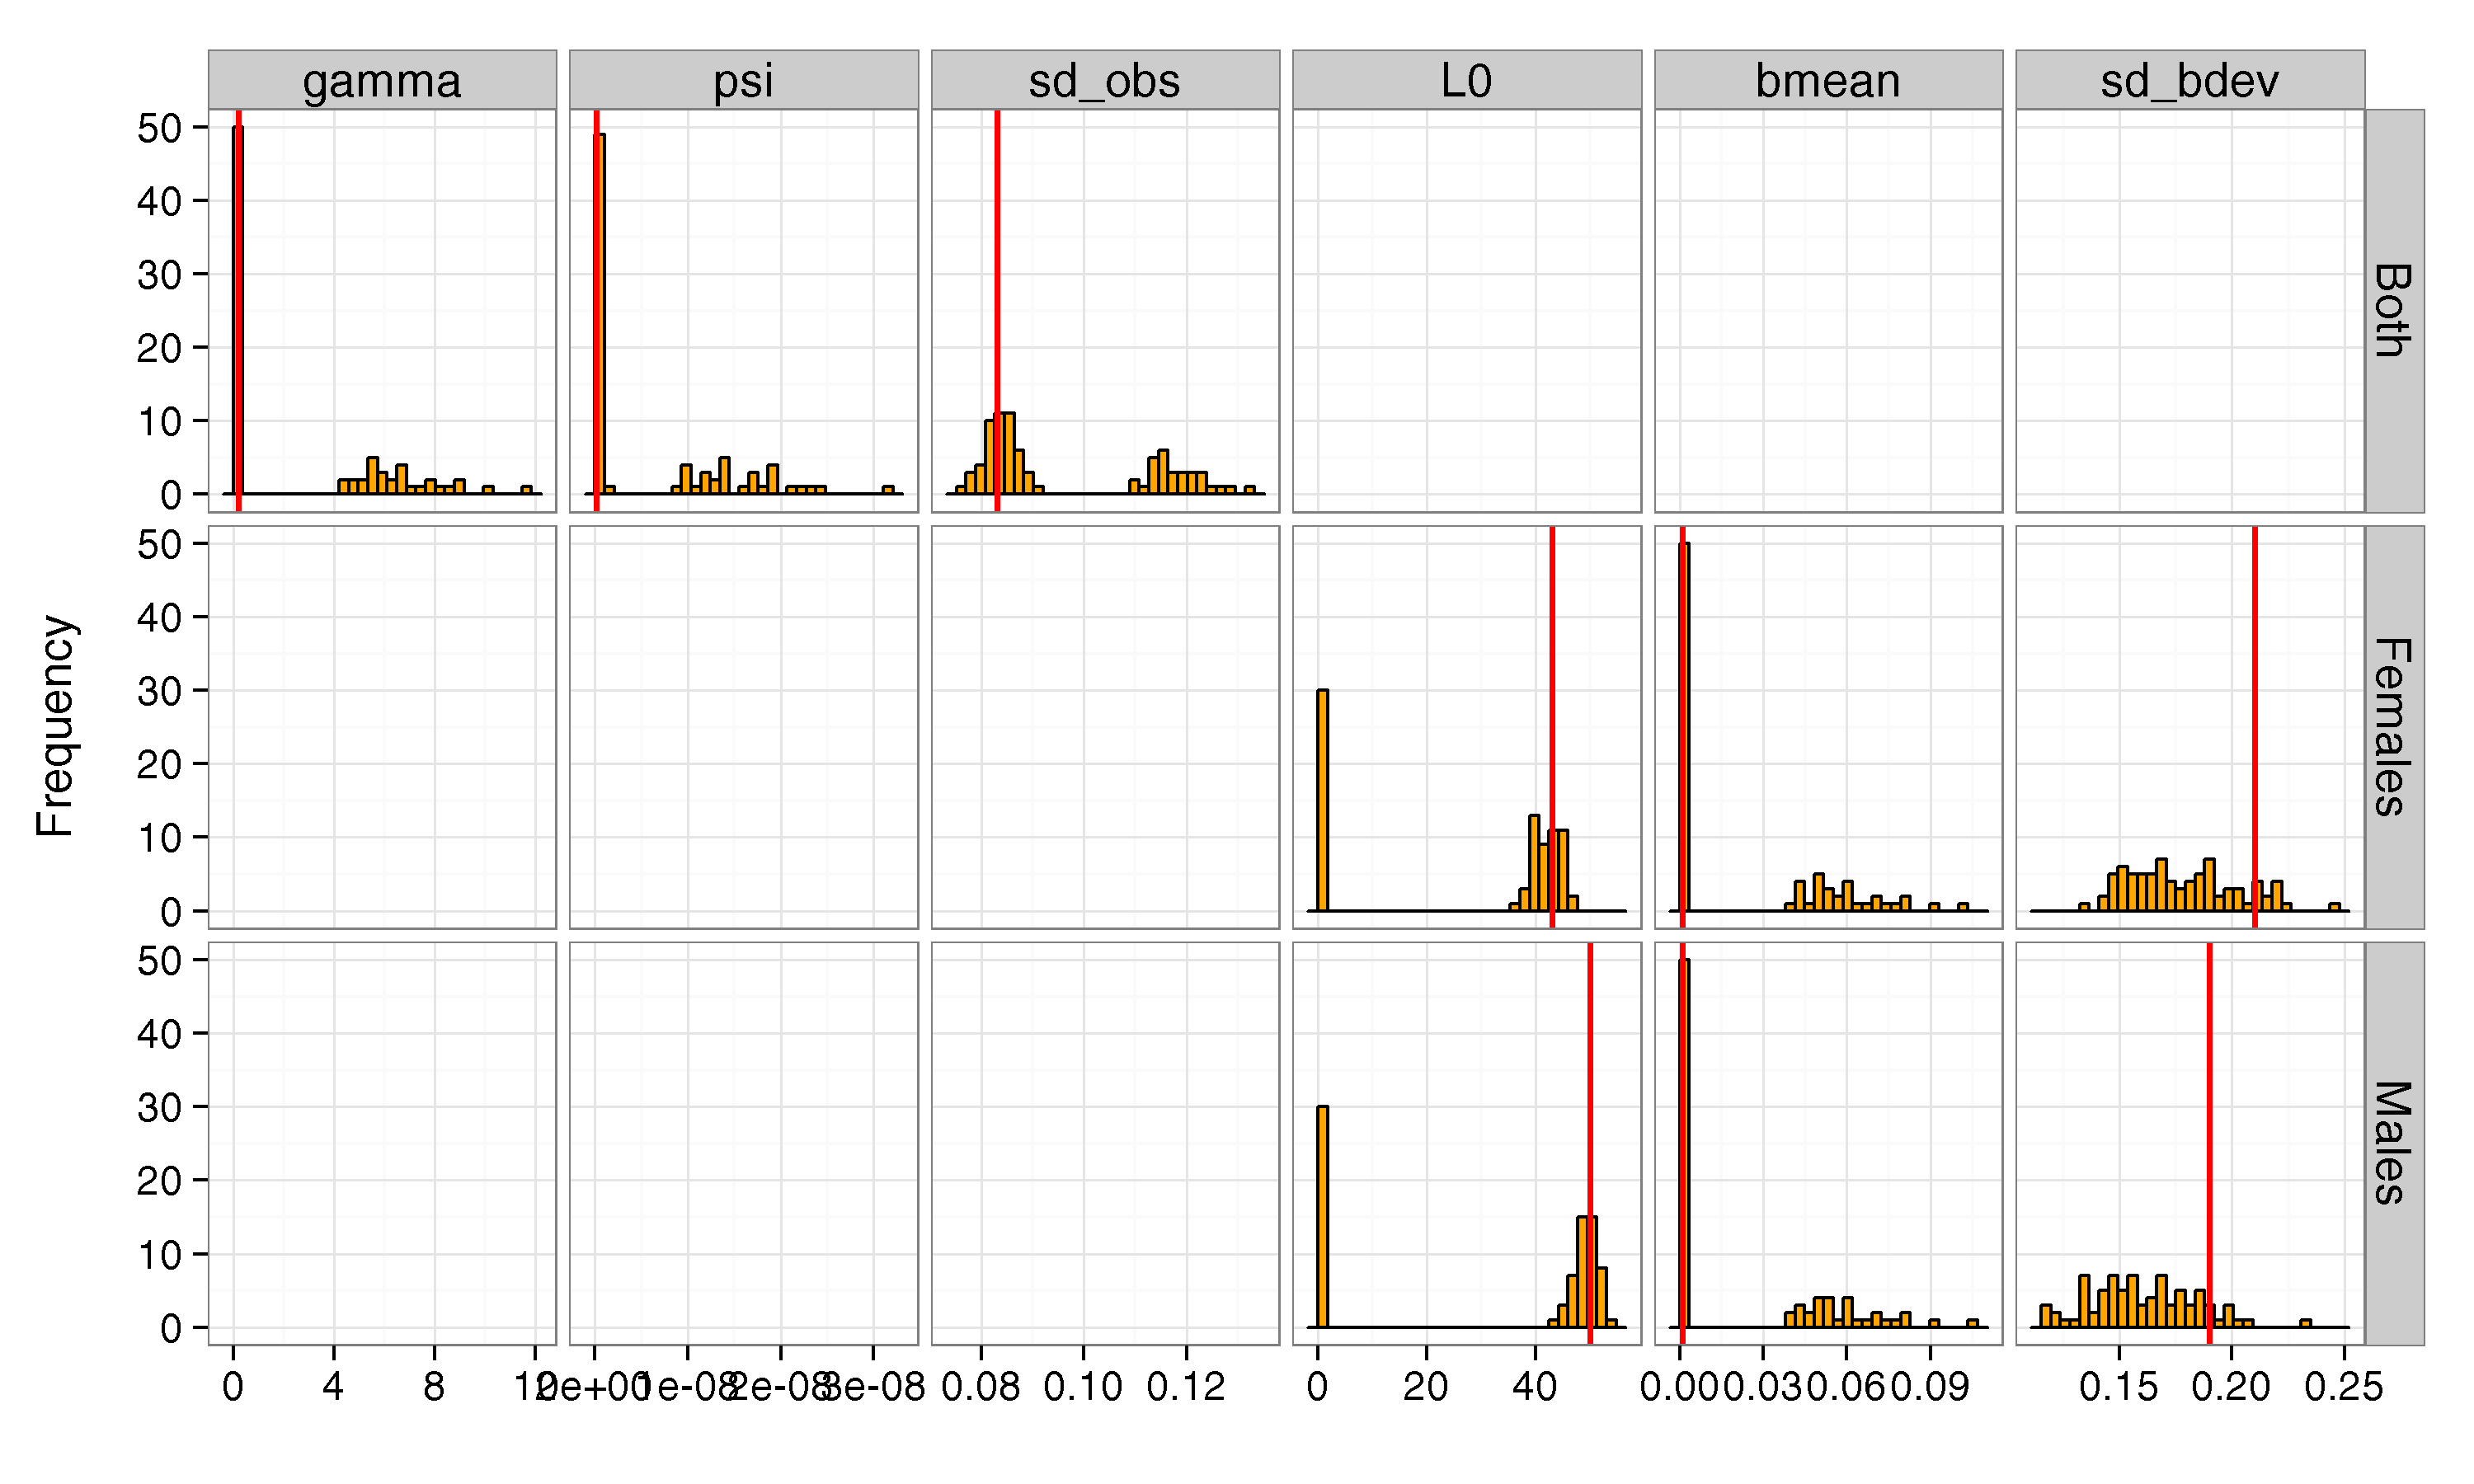
\includegraphics[width=\linewidth]{../simulation/sims1/results/SimPars.png}
  %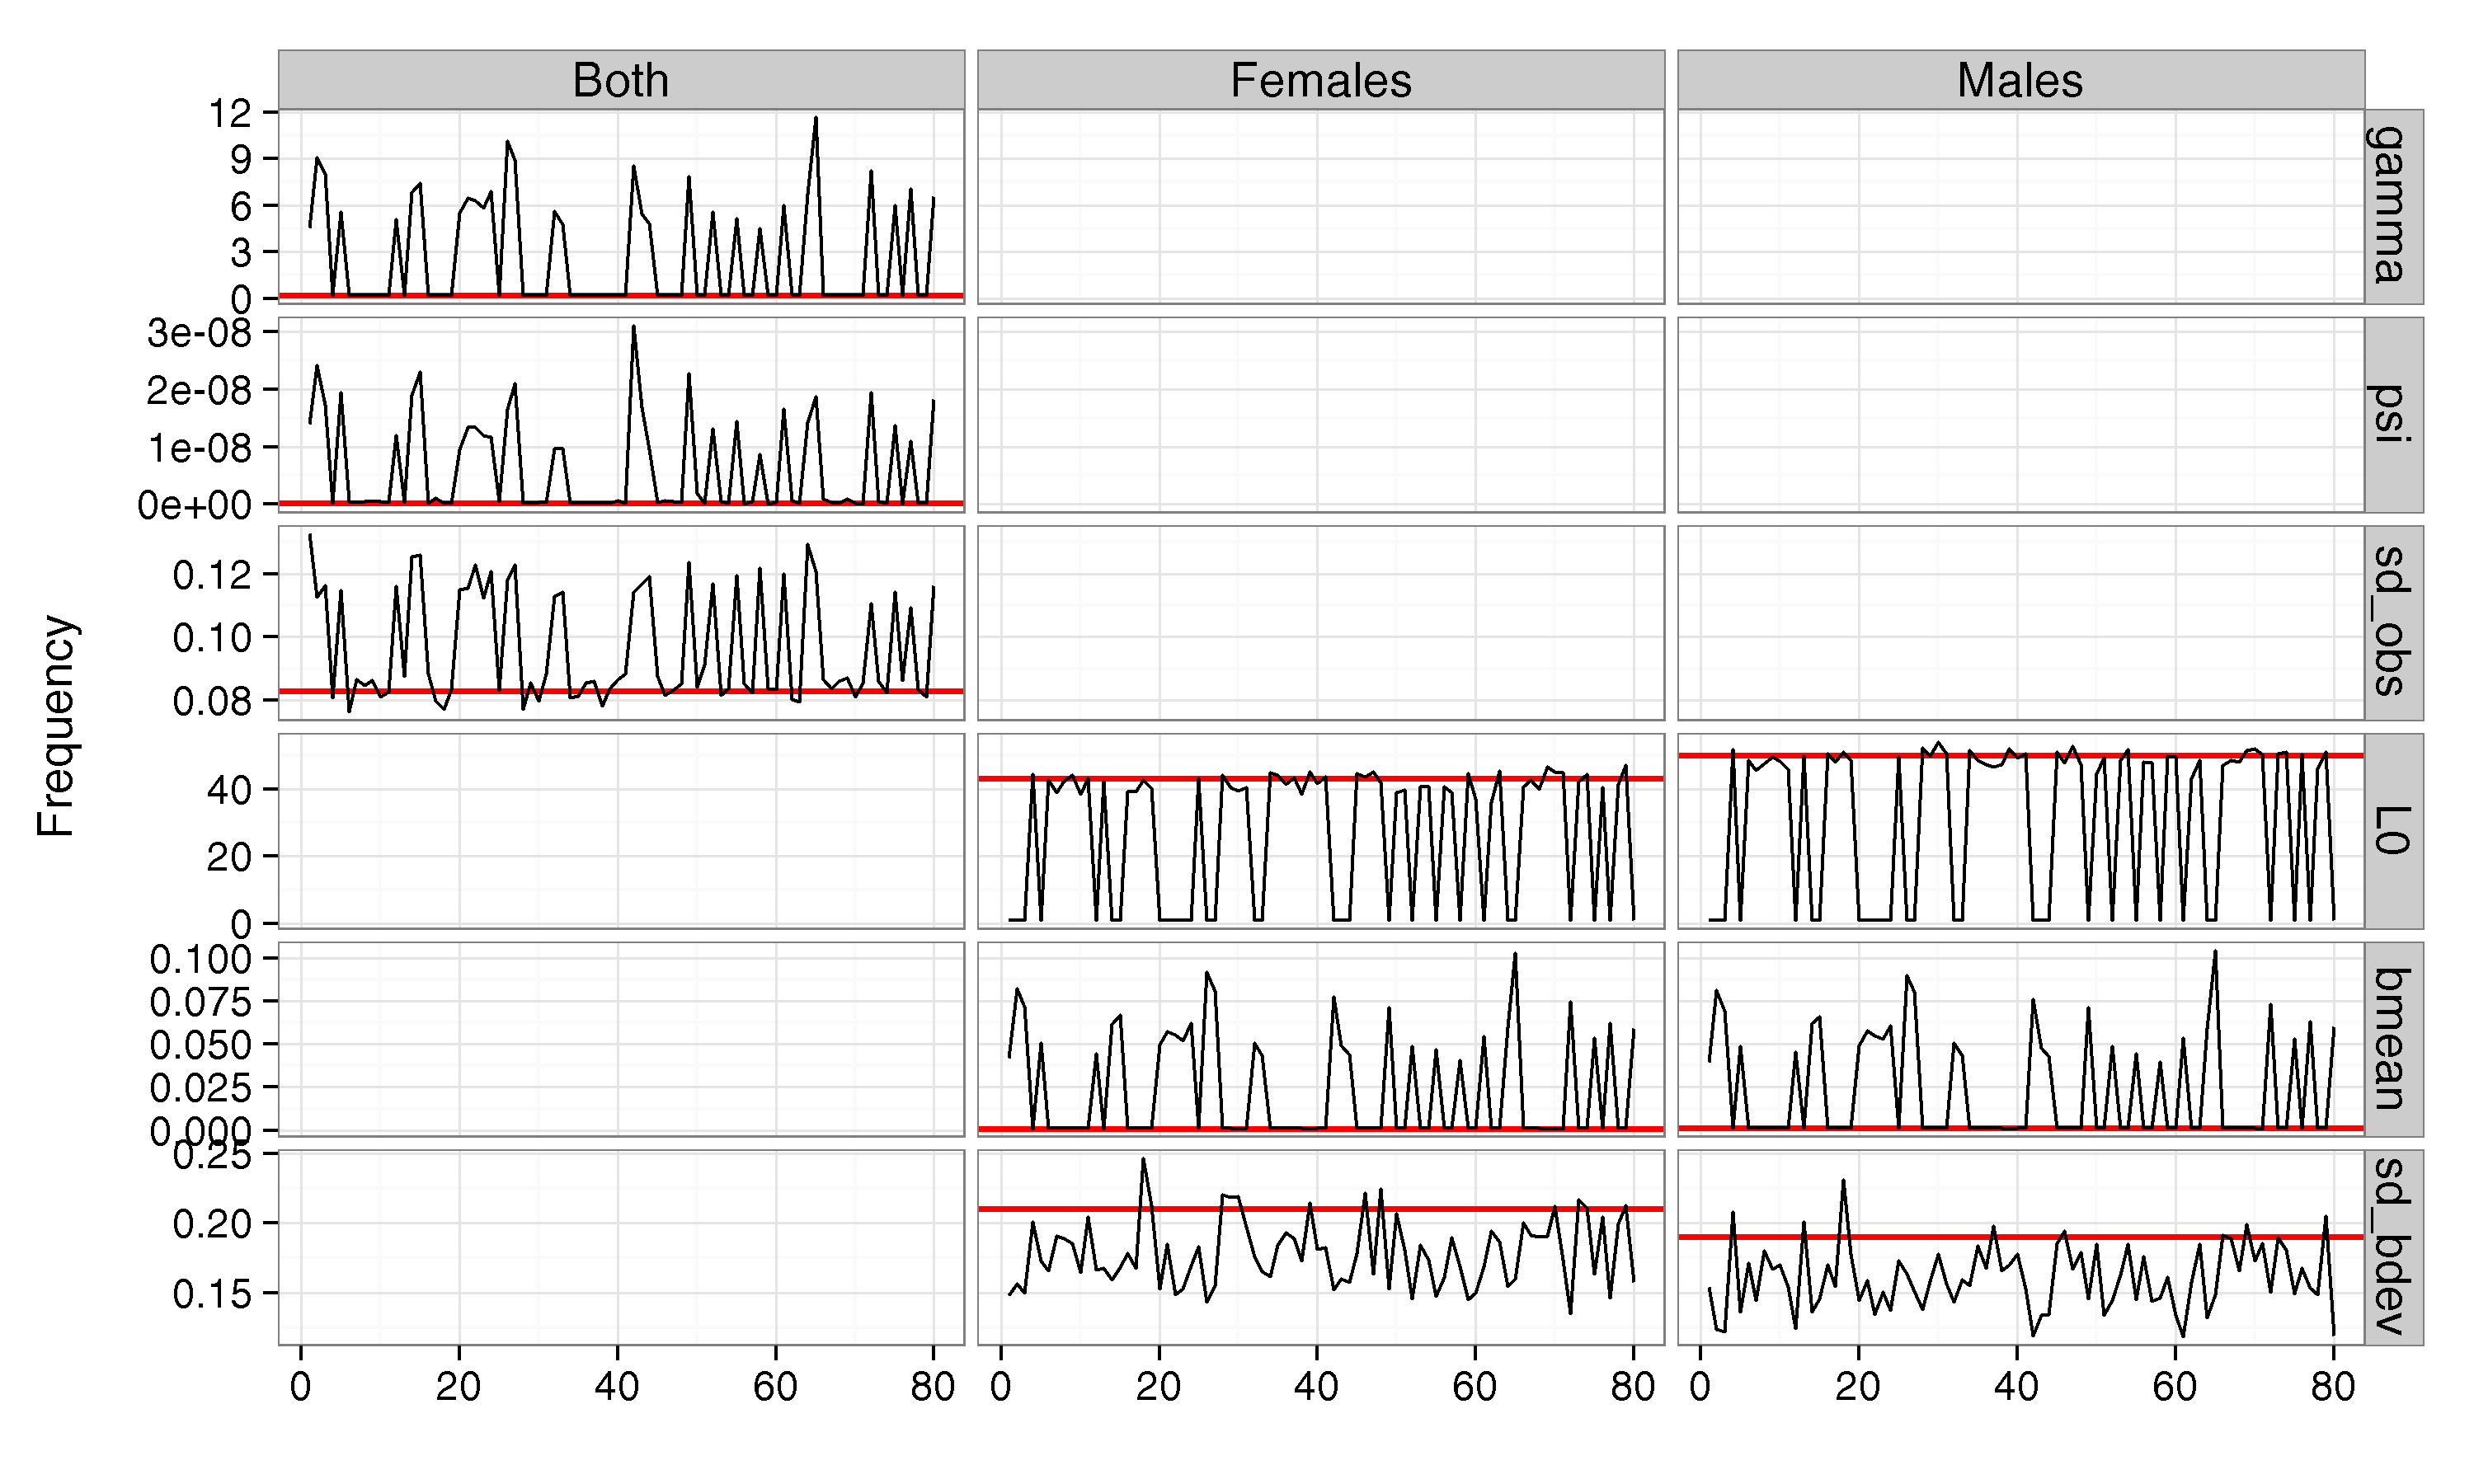
\includegraphics[width=\linewidth]{../simulation/sims1/results/TracePars.png}
  \begin{quote}
    \caption{pdH fits plotted only (80 of 100 fits were pdH)..}
    \label{fig:sims1}
  \end{quote}
\end{figure}


\newpage\clearpage
%%%%%%%%%%%%%%%%%%%%%%%%%%%%%%%%%%%%%%%%%%%%%%%%%%%%%%%%%%%%%%%%%%%%%%%%%%%%%%%%%
\subsubsection{sims2}
%%%%%%%%%%%%%%%%%%%%%%%%%%%%%%%%%%%%%%%%%%%%%%%%%%%%%%%%%%%%%%%%%%%%%%%%%%%%%%%%%
The simulation was run with $L_0$ values much closer to 0
(Table~\ref{tab:sims2}).

We placed a prior penalty on $L_0$ (a normal centered about 0).  Again, $b$ was
treated as a random effect.

57 of 100 fits were pdHess.  Doing a poor job of recovering $L_0$ for males.
Two states that seem to be linked to $\sigma_o$ again.  Not getting $\psi$ at
all (Figure~\ref{fig:sims2}).
\begin{table}[!htbp]
  \begin{quote}
    \caption{\label{tab:sims2} .} \small{
      \begin{center}
        \begin{tabular}{lrr}
          \hline
          Parameter      & Female & Male\\
          \hline
          $L_0$          & 0.0   & 6.9\\
          $\overline{b}$ & 0.003 & 0.003\\
          $\sigma_b$     & 0.106 & 0.112\\
          $\gamma$       & 0.4   & 0.4\\
          $\psi$         & 0.001 & 0.001\\
          $\sigma_o$     & 0.099 & 0.099\\
          $\sigma_z$     & 0.0   & 0.0\\
          $\sigma_y$     & 0.0   & 0.0\\
          \hline
        \end{tabular}
      \end{center}
    }
  \end{quote}
\end{table}

\begin{figure}[!htbp]
  \centering
  %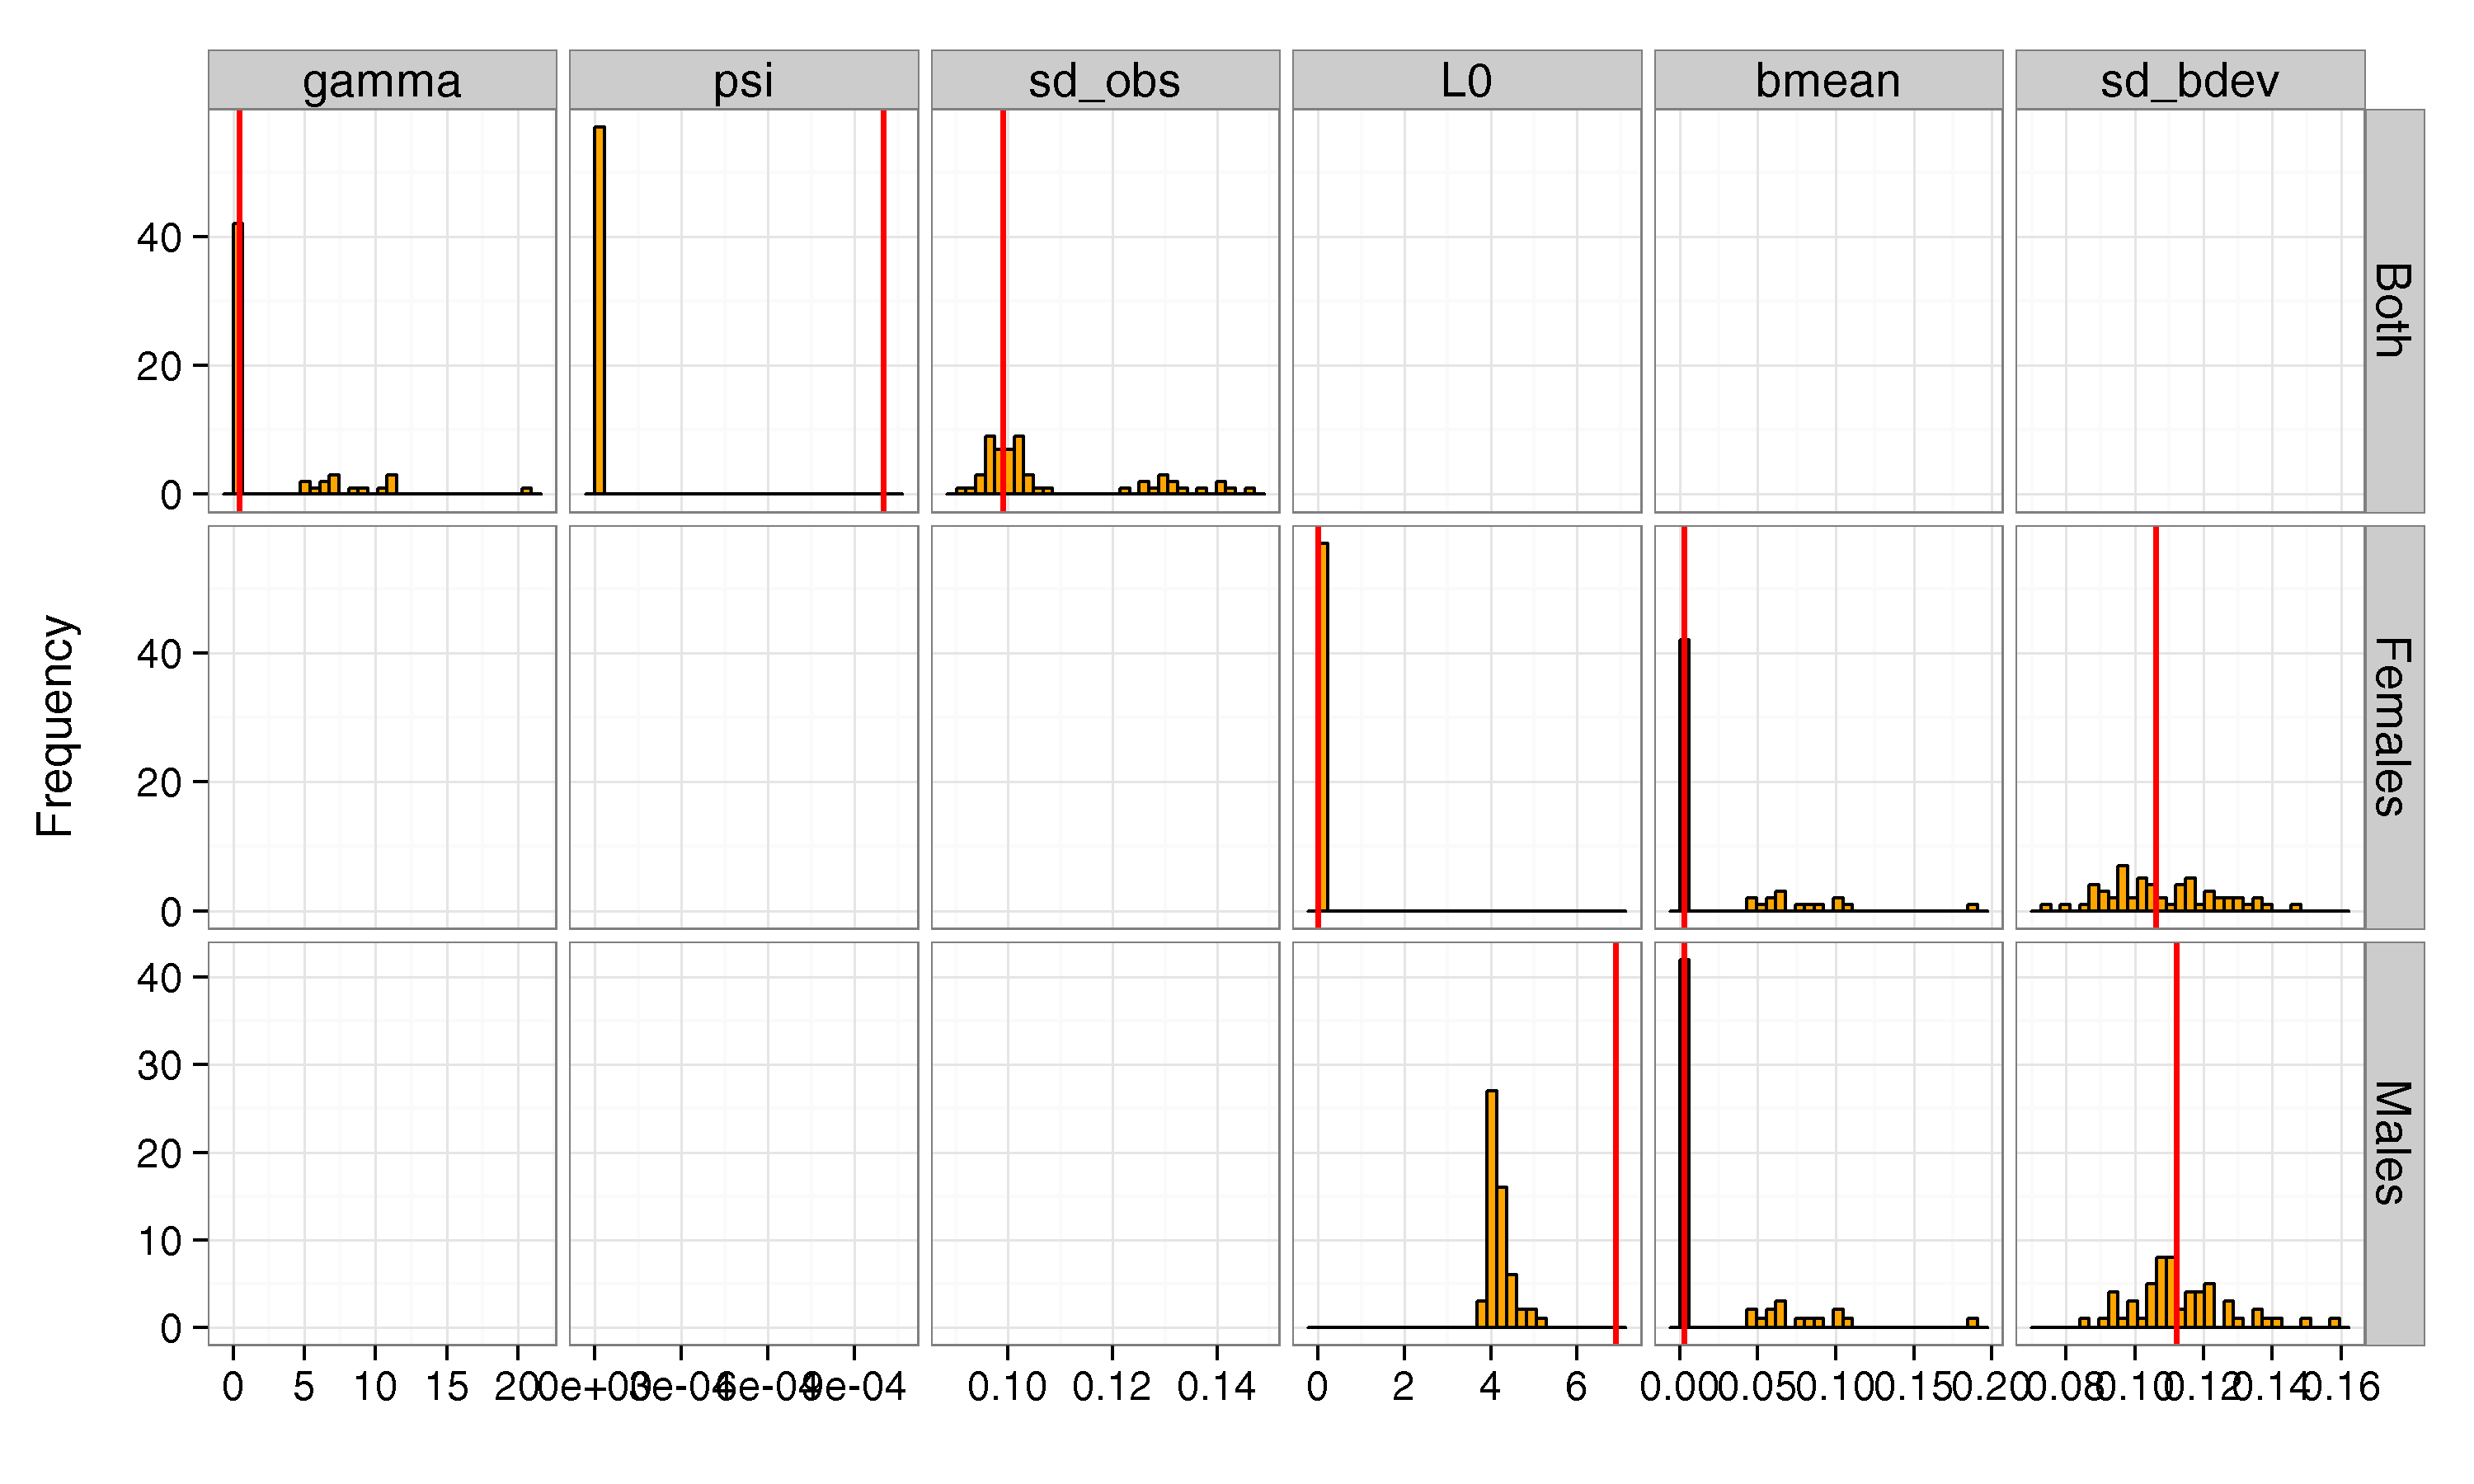
\includegraphics[width=\linewidth]{../simulation/sims2/results/SimPars.png}
  %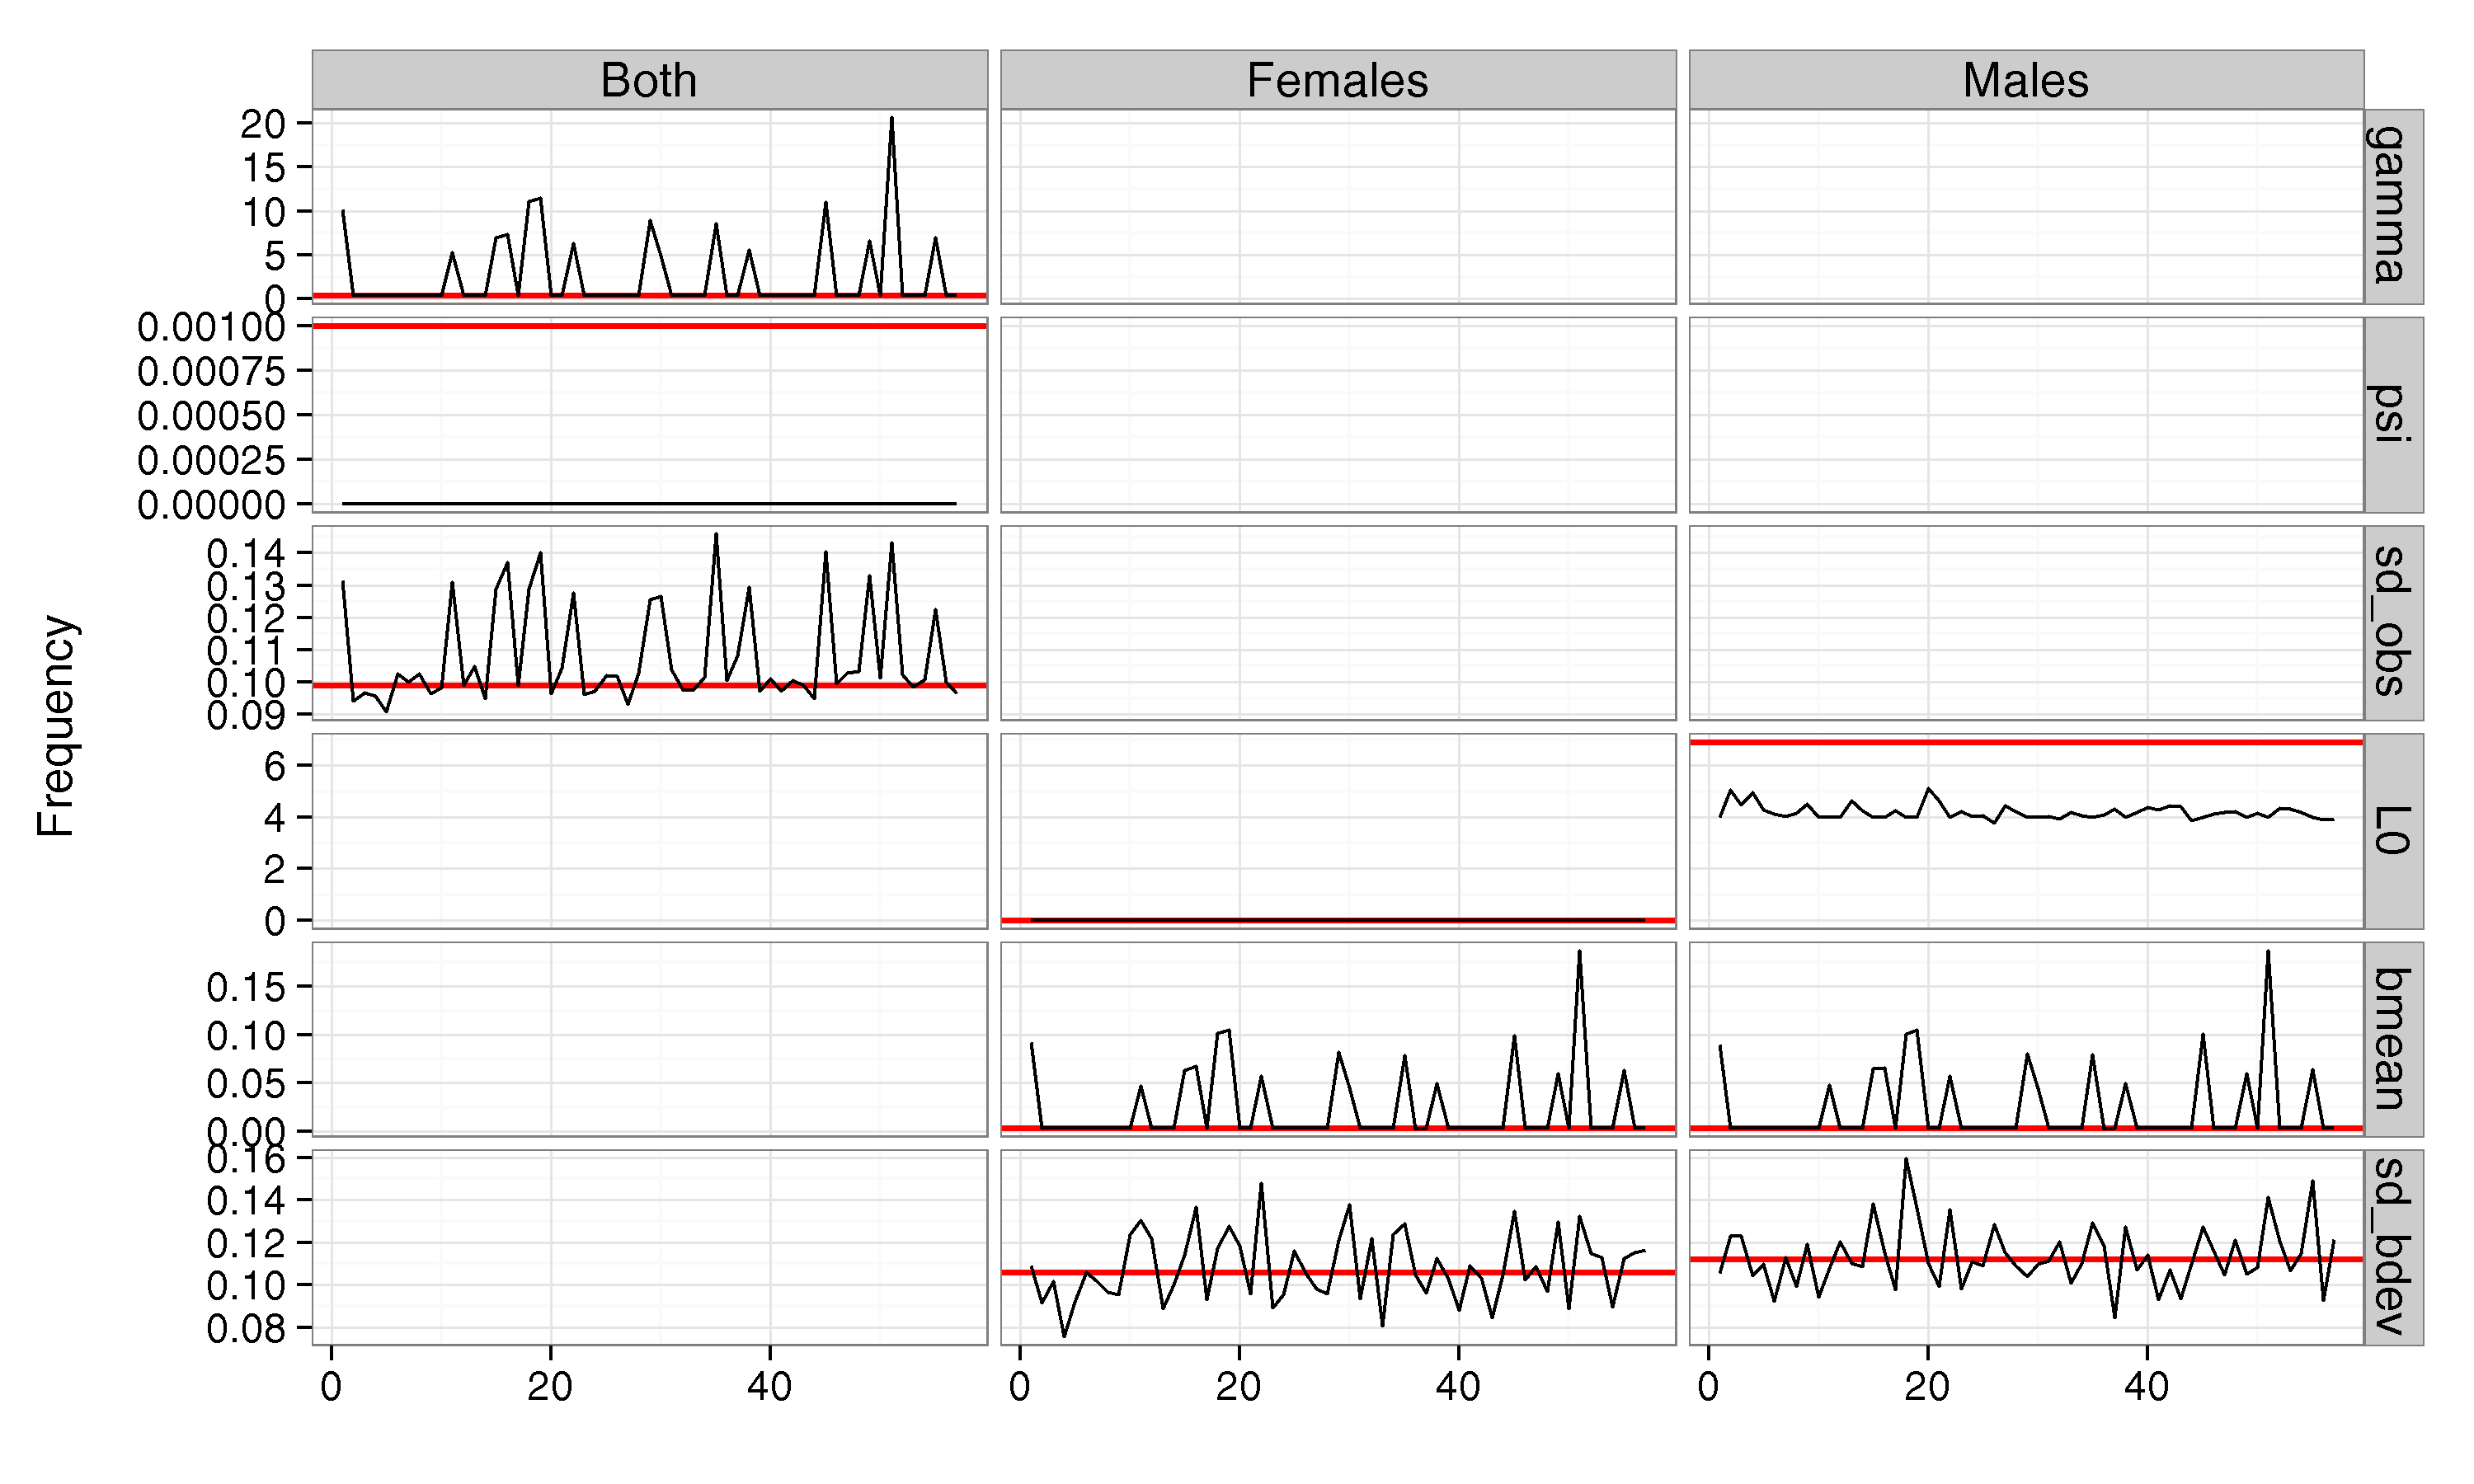
\includegraphics[width=\linewidth]{../simulation/sims2/results/TracePars.png}
  \begin{quote}
    \caption{pdH fits plotted only (57 of 100 fits were pdH).}
    \label{fig:sims2}
  \end{quote}
\end{figure}

\begin{figure}[!htbp]
  \centering
  %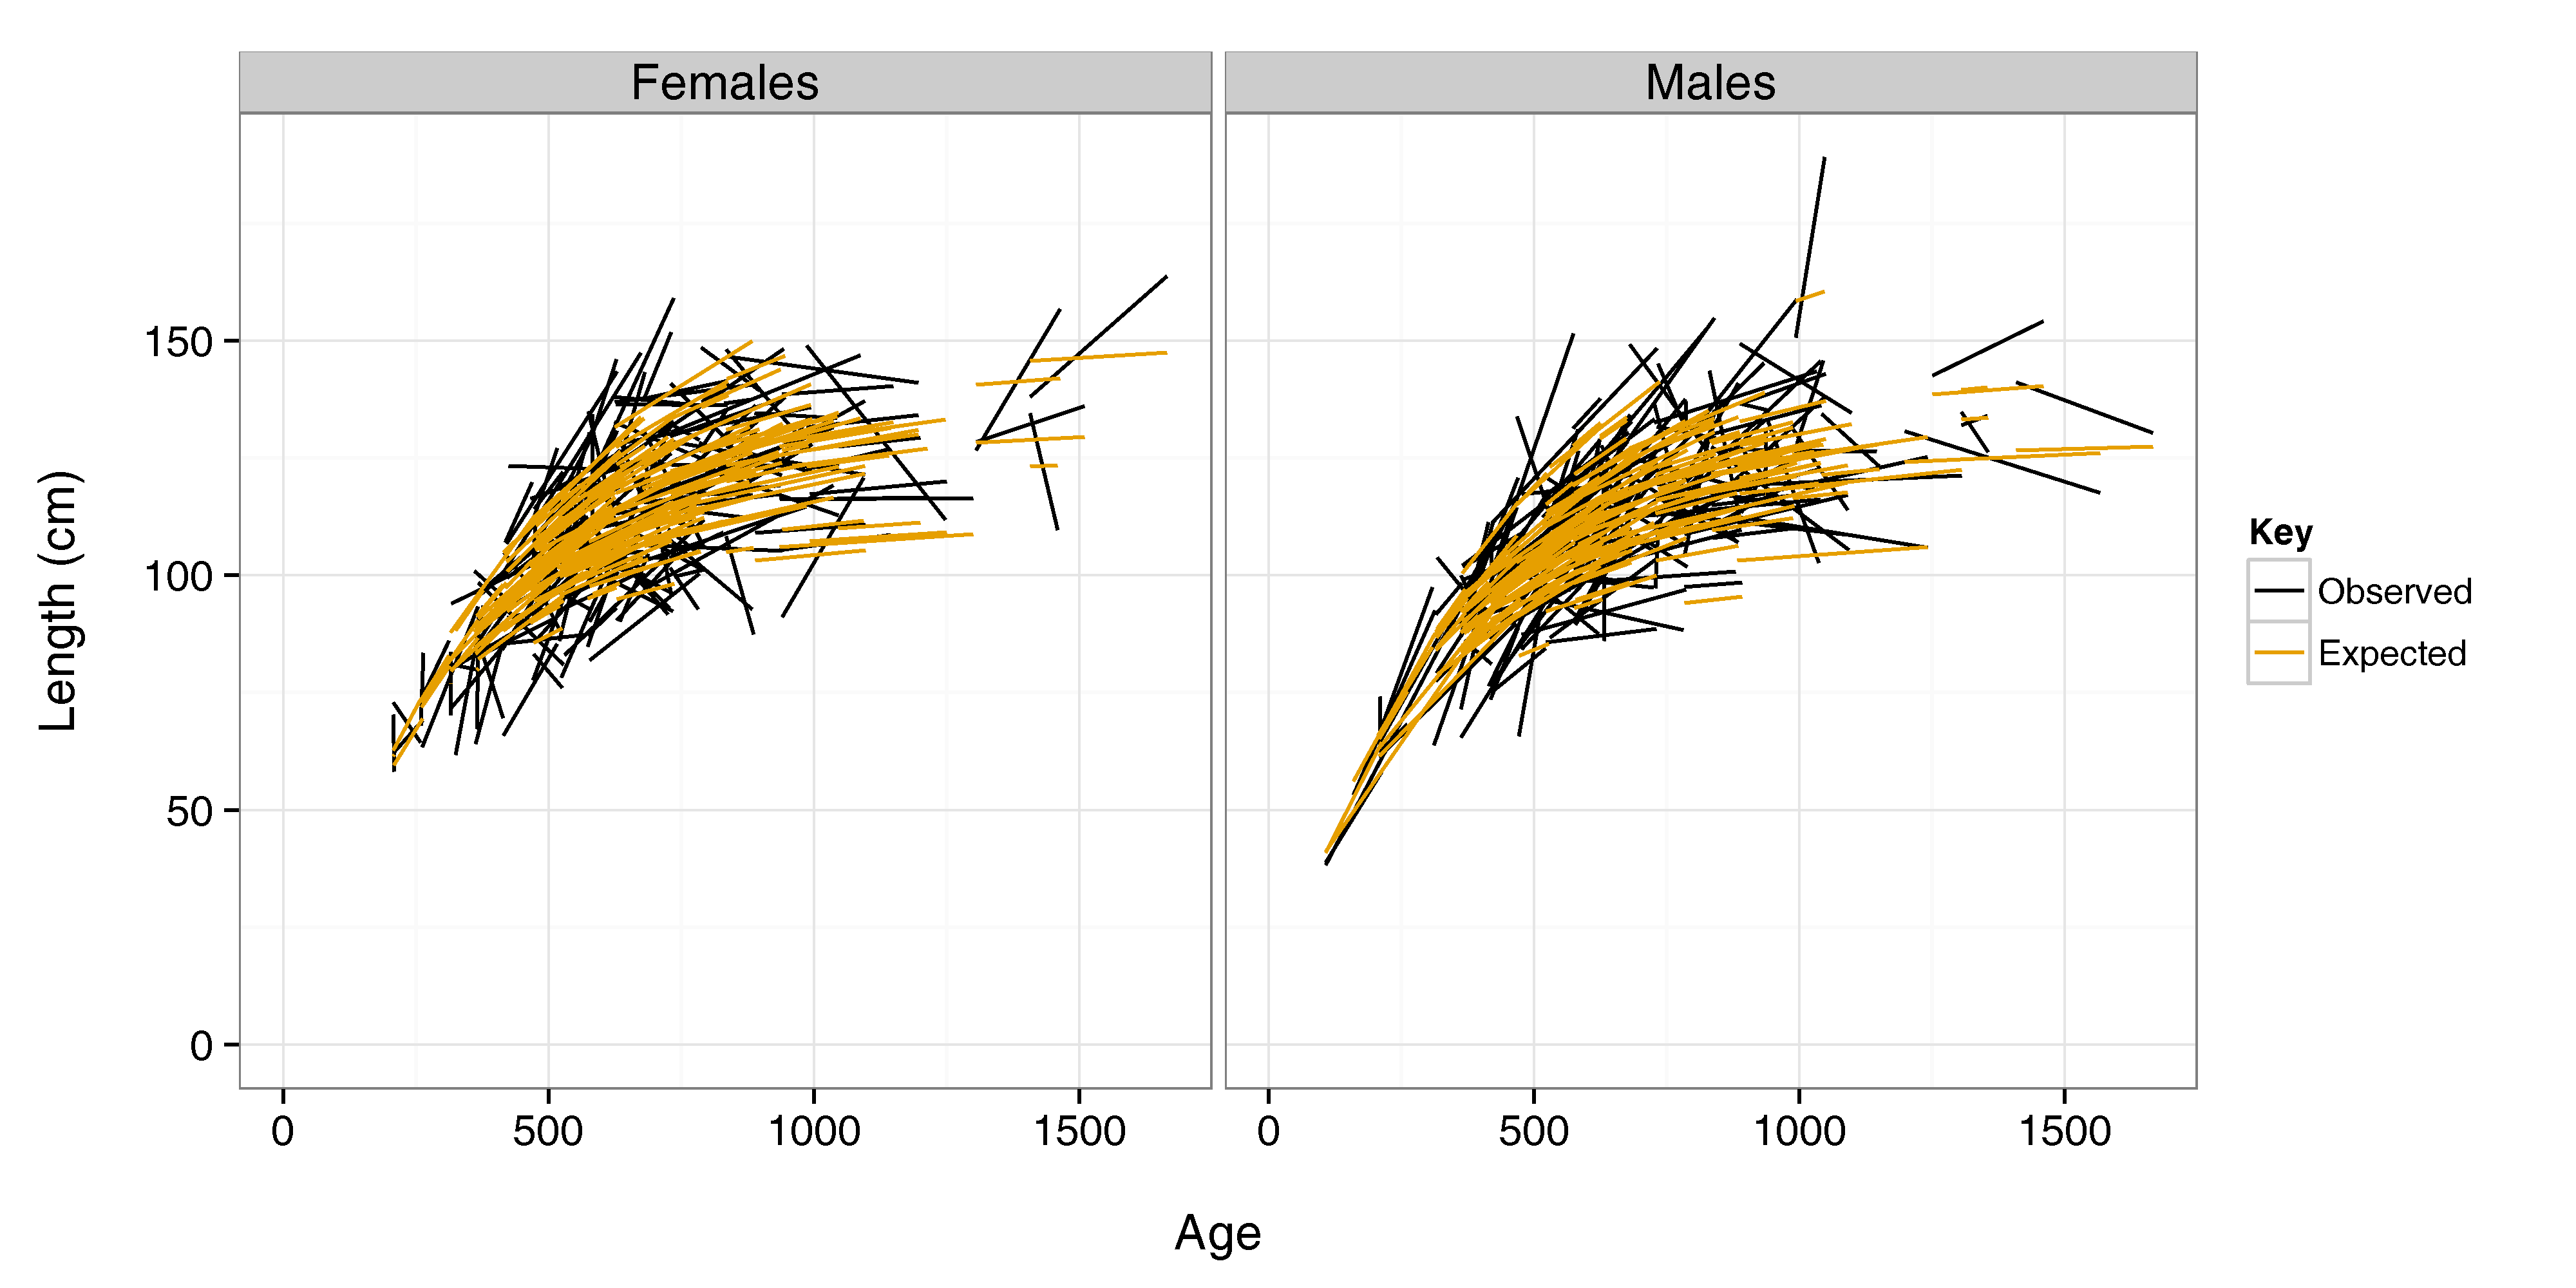
\includegraphics[width=\linewidth]{../simulation/sims2/results/IndivGrowth_3.png}
  %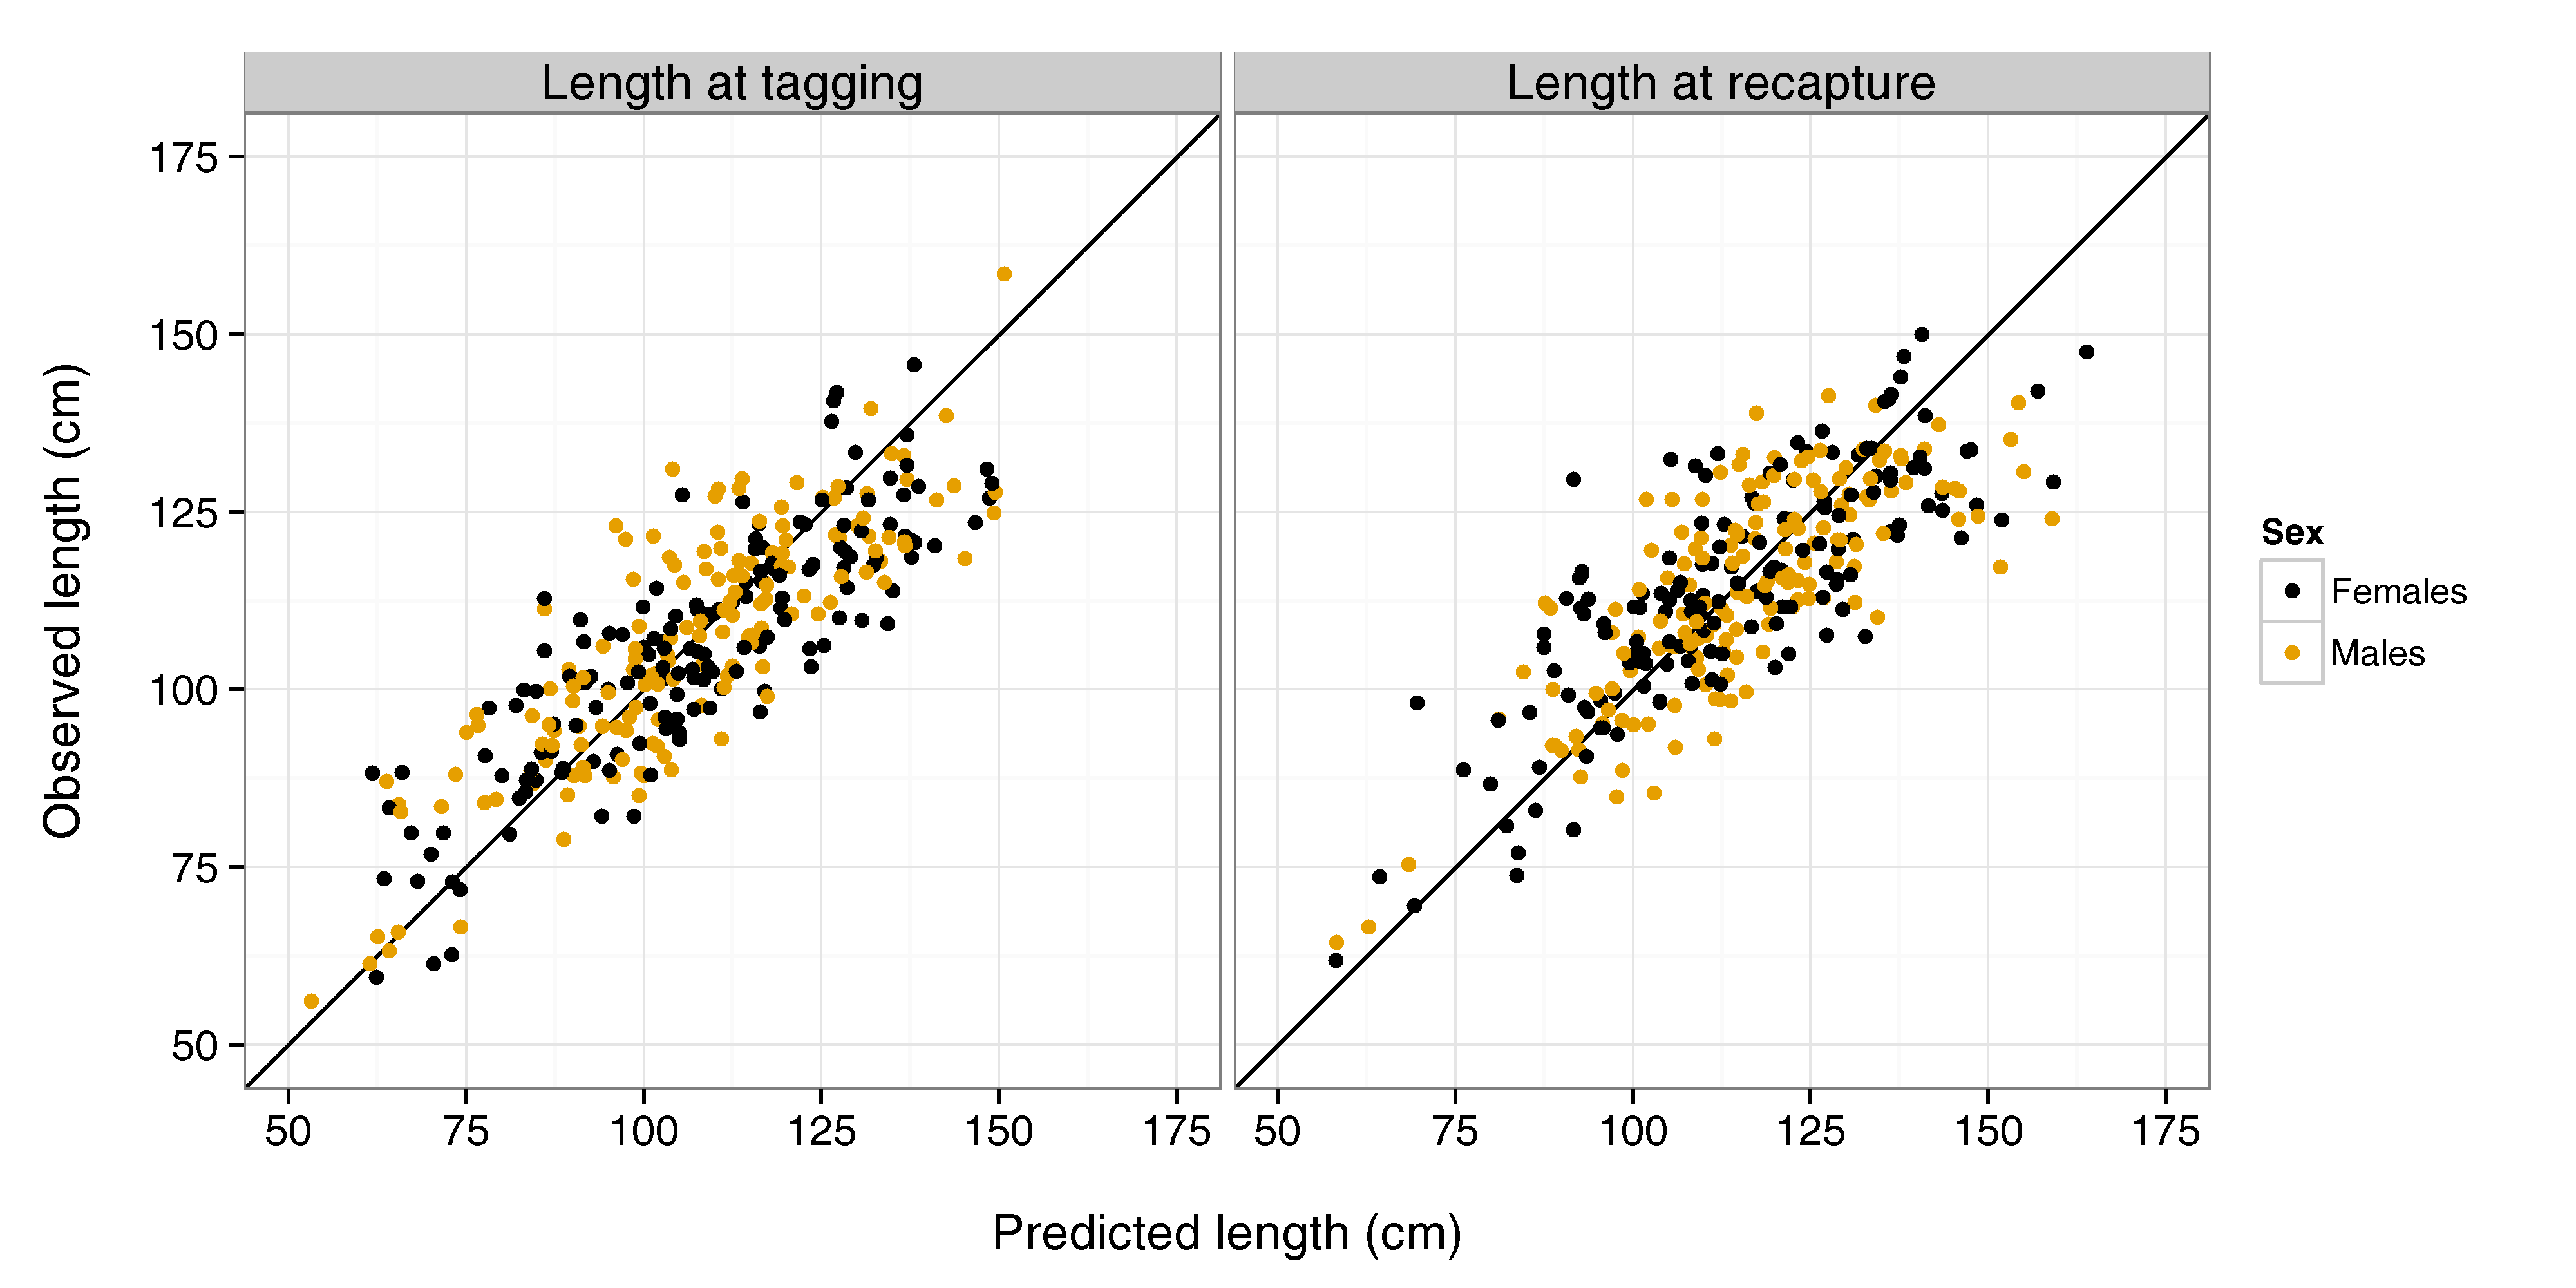
\includegraphics[width=\linewidth]{../simulation/sims2/results/ObsVsPred_3.png}
  \begin{quote}
    \caption{The first pdH simulation (sim 3).}
    \label{fig:sims2-fits}
  \end{quote}
\end{figure}
